%!TEX encoding = UTF-8 Unicode
\documentclass[master,korean,final]{cbnu-ecs}

% kaist.cls 에서는 기본으로 dhucs, ifpdf, graphicx 패키지가 로드됩니다.
% 추가로 필요한 패키지가 있다면 주석을 풀고 적어넣으십시오,
%\usepackage{...}
%

%\usepackage{kotex}
\usepackage{multirow}
\usepackage{varwidth}
\usepackage{amsmath}
\usepackage{indentfirst}
\usepackage{algorithm,algpseudocode}
\usepackage{booktabs}
\usepackage{longtable}

%\usepackage{xcolor}
%\renewcommand\tablename{표}
%\renewcommand\figurename{그림}

\newtheorem{theorem}{Theorem}	


% @command title 논문 제목
% @options [default: (none)]
% - korean: 한글제목 | english: 영문제목
\title[korean]{사각형 특징의 자세 추정을 통한 Factor Graph 기반 비주얼 SLAM}
\title[english]{Factor Graph based Visual SLAM with Geometric Pose Estimation of a Rectangle Feature}

\author[korean] {이}{재 민}
\author[english]{Lee}{Jae-Min}

\advisor[major]{박 찬 식}{Chan sik Park}{signed}

\department{RO}

% @command studentid 학번
\studentid{2014298010}

% 논문제출일
\submitdate{2016}{6}{3}

% @command approvaldate 지도교수논문승인일
% @param   year,month,day 연,월,일 순으로 입력
\approvaldate{2016}{6}{3}

% @command refereedate 심사위원논문심사일
% @param   year,month,day 연,월,일 순으로 입력
\refereedate{2016}{6}{3}

% @command gradyear 졸업년도
\gradyear{2016}{8}

% 본문 시작
\begin{document}

% 목차 (Table of Contents) 생성
\tableofcontents
% 그림목차 (List of Figures) 생성
\listoffigures
% 표목차 (List of Tables) 생성
\listoftables
% 영문초록 (abstract)
\begin{abstract}
%본 논문에서는 사각형 특징을 이용하여 위치와 자세를 복원하고 그를 factor graph형태로 구성하여 위치 인식과 특징 지도를 작성하는 방법을 제안하였다. 임의의 영상 평면 상 사변형이 입력으로 주어졌을 때 선분카메라쌍 알고리즘을 이용하여 종횡비를 알 수 없는 실세계의 직사각형을 해석적으로 복원하고, 그를 이용하여 homography를 구성하여 미리 알려진 카메라의 내부 파라미터 성분을 이용하여 정규화 한 뒤 카메라와 사각형 특징간의 상대 위치와 자세를 복원하였다. 이 때 사각형의 실제 크기를 알 수 없어 생기는 모호성을 해결하기 위해 카메라의 스테레오 구성을 가정한다. 스테레오 카메라가 x축에 대해 정렬되어있고 baseline값이 고정되어 있을 때 사각형과 카메라 사이의 정확한 위치와 자세를 추정하는 방법에 대해 제안하고 실험을 통해 특징 추출이 잘 이루어졌을 때 제안하는 위치 및 자세 추정의 성능이 준수함을 보였다. 추출된 특징과 상대 위치는 factor graph형태로 구성하고 negative log likelyhood 추정으로 접근하여 비선형 최소자승 문제를 정의한 뒤, 선형화를 통해 선형 최소자승 문제로 치환하여 cholesky factorization을 통해 해를 구한다. 이 때 사용할 수 있는 사각형 특징 추출 방법으로 선분 추출 기반의 방법과 영상 분할 기반의 방법을 제안하고 영상 분할 기반의 접근이 보다 유효함을 주장하였다. 제안한 전체 시스템은 카메라 기반의 위치 추정 시스템의 성능 분석용으로 널리 사용되는 KITTI Benchmark Suite위에서 실험이 수행되었다.\\
In this paper, a visual simultaneous localization and mapping(SLAM) method which uses rectangle features is proposed in factor graph manner.
Using the rectangle reconstruction method called coupled line camera algorithm which calculates analytically the aspect ratio of the rectangle from perspectively warped quadrilateral in the image plane, the plane homography is derived. The stereo configuration of the camera is proposed in order to solve the ambiguity arising from we not know the true size of the rectangle without additional information with corresponding modification of the coupled line camera algorithm to reconstruct the rectangle even the scale. A relative pose between rectangle in the real world plane and the camera is calculated for each quadrilateral from normalized homography with the intrinsic parameters of the camera which is constant in images captured by the identically same camera. the performance of this pose estimation method is showed in the simulated environment with ground truth value. 
Extracted feature and the relative position are consisted factor graph form and formulated in a nonlinear least-squares problem of the negative log likelyhood estimation of the graph. this problem is derived to the linear least squares problem through the linearization and solved by cholesky factorization for efficient calculation. And rectangle feature extraction methods are proposed by the line extraction based method and image segmentation based methods that is more effective approach than line extraction based method. the experiment was performed for the entire rectangle feature based SLAM system on KITTI Benchmark Suite that is widely used for analysis of the performance of the camera-based pose estimation system.

\end{abstract}

% 위의 세 종류의 목차는 한꺼번에 다음 명령으로 생성할 수도 있습니다.
%\makecontents

\pagenumbering{arabic}

\chapter{서론}
\section{연구 배경}

%{일반적인 SLAM연구}
자율 이동 로봇의 성공적인 임무 수행을 위해서는 주변 환경의 정보를 정합하고 자신의 위치를 파악하여 목표로의 접근을 위한 구동을 결정할 수 있어야 한다. 이 때 화성 탐사선, 재난 구조 로봇, 탄광 탐사로봇과 같이 사전에 정보가 주어지지 않은 환경에 놓인 로봇은 취득한 환경정보를 이용하여 스스로 지도를 작성하고 그 위의 자신의 위치를 추정하며 임무를 수행하여야 한다. 이러한 기술을 SLAM(Simultaneous Localization and Mapping)이라 하고 1986년 IEEE Robotics and Automation Conference에서 확률론적으로 문제에 접근하는 방안에 대한 토의를 가진 이후 이를 기반으로 연구가 계속되고 있다\cite{Durrant2006}. 확률론으로 SLAM문제를 수식화하여 계산하기 위해 전통적으로 Extended Kalman Filter\cite{Dissanayake2000}, Unscented Kalman Filter\cite{Martinez2005}, Extended Information Filter\cite{Thrun2003}, Rao-Blackwellized Particle Filter\cite{Montemerlo2002}등의 recursive bayesian filtering기술이 응용되었다. 이후 SLAM문제를 Belief Network, Markov Random Field등의 그래프 모델로 표현하고 그래프 최적화 기술을 이용하여 해결하고자 하는 시도가 이어졌고\cite{Kummerle2011}, 
현재까지 많은 연구자들이 이 접근법을 바탕으로 SLAM기술의 계산 복잡도, loop closure, 동적으로 변하는 환경 등에 대한 문제를 강인한 특징 추출 방식 제안 및 센서 처리 방식 개선, 지도 표현 방식 변경과 같은 다양한 방법으로 해결하고자 하는 노력이 이어지고 있다.\\
알려지지 않은 환경의 정보를 취득하기 위해 어떤 센서를 사용할 것인지 결정하는 것은 SLAM기술의 구제척인 형태와 성능을 크게 좌우한다. 센서로는 거리정보 기반의 LiDAR(Light Detection and Ranging)센서와 Sonar(Sound Navigation and Ranging)센서, RF(Radio Frequency) 또는 자기장을 이용한 인공 표식 인식 센서 그리고 카메라 등이 이용될 수 있다. 그러나 자율 이동 로봇이 임무를 수행하기 위한 환경 중 우주나 재해환경, 접근 불가 지역과 같이 사람의 접근과 활동의 제약이 존재하는 환경에서 인공 표식을 사전에 설치하여 SLAM에 활용하는 것은 굉장히 제한적일 수 밖에 없다. 따라서 SLAM에 관련된 많은 연구와 적용 사례들은 주어진 환경을 직접 추출할 수 있는 거리-방향 센서를 사용하여 문제를 정의하며 해결하고 있다. 그 중 자율 이동 로봇의 응용으로 가장 많이 연구되고 있는 두 센서는 LiDAR와 카메라로, 단일 센서를 이용한 연구는 물론 복수의 센서 또는 융합 센서 시스템을 구성하여 SLAM문제를 해결하는 연구도 활발하게 진행되어 왔다.\\
LiDAR는 센서로 부터 송출된 적외선의 Time-of-Flight를 응용하여 2차원 혹은 3차원 환경에 대한 거리 정보를 취득하는 능동형 센서이다. 충분히 강한 출력의 광원이 사용된다면 조명에 강인하고 일정한 검출 시간과 성능을 보장받을 수 있는 장점이 있으나 고정밀기계장치를 이용하여 충격에 민감하고 가격이 고가이다. 또한 점군으로 표현된 환경에 대한 거리정보는 취득 영역의 부피에 비해 비교적 적은 수 이고, 신호 세기 등 거리 이외의 정보는 취급이 어렵거나 사용이 제한적이기 때문에 데이터의 정보량은 비교적 적다고 할 수 있다. 카메라는 외부의 광원에서 발해져 직접 투사되거나 주변 물체에 반사되어 들어온 가시광선 근방의 전자기파에 대한 정보를 취득하는 감응형 센서이다. 주변 광원의 상태에 따라 사용에 제약을 받을 수 있으나 저렴한 가격에 고밀도의 환경정보를 취득할 수 있는 장점이 있다. 연산에 사용되는 로봇의 컴퓨터 혹은 연구용 워크스테이션의 성능이 높아지면서 보다 방대한 자료를 빠르게 처리할 수 있게 되어, 최근에는 저가에 풍부한 환경 정보를 취득할 수 있는 카메라를 이용하는 SLAM기술의 연구가 각광을 받고 있다. 또한 두 센서의 장점을 살려 융합 시스템을 구축, 활용하는 방법도 제시되어 있다\cite{Newman2006}.\\
%{카메라를 이용하는 SLAM 연구}
단안카메라를 이용하여 SLAM문제를 해결하고자 하는 초기 시도는 Lowe의 SIFT(Scale Invariant Feature Transform)를 이용한 SLAM\cite{Se2005}과 particle filter를 이용한 SLAM\cite{Eade2006}, extended kalman filter를 기반으로 단안 카메라를 이용한 실시간 SLAM방법\cite{Davison2007}이 있다. 이 후 이동 로봇 분야에서의 위치 추정 및 지도 작성 문제에 대해 카메라를 이용한 접근의 유효성이 입증 된 이후 후속 연구가 활발하게 연구가 진행되고 있다. 컴퓨터 비전 분야에서는 카메라를 이용하여 주어진 환경의 3차원 정보를 재구성하는 Structure from motion(SfM)이라는 문제가 로봇에서 통용되는 SLAM과 유사하다. 전통적인 SfM은 사전에 취득한 데이터에 대해 Bundle Adjustment\cite{Triggs2000}기법을 사용하여 연산 시간에 무관하계 고정밀의 결과를 얻는 것에 초점을 맞추고 있다. 근래들어 증강현실 등 실시간 처리 방법의 필요성이 대두됨에 따라 병렬연산과 Local Bundle Adjustment기법을 이용하여 실시간 SfM문제를 해결하는 방법\cite{Klein2007}이 제안되면서 카메라를 이용한 위치 인식 및 지도 작성에 대한 연구의 다른 접근 방식이 정립되었다. 이에 따라 로봇 분야에서 전통적으로 사용되던 Recursive filtering방식과 컴퓨터 비전 분야에서 사용되던 graph optimization방식에 대한 분석\cite{Strasdat2010}이 이루어졌고 연산 속도, 정확도, scalability등을 종합적으로 고려하였을 때 후자의 접근이 보다 바람직함을 제시하였다. 최신의 연구에서는 향상된 컴퓨터 성능과 General Purpose Graphic Processing Unit(GPGPU)의 사용이 용이해지면서 영상에서 특징을 명시적으로 추출하지 않고, 영상의 세기 정보를 직접 이용하여 카메라를 이용하여 실시간으로 SLAM을 해결하는 방법들이 제안되었다\cite{Forster2014b,Engel2014}.\\
%{Loop closure}
SLAM에서는 정적인 환경에서의 위치 추정 및 지도 작성의 정확도 뿐 아니라 센서의 오작동이나 kidnapping등의 요인으로 불연속적인 위치 변화가 발생하거나 동적으로 변화하는 환경에 강인한 시스템을 구성하는 것도 중요한 문제로 여겨져 왔다. 일부에서는 생물해부학적 지식을 활용하여 설치류의 공간 지각 시스템을 모방하여 통계학적 추정을 기반으로 하는 기존의 것과 완전히 구별되는 시스템을 제안하여 동적인 환경 변화에 대해 대처하고자 하는 시도가 있었다\cite{Milford2008}. 근래의 연구에서는 환경 변화에 대처하기 위해 기존의 SLAM시스템에 장소 인식 방법을 이용하여 성능을 보완하는 형태로 연구가 진행되어 왔다. 특징의 복잡도가 높지 않은 저 수준의 시각 특징으로 Chow-liu tree구조의 Bag-of-words를 구성하여 장소 인식을 수행하는 방법\cite{Cummins2011}이 정확도와 속도에서 우수한 성능을 보이고 있어 많은 후속 연구들이 이에 기반을 두고 있다. Loop closure 검출을 위해 장면이라는 고수준의 특징을 사용하여 반경 1000km수준의 대규모 환경, 운행 기간 1년 이상의 장기 구동, 눈, 비 등의 기후 변화에도 강인하게 SLAM 문제에 대처할 수 있는 연구도 진행되었다\cite{Milford2012}.\\
%{SLAM에서 고차원 특징 추출 시도 사례}
점 특징 기반의 SLAM이 가지는 한계를 타파하기 위해 다른 형태의 시각 특징을 이용하는 접근도 연구되고 있다. Li의 연구에서는 연속된 영상에서 추출한 광류(optical flow)를 이용해 평면 특징을 이용하여 위치 추정 오차를 줄이고자 시도하였고\cite{Li2014}, Lu의 연구에서는 기존의 점 특징과 함께 선분, 직선, 평면, 소실점 등을 그래프로 구성하여 추가된 기하 정보를 이용하여 정밀한 위치 추정을 가능케 하였다\cite{Lu2015}. RGB-D카메라를 통해 얻을 수 있는 추가적인 공간 정보를 함께 표현한 점구름 형태의 3차원의 물체 구분하고 3차원 강체 움직임을 가지는 표식으로서 SLAM에 사용한 연구도 있다\cite{Moreno2013}.
\section{연구 목적 및 제안}
이와 같이 카메라를 이용한 SLAM의 성능을 향상시키기 위한 다양한 시도가 있었다. 정리하면 점 특징을 추출하여 여러 장의 영상에서 특징간 정합을 통해 로봇 또는 카메라의 위치와 자세를 추출하여 SLAM문제를 풀어왔고, 국소 패치를 기반으로 하는 특징 기술자를 개선하여 연속된 영상간 정합이 아닌 임의의 위치와 자세 간의 상관 관계를 계산하여 보다 정밀한 지도를 계산하는 loop closure 성능을 개선하였다. 보다 정밀한 위치 추정을 위해 선분, 평면 등의 다양한 기하 특징을 추가로 도입하여 향상된 정확도를 얻었다.
그러나 제안된 연구들에서는 정밀한 위치 추정을 위한 시각 특징 개선과 loop closure성능 향상을 위한 특징 기술자의 성능 개선을 별도의 문제로 접근한다. 전자의 접근에서는 특징의 기술자 자체는 점 특징 기반의 기존 SLAM과 크게 다르지 않고, 후자는 국소 패치를 기반으로 별도의 장면 인식 시스템을 구축하여 기존 시스템과 융합하는 방식으로, 국소 패치를 대체할 수 있는 수준의 특징 자체에 대한 개선을 염두에 두지 않고있다. 
야지 환경을 제외하고는 방, 복도 등의 실내 환경과 건물이 존재하는 도심지와 같은 실외 환경에서는 Figure \ref{envexample}과 같은 타일, 창문, 게시판, 간판, 표지판 등의 다양한 직사각 형태를 가진 물체를 볼 수 있다. 이러한 직사각형 물체는 내부의 재질, 색상이 서로 구분 가능한 경우가 많고 특징이 가지는 정보량이 점 형태에 비해 많으며, 시각 정보를 의미론적으로 분할하기 위해 사용할 수 있는 가장 쉽게 찾을 수 있는 기하학적 형태이다. 본 논문에서는 점 기반의 시각 특징을 대체하기 위한 사각형을 이용한 고수준 시각 특징 기반 visual SLAM 방법을 제안한다.
\begin{figure}[!ht]
  \centering
	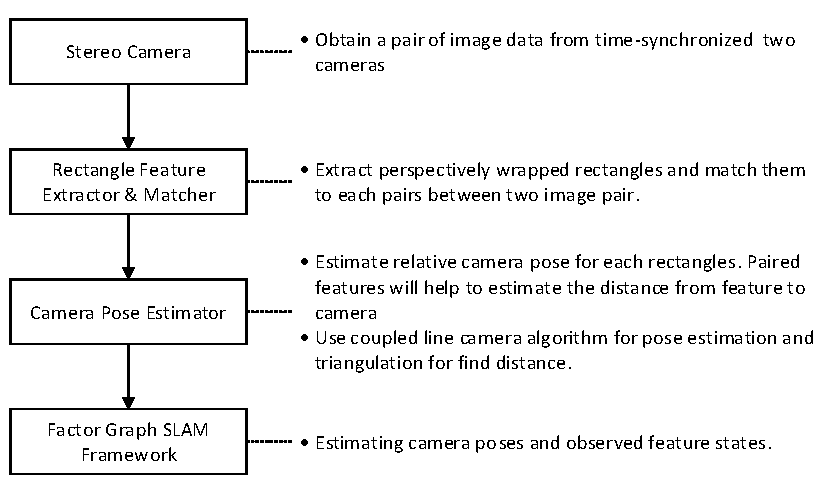
\includegraphics[width=400px]{img/Rectangle_feature_SLAM_framework_cropped.pdf}
  \caption{The proposed rectangle feature SLAM framework}
\label{rectSLAM_framework}
\end{figure}

논문의 구성은 첫 째로 하나의 영상에서 주어진 임의의 사변형을 투영변환의 불변성질을 이용하여 원본 직사각형으로 복원하는 선분카메라쌍 알고리즘을 통해 카메라와 특징간의 상대 위치와 자세를 추정하는 방법에 대해 설명한다. 단일카메라에서 얻은 영상에서 선분카메라쌍 알고리즘을 이용하여 복원한 직사각형은 실제 크기를 알 수 없어, 그 크기를 임의의 값으로 가정하고 결과를 도출한다. 따라서 하나의 장면에서 다수의 사각형 특징을 이용하여 위치 추정을 할 경우 특징 간의 스케일 정보를 알 수 없어 올바르게 공간 상의 위치 추정을 할 수 없다. 스테레오 카메라의 기하 관계를 이용하여 특징의 크기 모호성 문제를 해결하는 방법을 제시한다. 이와 같이 추출된 사각형 특징울 카메라의 위치 및 자세와 함께 factor graph로 표현하여 전체 경로 및 특징 지도를 추정하는 방법을 제안한다. 또한 추출된 사각형 특징 간의 유사도를 파악하기 위한 특징 기술자를 제안한다. 
\newpage
\begin{figure}[!ht]
  \centering
	\includegraphics[width=360px]{img/BroadwayPlayers_01_merged.png}
  \caption{An example of rectangle object segmentation in urban environment : Sign plates(blue), windows(red), wall(green), pillar(yellow)}
\label{envexample}
\end{figure}

\newpage
%%%%%%%%%%%%%%%%%%%%%%%%%%%%%%%%%%%%%%%%%%%%%%%%%%%%%%%%%%%%%%%%%%%%%%%%%%%%%%%%%%%%%%%%%%%%%%%%%%%%%%%%%%%%%%%%%%%
%%%%%%%%%%%%%%%%%%%%%%%%%%%%%%%%%%%%%%%%%%%%%%%%%%%%%%%%%%%%%%%%%%%%%%%%%%%%%%%%%%%%%%%%%%%%%%%%%%%%%%%%%%%%%%%%%%%
%%%%%%%%%%%%%%%%%%%%%%%%%%%%%%%%%%%%%%%%%%%%%%%%%%%%%%%%%%%%%%%%%%%%%%%%%%%%%%%%%%%%%%%%%%%%%%%%%%%%%%%%%%%%%%%%%%%
\chapter{사각형 특징의 기하학적 성질을 이용한 스테레오 카메라의 자세 복원 방법}

%\section{렌즈왜곡 모델}
%\section{자세 추정을 위한 사각형 복원 방법}
\section{평면 Homography를 이용한 카메라의 자세 복원 방법}

종래의 방법으로는 복수의 영상 간 점 특징을 정합하여 자세를 추정한다. 2장의 이미지에 대한 카메라 기하 관계는 epipolar constraint로 표현되며 이를 이용하여 fundamental matrix 또는 essential matrix를 추정하고 두 영상에 대한 카메라 자세 변화를 얻는다. 3개의 이미지에 대해서는 trifocal tensor를 이용하여 카메라 기하관계가 표현된다. 각각의 방법에 대해서는 Nister의 5-point RANSAC 알고리즘\cite{Nister2005}과 Guerrero의 연구\cite{Guerrero2008}가 그 예시이다. 이미지와 카메라간의 n-view geometry에 대해서는 hartley의 저서\cite{Hartley2003}에 보다 상세하게 설명되어 있다.\\
본 논문에서 집중 할 것은 1장의 이미지에 대한 카메라 기하 관계인 homography를 이용하여 카메라의 자세를 추정하는 것이다. Homography는 두 평면 사이의 변환을 표현하는 행렬로, 직사각 특징의 네 점이 한 평면 위에 있다는 가정을 두고 카메라의 자세를 복원한다. 이 접근에서는 2장 이상의 연속된 영상에서 5쌍 이상의 정합된 점을 필요로 하는 기존 방법에 비해 1장의 이미지에서 4개의 점 만으로 유일하게 카메라와 특징간의 상대 자세를 추정할 수 있다는 장점이 있다. \\
일반적인 카메라의 투영을 선형 사상으로 표현한다면 동차좌표계를 이용하여 식 \eqref{homography}과 같이 나타낼 수 있다.

\begin{equation}
\begin{bmatrix} x1'\\x2'\\x3' \end{bmatrix} = \begin{bmatrix} p_{11} & p_{12} & p_{13} & p_{14} \\ p_{21} & p_{22} & p_{23} & p_{24}\\ p_{31} & p_{32} & p_{33} & p_{34} \end{bmatrix}\begin{bmatrix} x1\\x2\\x3\\x4 \end{bmatrix} \label{homography}
\end{equation}

참고로 위의 투영 변환을 모델하기 위해 식 \eqref{pinhole}의 pinhole 카메라 모델을 사용하기도 한다. 이 모델은 렌즈 왜곡에 대한 영향을 무시하고 초점거리, 광축 중심 등의 값으로 이루어진 내부 파라미터 행렬과 카메라의 상대 위치와 자세 정보로 이루어진 외부 파라미터 행렬로 이루어져 있다.

\begin{equation}
s\begin{bmatrix} u\\v\\1 \end{bmatrix} = \begin{bmatrix} f_{x} & s_{skew} & c_{x} \\ 0 & f_{y} & c_{y} \\ 0 & 0 & 1 \end{bmatrix}\begin{bmatrix} r_{11} & r_{12} & r_{13} & t_{X} \\ r_{21} & r_{22} & r_{23} & t_{Y}\\ r_{31} & r_{32} & r_{33} & t_{Z} \end{bmatrix}\begin{bmatrix} X\\Y\\Z\\1 \end{bmatrix} \label{pinhole}
\end{equation}
이는 간단하게 $\mathrm{x}'=K[R|t]\mathrm{x}$로 표현 할 수 있다.
\begin{figure}[!ht]
  \centering
	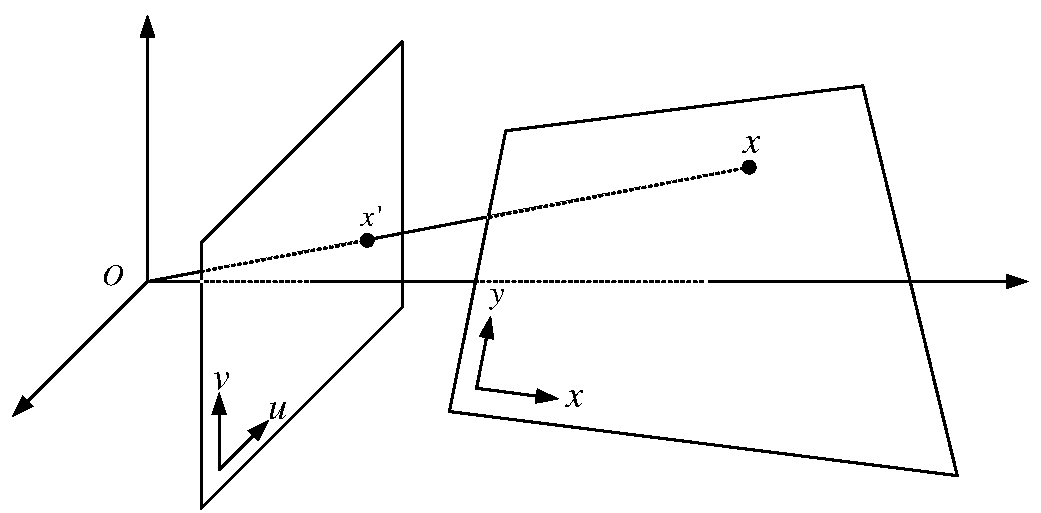
\includegraphics[width=240px]{img/planar_homography_cropped.pdf}
  \caption{The configuration of planar homography with respect to corresponding points }
\label{planar_homography}
\end{figure}
이 때 투영되는 대상이 어떤 평면 위의 점이라면 $Z=0$임을 이용하여 동차좌표계를 위에서 평면 homography 관계를 식\eqref{planar_homography}와 같이 선형방정식으로 표현할 수 있다.

\begin{equation}
\begin{bmatrix} x1'\\x2'\\x3' \end{bmatrix} = \begin{bmatrix} h_{11} & h_{12} & h_{13} \\ h_{21} & h_{22} & h_{23} \\ h_{31} & h_{32} & h_{33} \end{bmatrix}\begin{bmatrix} x1\\x2\\x4 \end{bmatrix} \label{planar_homography}
\end{equation}

이는 간단하게 $\mathrm{x}'=H\mathrm{x}$로 표현 할 수 있고, 이 때 $R=[r_1 \ r_2 \ r_3]$ 이라 하면 $H=K[r_{1} \  r_{2}|t]$이다.
$R$은 정규직교행렬이므로 식 \eqref{rotation_matrix}와 같이 복원할 수 있다.
\begin{equation}
R=\begin{bmatrix}r_1 && r_2 && r_1\times r_2\end{bmatrix} 
\label{rotation_matrix}
\end{equation}

여기서 동차좌표계를 이용한 이와 같은 표현에서 스케일에 대한 정보는 알 수 없으므로 $rank(H)=8$이다. 따라서 두 평면 위의 서로 대응되는 점 쌍으로 평면 homography를 완전하게 추정하기 위해서는 적어도 4개의 쌍이 필요하다. 일반적으로는 카메라의 촬상면에 대응되는 점 만이 직접 측정이 가능하고 실세계의 대응점은 구하기 어려우므로 chessboard를 이용한 카메라 캘리브레이션을 수행할 때와 같이 이미 4개의 점에 대한 형태 정보를 알고 있는 특수한 경우가 아니면 정상적인 자세를 추정할 수 없다.

\section{선분 카메라쌍 방법을 이용한 사각형 복원 방법}
본 논문에서는 영상 위의 4개의 점에 대응되는 실세계의 대응 점가질 수 있는 형태 중 직사각형일 경우 가지게 되는 기하적 성질을 이용하여 완전하게 카메라의 자세를 추정하는 방법에 대해 설명한다. 먼저 영상 위의 4개 점을 선분카메라쌍 알고리즘\cite{Lee2012,Lee2013}을 이용하여 원본 사각형의 종횡비를 복원한다. 이 알고리즘은 투영 변환의 불변성인 colinearity를 바탕으로 영상 위의 선분과 실제 선분간의 관계를 Figure \ref{linecamera}와 같은 가상의 선분 카메라 모델로 표현한다. 그러나 하나의 선분카메라만으로는 유일하게 투영 중심을 복원해낼 수 없다. 이에 직사각형을 구성하는 대각선 두 쌍에 대해 선분카메라 모델을 적용할 경우, Figure \ref{coupled_linecamera}와 같이 두 선분카메라의 실제 평면 상 직선의 교차점이 두 직선을 등분하는 점이며 두 선분카메라의 투영중심은 동일하다는 조건을 추가로 이용할 수 있다. 이 조건에 의해 투영변환의 불변성 중 하나인 cross ratio를 이용하여 유일하게 사각형의 종횡비와 그에 대응하는 투영 중심을 복원할 수 있다. Table \ref{CLC_algorithm}에 선분카메라쌍 알고리즘이 기술되어 있다. 복원한 종횡비를 토대로 영상 평면 위 사변형의 꼭지점에 대응되는 실세계 상에서 직사각형의 꼭지점의 좌표를 구성하고 평면 homography를 구해 이전 장의 방법을 이용하여 카메라의 위치와 자세를 추정한다. 이 때 추정되는 위치는 식 \ref{pc_clc}와 같다.
\begin{equation}
\label{pc_clc}
p_c = \frac{d}{\sin\phi}(\cos\theta_0\sin\phi,\ -\cos\theta_0\cos\phi+\cos\theta_1,\ \sin\theta_0\sin\theta_1\sin\rho)
\end{equation}
\\
그러나 선분카메라쌍 기반의 사각형 복원 방법은 원본 사각형의 중점이 정확히 영상의 중심점과 대응되는 특별한 경우에 한하여 적용이 가능하다. 이를 보완하기 위해 소실선의 성질을 이용하여 주어진 사각형에 대해 합동이면서 영상에 대응되는 중심점이 광축에 정렬되는 가상의 사각형을 추출하는 방법이 있다\cite{Lee2014}. 먼저 Figure \ref{offcentered}의 직선 $\overleftrightarrow{w_0 w_1}$을 작도한다. 실세계의 직사각형에 대응되는 두 사변형의 대변을 연장하여 교차점을 찾거나, 별도의 소실점 추정 알고리즘을 사용하여 정렬하고자 하는 사변형에 대응되는 두 개의 소실점을 구한 뒤 직선으로 잇는다. 이렇게 작도한 소실선에서 원본 사변형의 중점과 각 꼭지점을 지나는 직선들과 만나는 두 점을 $w_{d,0}$, $w_{d,1}$이라 할 때, 이 두 점과 영상 중심 $o_m$을 지나는 직선을 작도한다. 원본 사변형의 중심과 영상 중심을 지나는 직선 $\overleftrightarrow{o_m u_m}$이 소실선 $\overleftrightarrow{w_0 w_1}$와 교차하는 점을 $w_m$이라 할 때, 이 점과 원본 사변형의 각 꼭지점을 지나는 직선과 $\overleftrightarrow{w_{d,0} o_m}$, $\overleftrightarrow{w_{d,1} o_m}$ 두 직선들과 이루는 교점을 구하여 중심에 정렬된 사변형을 얻을 수 있다. 이 사변형은 역투영변환 시 원본 사변형에 대응되는 직사각형과 합동인 직사각형을 만들어 내는 성질이 있다. 이는 소실선 위의 점 $w_m$와 사변형의 각 꼭지점을 이은 선분은 원본 직사각형의 스케일변화가 그리는 사각기둥을 두 소실점으로 표현된 투영변환에 의해 영상에 투영된 형태임에 기인한다.
\begin{table}[!t] 
\caption{The coupled line camera algorithm for the rectangle reconstruction}
\label{CLC_algorithm}
\begin{tabular}{p{360pt}}
\toprule[1.5pt]
\textbf{Algorithm} The coupled line camera algorithm for the rectangle reconstruction\\
\hline

\textbf{Input}		$l_i$ - a lenght of line camera, $i=0,1,2,3$.
					$\rho$ - a cross angle of the quadrilateral diagonal.\\
\textbf{Output}		$\phi$ - the crossing angle of rectangle
\\

\hline
\begin{algorithmic}[1]
\For{$i=0,1$}
\State Find division ratio coefficient
\[
\alpha_i = \frac{l_i - l_{i+2}}{l_i + l_{i+2}}.
\]
\EndFor
\State Find relative lenght coefficient
\[
\beta = \frac{l_1}{l_0}.
\]
\State Find lenght of principle axis
\[
d = \sqrt{\frac{(1-\alpha_1)^2\beta^2-(1-\alpha_0)^2}{\alpha_0^2(1-\alpha_1)^2\beta^2-\alpha_1^2(1-\alpha_0)^2}}.
\]
\For{$i=0,1$}
\State Find $\theta_i$ w.r.t
\[
cos\theta_i = d\alpha_i
\]
\EndFor
\State Find $\phi$ w.r.t
\[
	\cos{\phi} = \cos{\theta_0}\cos{\theta_1} + \sin{\theta_0}\sin{\theta_1}\cos{\rho}
\]
\end{algorithmic}\\
\toprule[1.5pt]
\end{tabular}
\end{table}

\newpage

\begin{figure}[!ht]
  \centering
	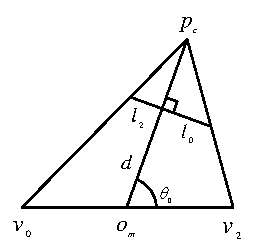
\includegraphics[width=220px]{img/linecamera_cropped.pdf}
  \caption{The configuration of single line camera model}
\label{linecamera}
\end{figure}
\begin{figure}[!ht]
  \centering
	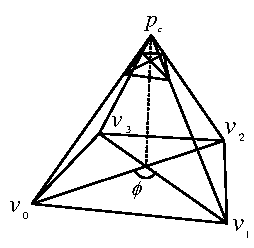
\includegraphics[width=220px]{img/coupled_linecamera_cropped.pdf}
  \caption{The configuration of coupled line camera model with a rectangle}
\label{coupled_linecamera}
\end{figure}
\newpage
\begin{figure}[!ht]
  \centering
	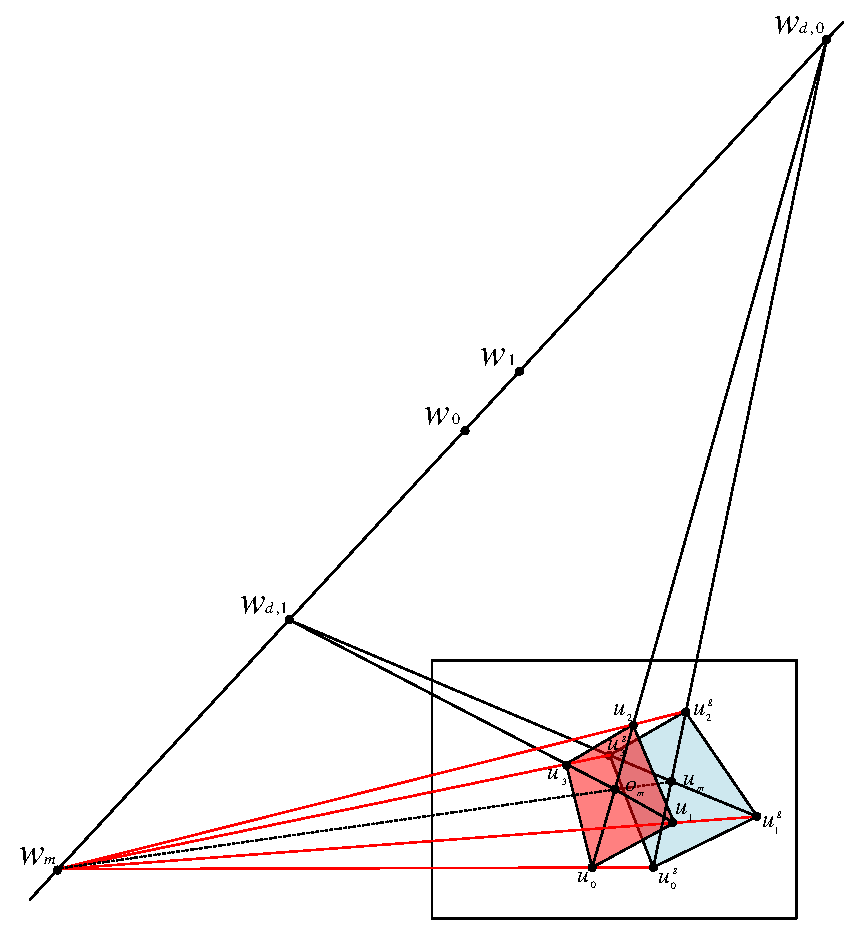
\includegraphics[width=360px]{img/offcentered_cropped.pdf}
  \caption{Off-Centered quadrilateral alignment with maintaining congruency}
\label{offcentered}
\end{figure}


\newpage

\section{3차원 자세 추정을 위한 스테레오 카메라 기반의 선분카메라쌍 방법}
단안 카메라에서 취득한 영상만으로는 3차원 공간 상 특징의 위치를 결정할 수 없다. 이는 투영변환에 의해 스케일에 대한 정보가 손실되기 때문이다. 상기한 선분카메라쌍 알고리즘 및 평면 homography를 이용한 사각형 기반 카메라 자세 추정 방법에서는 실제 크기 대신 중점과 각 꼭지점 간의 거리가 1인 사각형으로 가정한다. 이 경우 같은 장면에서 크기가 다른 복수의 사각형에 대한 위치 추정 결과는 모두 다른 스케일을 가지므로, 동일한 위치에서 촬영된 영상에서 추출한 위치임에도 불구하고 추정에 사용된 특징 별로 상이한 값을 보이게 된다. 이에 스테레오 카메라를 이용하여 특징의 3차원 공간 정보를 완전히 추정하고 한 영상 내부의 복수의 특징에서 추정한 카메라의 위치 및 자세 결과물을 효율적으로 사용하는 방법에 대해 서술한다. \\
스테레오 카메라는 두 pinhole 카메라가 $X$축으로만 $b$만큼의 변위를 가지는 Figure \ref{stereo_triangulation}와 같은 단순한 구조를 가지는 경우로 가정한다. 이 경우 두 카메라에서 3차원상의 점 $P$에 대응하는 점 쌍$X_1=(u_1,v_1)$,$X_2=(u_2,v_2)$에 대해 식 \eqref{stereo}의 관계를 $P$의 위치를 확정할 수 있음을 알 수 있다.
\begin{equation}
\label{stereo}
X=u_1*\frac{Z}{f}, \quad Y=v_1*\frac{Z}{f}, \quad Z=b*\frac{f}{u_1-u_2}
\end{equation}
식 \eqref{stereo}는 왼쪽 카메라를 기준으로 점 $P$의 위치를 표현한 것에 유의한다.\\
선분카메라쌍 알고리즘에서는 중심 정렬된 사각형에 대한 기하적 복원과 위치 추정을 수행한다. 위의 스테레오 카메라를 이용하여 얻을 수 있는 스케일 정보는 Figure \ref{depth_compensate}의 $||\overline{p_c u_m}||$이며 위치 추정 결과의 스케일 보상을 위해 필요한 정보는 직사각형의 중점과 카메라의 투영 중심 사이의 거리 $||\overline{p_c o_m}||$이다. 이는 $o_m$을 중점으로 하는 가상의 정렬된 직사각형을 원점으로 두고 삼각형 $\Delta p_c o_m u_m$에 사인법칙을 적용하여 유도할 수 있다.

Figure \ref{depth_compensate}에서 $||\overline{p_c o_m}||$을 $d$, $||\overline{p_c u_m}||$을 $d'$, 삼각형의 꼭지점인 $p_c$, $o_m$, $v_m$에 대한 각을 $\psi_1$, $\psi_2$, $\psi_3$이라 하고 평면 $\pi$에 대한 법선벡터를 $\overrightarrow{n} = [0 0 1]^T$이라고 둔다. 그 경우 $p_c$의 꼭지각 $\psi_1$는 Figure \ref{linecamera}와 같이 영상평면과 광축이 수직을 이루고, 그 교점을 $u_{om}$이라 할 때 직각삼각형의 성질을 이용하여 아래와 같이 구할 수 있다.

\begin{equation}
\label{angle_psi1}
\psi_1 = \tan^{-1}{\frac{||\overline{u_m u_{om}}||}{f}}
\end{equation}

$o_m$의 꼭지각 $\psi_2$은 평면 $\pi$의 법선벡터와 식 \eqref{pc_clc}를 이용해서 유도할 수 있다.

\begin{equation}
\label{angle_psi2}
\psi_2 = \frac{\pi}{2}-\cos^{-1}\frac{\overrightarrow{n}\cdot\overrightarrow{p_c}}{||\overrightarrow{n}||\ ||\overrightarrow{p_c}||}
\end{equation}

또한 삼각형 $\Delta p_c o_m u_m$에 대해 사인법칙에 의해 아래의 식이 성립한다.
\begin{equation}
\label{sine_rule}
\frac{d'}{\sin\psi_2} = \frac{d}{\sin\psi_3}
\end{equation}
이를 $d$에 대해 정리하면 식 \eqref{depth_compensate_result}와 같다.
\begin{equation}\label{depth_compensate_result}
\begin{split}
d & =\frac{d'}{\sin\psi_2}\sin\psi_3 \\
& =\frac{d'}{\sin\psi_2} \sin(\pi-(\psi_1+\psi_2)) \\
& =\frac{d'}{\sin\psi_2} \sin(\psi_1+\psi_2)
\end{split}
\end{equation}

이와 같이 얻은 $d$를 이용해서 정확한 위치를 얻기 위해 실제 사각형의 크기를 구하여야 한다. Figure \ref{linecamera}에서 직사각형의 중점에서 꼭지점까지 이은 선분에 해당하는 $||\overline{o_m v_0}||$의 거리를 $m$이라고 할 때 $d$와의 관계는 \eqref{rect_size}와 같다.
\begin{equation}
\label{rect_size}
m = d \frac{l_0}{f\sin\theta_0 + l_0\cos\theta_0}
\end{equation}
이를 이용해서 영상 위 원본 사변형의 꼭지점 $u_1$, $u_2$, $u_3$, $u_4$와 중심 정렬 된 직사각형의 꼭지점 $(m,0)$, $(m\cos\phi, m\sin\phi)$, $(-m, 0)$, $(-m\cos\phi, -m\sin\phi)$으로 평면 homography룰 구하여 카메라와 특징 간의 상대 자세를 복원할 수 있다.
\begin{figure}[!ht]
  \centering
	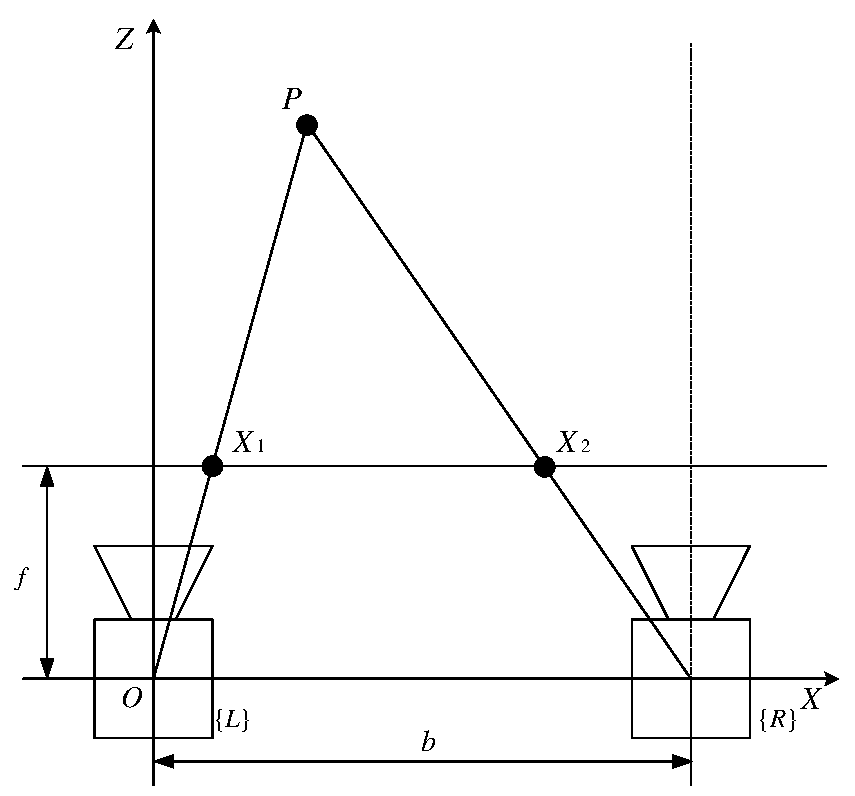
\includegraphics[width=360px]{img/stereo_triangulation_cropped.pdf}
  \caption{The configuration of simple stereo camera model}
\label{stereo_triangulation}
\end{figure}

\begin{figure}[!ht]
  \centering
	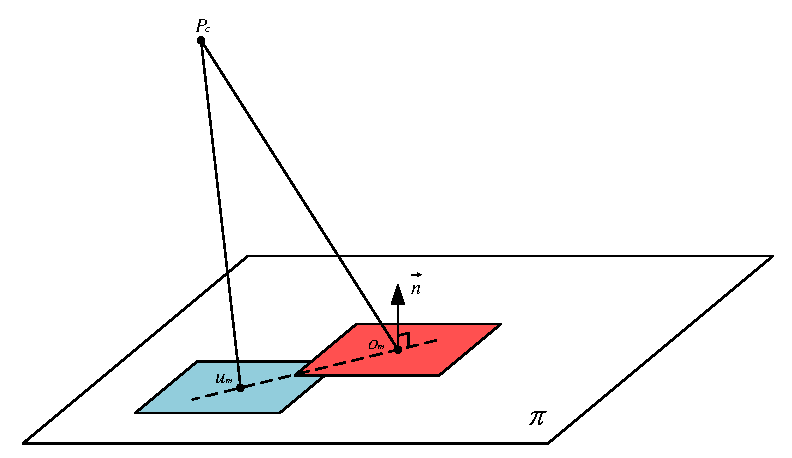
\includegraphics[width=360px]{img/depth_compensate_cropped.pdf}
  \caption{Distance compensation for off-centered rectangle}
\label{depth_compensate}
\end{figure}

%%%%%%%%%%%%%%%%%%%%%%%%%%%%%%%%%%%%%%%%%%%%%%%%%%%%%%%%%%%%%%%%%%%%%%%%%%%%%%%%%%%%%%%%%%%%%%%%%%%%%%%%%%%%%%%%%%%
%%%%%%%%%%%%%%%%%%%%%%%%%%%%%%%%%%%%%%%%%%%%%%%%%%%%%%%%%%%%%%%%%%%%%%%%%%%%%%%%%%%%%%%%%%%%%%%%%%%%%%%%%%%%%%%%%%%
%%%%%%%%%%%%%%%%%%%%%%%%%%%%%%%%%%%%%%%%%%%%%%%%%%%%%%%%%%%%%%%%%%%%%%%%%%%%%%%%%%%%%%%%%%%%%%%%%%%%%%%%%%%%%%%%%%%
\chapter{사각형 특징을 이용한 Factor Graph 기반 Visual SLAM}
\section{SLAM을 위한 Factor Graph 표현 유도}
복수의 사각형 특징 정보를 취합하여 특징지도 작성 및 위치 추정을 위하여 factor graph기반의 SLAM방법\cite{Dellaert2006}을 사용한다. Flitering 방법을 이용하는 접근과 다르게 이 방법에서는 로봇 또는 카메라의 현재 자세 만을 추정하는 것이 아니라 전체 경로를 추정한다. loop closure 문제를 별도로 다룰 필요 없이 구성한 factor graph를 최적화 하는 것으로 해결할 수 있어 보다 정확한 지도 작성이 가능하게 한다. 또한 희소 선형대수 기법을 응용하여 전통적인 kalman filter기반의 SLAM을 대체할 수 있는 속도 개선과 증분형 계산이 가능한 알고리즘을 제안하고 있어 목적에 따라 같은 시스템으로 batch 처리, 실시간 처리를 선택하며 성능을 유지할 수 있다\cite{Kaess2007, Kaess2011}.\\
종래에 SLAM문제의 그래프 표현은 belief network라는 형태가 많이 사용되었다. belief network는 어떤 확률 변수 집합에 대해 조건부 독립 구조를 시각적으로 나타낸 것이다. 그래프를 구성하는 각 노드들은 앞 노드에만 직접적으로 의존하는 형태로, 방향성이 있고 비 순환성인 구조로 표현된다. Figure \ref{belief_network}에 SLAM 문제를 belief network로 표현한 예시가 주어져 있다. Factor graph는 추정하고자 하는 확률밀도함수를 인수분해한 형태를 표현하는 무향성 양분 그래프(bipartite graph)의 일종이다. 이 형태는 marginal distribution의 효율적인 계산을 위해 주로 응용되는 형태이다. \\
$k$번째 로봇의 상태변수를 $x_k\in X \ (k\in{0,1,2,\dots,i})$, $m$번째 표식변수를 $l_m\in L \ (m\in{0,1,2,\dots,N})$, $n$번째 측정변수를 $z_n\in Z \ (n\in{0,1,2,\dots,j})$이라 하자. 
\newpage
\begin{figure}[!ht]
  \centering
	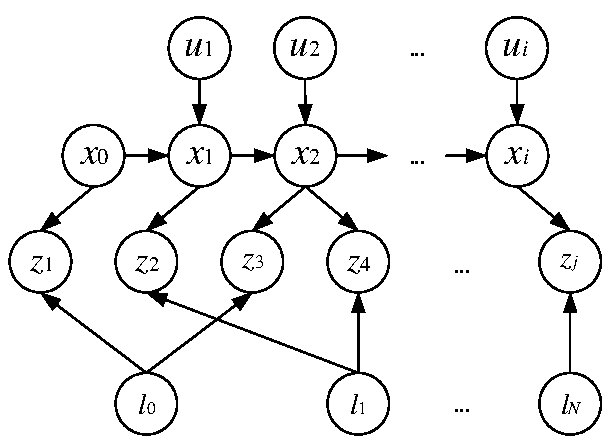
\includegraphics[width=300px]{img/beliefnetwork_cropped.pdf}
  \caption{The example of belief network model for SLAM framework}
\label{belief_network}
\end{figure}

\begin{figure}[!ht]
  \centering
	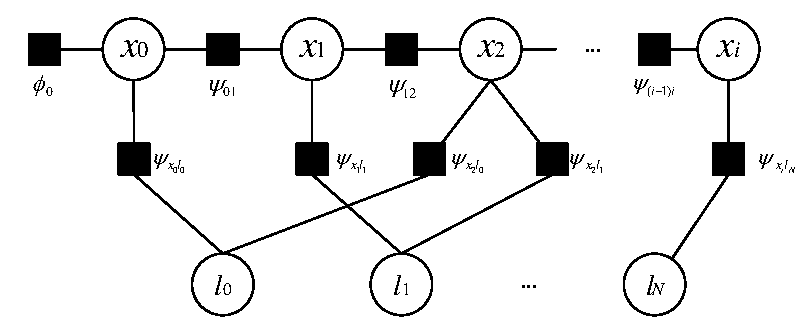
\includegraphics[width=410px]{img/factorgraph_cropped.pdf}
  \caption{The example of factor graph model for SLAM framework}
\label{factorgraph_diagram}
\end{figure}
\newpage

Belief network구조의 Figure \ref{belief_network}에 해당되는 결합확률은 식 \eqref{belief_joint_probaility}과 같이 표현할 수 있다.
\begin{equation}
\label{belief_joint_probaility}
P(X, L, Z)=P(x_0)\prod^i_{k=1}P(x_k|x_{k-1}, u_k)\prod^j_{n=1}P(z_n|x_{kn}, l_{mn})
\end{equation}
통상적으로 $P(x_k|x_{k-1}, u_k)$는 로봇의 모션 모델, $P(z_n|x_{kn}, l_{mn})$는 센서의 측정 모델이라 부른다.  여기서는 Data association문제를 고려하지 않고 $z_n$은 이미 알려져 있는 변수로 가정한다. 모델이 가우시안 분포를 따른다고 가정하면 로봇의 모션 모델을 식 \eqref{motion_model}과 같이 표현할 수 있다.
\begin{equation}
\label{motion_model}
x_k = f_i(x_{k-1}, u_k) + \omega_k,\ P(x_k|x_{k-1}, u_k)\propto \exp-\frac{1}{2}||f_k(x_{k-1}, u_k)-x_k||^2_{\Lambda_k}
\end{equation}
마찬가지로 센서 관측 모델 또한 가우시안으로 가정 할 경우 식 \eqref{measurement_model}와 같이 표현할 수 있다.
\begin{equation}
\label{measurement_model}
z_n = h_n(x_{kn}, l_{mn}) + \nu_k,\ P(z_n|x_{kn}, l_{mn})\propto \exp-\frac{1}{2}||h_n(x_{kn}, l_{mn})-z_n||^2_{\Sigma_n}
\end{equation}
이 때  $||x||^2_\Sigma=x^T\Sigma^{-1} x$는 공분산 $\Sigma$에 대한 마할라노비스 거리를 말한다. \\
Factor graph는 위의 belief network모델에서 자연스럽게 유도할 수 있다. 측정변수 $z$는 알려진 값이므로  표식과 로봇의 상태변수를 연결하는 결합확률 factor의 매개변수로 간주할 수 있다. 제어 입력 $u$또한 로봇 상태변수 간의 factor의 매개변수로 간주하면 Figure \ref{factorgraph_diagram}과 같이 나타낼 수 있다. 이렇게 구성된 factor graph는 알려지지 않은 로봇의 상태변수와 표식에 대응하는 노드와 $z$ 또는 $u$를 매개변수로 가지는 두 가지 종류의 factor를 가진다. 이를 일반적인 factor graph형태로 표현하면 모든 알려지지 않은 변수$\Theta$에 대한 결합 확률은 식 \eqref{factor_joint_probability}와 같다.
\begin{equation}
\label{factor_joint_probability}
P(\Theta) \propto \prod^i\phi_i(\theta_i)\prod^j_{\{i,j\}, i< j}\psi_{ij}(\theta_i, \theta_j)
\end{equation}
이 때 SLAM문제에서는 $\psi_{ij}(\theta_i, \theta_j)$는 두 개의 알려지지 않은 추정치$\theta_i,\ \theta_j$에 대해 센서 관측치 $z$나 제어입력 $u$에 관한 정보를, $\phi_i(\theta_i)$는 $\theta_i$에 대한 초기치에 대한 정보를 내포하고 있다. 정리하면 식 \eqref{factor_prop}와 같다.
\begin{equation}\label{factor_prop}
\begin{split}
\phi_0(x_0)& \propto P(x_0) \\
\psi_{(k-1)k}(x_{k-1}, x+k)& \propto P(x_k|x_{k-1}, u_k) \\
\psi_{knmn}(x_{kn}, l_{mn})& \propto P(z_n|x_{kn}, l_{mn})
\end{split}
\end{equation}
이와 같이 알려져 있는 변수와 이미 알려진 값으로 나누어 factor graph를 구성하여 SLAM문제를 정의할 수 있음을 보였다.

\section{최소자승법을 이용한 Factor Graph기반 위치 추정 및 지도 작성}
이번 장에서는 구성한 factor graph를 이용하여 로봇의 상태변수와 표식들의 최적 추정치를 찾기 위한 방법을 설명한다.  Filtering방식에서는 현재 로봇의 상태와 지도를 최대우도추정 또는 최소제곱추정을 하는 것에 비해 여기서는 전체 로봇 상태변수 $X$, 지도 $L$, 주어진 모든 측정값 $Z$, 제어입력 $U$을 이용하여 최대사후확률 추정을 한다. 이전에 서술한대로 이미 알고있는 측정값과 제어입력은 factor의 매개변수로 포함되고 추정해야 할 미지변수의 집합$X,\ L$을 한 데 모아 $\Theta:=[X\ L]^T$로 둔다. 이 가정을 토대로 결합확률 $P(X,\ L,\ Z)$을 최대로 하는 $\Theta^*$를 식 \eqref{argmax_theta}로 나타낸다.
\begin{equation}
\label{argmax_theta}
\begin{split}
\Theta^*&:=\arg\max_\Theta P(X,\ L|Z)\\
&=\arg\max_\Theta P(X,\ L,\ Z)\\
&=\arg\min_\Theta -\log P(X,\ L,\ Z)
\end{split}
\end{equation}

초기 자세$x_0$를 상수로 가정하고 로봇의 모션 모델과 센서의 측정모델을 식 \eqref{motion_model}, \eqref{measurement_model}을 사용할 경우 비선형 최소자승 문제로 식 \eqref{nonlinearLS}을 유도할 수 있다.
\begin{equation}
\label{nonlinearLS}
\Theta^*:=\arg\min_\Theta \bigg\{ \sum_{k=1}^i ||f_k(x_{k-1}, u_k)-x_k||^2_{\Lambda_k} + \sum_{n=1}^j ||h_n(x_{kn}, l_{mn})-z_n||^2_{\Sigma_n}\bigg\}
\end{equation}

컴퓨터를 이용하여 비선형 최소자승 문제를 풀기 위해서는 식 \eqref{nonlinearLS}을 선형 최소자승 문제로 환원하여 접근하여야만 한다. 
주어진 모션 모델을 truncated taylor expansion을 이용해 선형화 하면 아래와 같다.
\begin{equation}
\label{motion_model_linear}
f_k(x_{k-1}, u_k)-x_k\approx \{ f_k(x^0_{k-1}, u_k) +F_k^{k-1}\delta x_{k-1} \}-\{ x_k^0 + \delta x_k \}
\end{equation}
마찬가지로 주어진 센서 관측 모델을 truncated taylor expansion을 이용해 선형화 하면 아래와 같다.
\begin{equation}
\label{measurement_model_linear}
h_n(x_{kn}, l_{mn})-z_n\approx \ \{ h_n(x^0_{kn}, l^0_{mn}) + H^{kn}_n \delta x_{kn} + J_n^{mn}\delta l_{mn} \}-z_n
\end{equation}
이 때 $F_k^{k-1}$, $H_n^{kn}$, $J_n^{mn}$는 각각 로봇 상태변수에 대한 로봇 모션 모델의 자코비안 행렬, 센서 관측 모델의 자코비안 행렬, 표식에 대한 센서 관측 모델의 자코비안 행렬이다.
\begin{equation}
\label{model_jacobian}
\begin{split}
F_k^{k-1}&=\frac{\partial f_k(x_{k-1}, u_k)}{\partial x_{k-1}} \bigg|_{x^0_{k-1}}\qquad,\\
H_n^{kn}&=\frac{\partial h_n(x_{kn}, l_{mn})}{\partial x_{kn}} \bigg|_{(x^0_{kn},l^0_{mn})}\ ,\\
J_n^{mn}&=\frac{\partial h_n(x_{kn}, l_{mn})}{\partial l_{mn}} \bigg|_{(x^0_{kn},l^0_{mn})}
\end{split}
\end{equation}
위에서 표기 상 편의를 위해 사용하였던 마할라노비스 거리 표기를 일반적인 유클리디언 거리 표기로 환원하기 위해 아래의 식을 이용한다.
\begin{equation}
\label{mahalanobis_to_euclidean}
|| x ||^2_\Sigma = (\Sigma^{-T/2}x)^T(\Sigma^{-T/2}x) = || \Sigma^{-T/2}x ||^2_2
\end{equation}
선형화한 모션 모델과 관측 모델을 이용하여 식 \eqref{nonlinearLS}를 선형 최소자승 문제로 근사한 식은 아래와 같다.
\begin{equation}
\label{linearizedLS}
\begin{split}
\delta^*:=\arg\min_\delta \bigg\{& \sum_{k=1}^i || F_k^{k-1}\delta x_{k-1} - I\delta x_k - (x_k^0 - f_k(x^0_{k-1}, u_k) )  ||^2_2 \\
&+ \sum_{n=1}^j || H^{kn}_n \delta x_{kn} + J_n^{mn}\delta l_{mn} - (z_n - h_n(x^0_{kn}, l^0_{mn})) ||^2_2\bigg\}
\end{split}
\end{equation}
식 \eqref{linearizedLS}에서 $\{x_k^0 - f_k(x^0_{k-1}, u_k\}$, $\{z_n - h_n(x^0_{kn}, l^0_{mn})) \}$는 각각 로봇 제어 입력 또는 odometry의 예측 오차, 센서 측정치의 예측 오차이며 통상적으로 시간에 따라 변하지 않는 상수이다. 이에 식 \eqref{linearizedLS}를 $\delta$에 관한 항들과 상수항들을 나누어 각각 행렬, 벡터 형태로 묶으면 아래와 같이 일반적인 선형 최소자승 문제의 형태로 정리할 수 있다.
\begin{equation}
\label{linearizedLS_simple}
\delta^*:=\arg\min_\delta || A\delta - b ||^2_2
\end{equation}
이 때 $A$의 블록 구조는 factor graph의 인접행렬과 완전히 동일하며, 각 변수 간의 상관관계가 대부분 존재하는 특수한 경우가 아니라면 $A$는 희소행렬의 형태를 가진다.
$A \in \mathbf{R}^{m\times n}$ 인 full-rank 행렬이라 하면 선형 최소자승법의 유일해는 \eqref{linearizedLS_normal}와 같다.
\begin{equation}
\label{linearizedLS_normal}
A^T A\delta^*= A^T b
\end{equation}
 
희소행렬의 성질을 이용하여 이를 효율적으로 풀기 위해 $A^T A$가 대칭 양행렬임을 이용하여 Cholesky factorization을 수행한다.
\begin{equation}
\label{cholesky}
A^T A = R^T R, \emph{where}\ R\ \emph{is upper-triangular martix}
\end{equation}
위와 같이 factorization이 수행 되어 있는 경우에는 $R^T y=A^T b$를 구한 뒤 $R\delta^*=y$로 간단하게 최소자승법의 해를 구할 수 있다. 

%\section{Factor Graph의 표식으로서 사각형 특징}
\newpage
%%%%%%%%%%%%%%%%%%%%%%%%%%%%%%%%%%%%%%%%%%%%%%%%%%%%%%%%%%%%%%%%%%%%%%%%%%%%%%%%%%%%%%%%%%%%%%%%%%%%%%%%%%%%%%%%%%%
%%%%%%%%%%%%%%%%%%%%%%%%%%%%%%%%%%%%%%%%%%%%%%%%%%%%%%%%%%%%%%%%%%%%%%%%%%%%%%%%%%%%%%%%%%%%%%%%%%%%%%%%%%%%%%%%%%%
%%%%%%%%%%%%%%%%%%%%%%%%%%%%%%%%%%%%%%%%%%%%%%%%%%%%%%%%%%%%%%%%%%%%%%%%%%%%%%%%%%%%%%%%%%%%%%%%%%%%%%%%%%%%%%%%%%%
\chapter{사각형 기반 visual SLAM을 위한 특징 추출 방법}
\section{직선 추출 알고리즘을 응용한 사각형 특징 추출}
직사각형은 투영변환에 의해 영상에서 사변형의 형태로 나타나게 된다. 사변형은 선분 4개와 면으로 이루어진 도형이므로 생성적 관점에서 이를 검출하는 방법도 이와 관련되어 있다. 직선의 추출에 널리 이용되는 방법에는 Table \ref{hough_line}에 서술한 hough transform을 이용한 방법이 대표적이다. 이 방법은 카테시안 좌표계에서 표현되는 직선의 방정식 $y=ax+b$꼴을 변형하여 $\rho=x\cos\theta+y\sin\theta$와 같이 파라미터 기준 좌표계로 치환하고, 파라미터 좌표계 위에서의 한 점이 직선 하나에 대응하는 성질을 응용하여 카테시안 좌표계 위의 점들을 파라미터 공간으로 변환하며 생기는 정현파 형태의 함수를 이산화하여 모든 점에 대해 파라미터 공간에 대한 accumulator를 만든다. 만들어진 accumulator를 이용하여 일정 값이 넘는 점에 대해 카테시안 공간의 직선으로 추출한다. 이와 유사한 방식을 응용하여 위성 사진에서의 직사각형 추출을 위한 방법에 대한 연구는 \cite{Jung2004}에서 이루어졌다.
Hough transform 방법을 적용하는 방법의 경우 원본 영상에서 바로 파라미터 공간으로 변환은 불가능하므로 canny edge 검출기등의 방법을 이용해서 영상의 edge정보를 추출하여 알고리즘의 입력으로 사용한다. 그러나 보통 직선 후보를 선택할 때 사용자 임의대로 일정 수치를 기준으로 accumulator의 값이 크고 작음에 따라 직선 후보군을 추출하게 된다. 이에 Figure \ref{rect_hough01}, \ref{rect_hough02}와 같이 동일한 사각형에 대한 특징 추출임에도 불구하고 투영 변환의 강도에 따라 선분을 표현하는 에지 픽셀의 길이가 줄어 정상적으로 직선 추출이 어려운 경우가 생긴다. 마찬가지로 크기가 큰 사각형을 기준으로 accumulator 값의 국부 최고점을 걸러내는 기준을 설정한 경우 그 크기가 보다 작은 사각형에 대해서는 동일한 성능을 보장할 수 없다. 이는 이산화된 accumulator를 이용하는 hough transform기반의 직선 추출이 가지는 근본적인 한계이다. 또한 직선 추출 성능에 있어 입력이 되는 edge 영상의 성능에 굉장히 많은 의존을 하고 있는데, 별도의 파라미터 조정 없이 조명 변화나 특징의 크기 등에 항상 강인하게 선분에 해당하는 edge를 뽑아줄 수 있는 검출기의 개발이 선행되어야 하므로 전체적인 성능 개선에 한계점이 있다. 
\begin{table}[!t] 
\caption{Hough transform for line detection}
\label{hough_line}
\begin{tabular}{p{360pt}}
\toprule[1.5pt]
\textbf{Algorithm} Hough transform for line detection\\
\hline

\textbf{Input}			$B$-A binary edge image, $N$-thresholding level \\
\textbf{Output}		$\{\chi=(\rho, \theta)\}$ - set of line parameters, $i=0,\ 1,\ ...,\ n$.
\\

\hline
\begin{algorithmic}[1]
\State Initialize accumulator array $A(i, j)$ to zeros
\For{ all elements of the binary edge image $B(x,y)$ }
	\If{ $B(x,y)$ == 1 }
		\For { all elements of the accumulator array $A(\rho,\theta)$ }
			\State Increase the value of corresponding cell associated with $\rho=x\cos\theta+y\sin\theta$.
		\EndFor
	\EndIf
\EndFor
\State Find all local maxima in accumulator array $A$ and store in $\chi$
\end{algorithmic}\\
\toprule[1.5pt]
\end{tabular}
\end{table}

\begin{figure}[!ht]
  \centering
	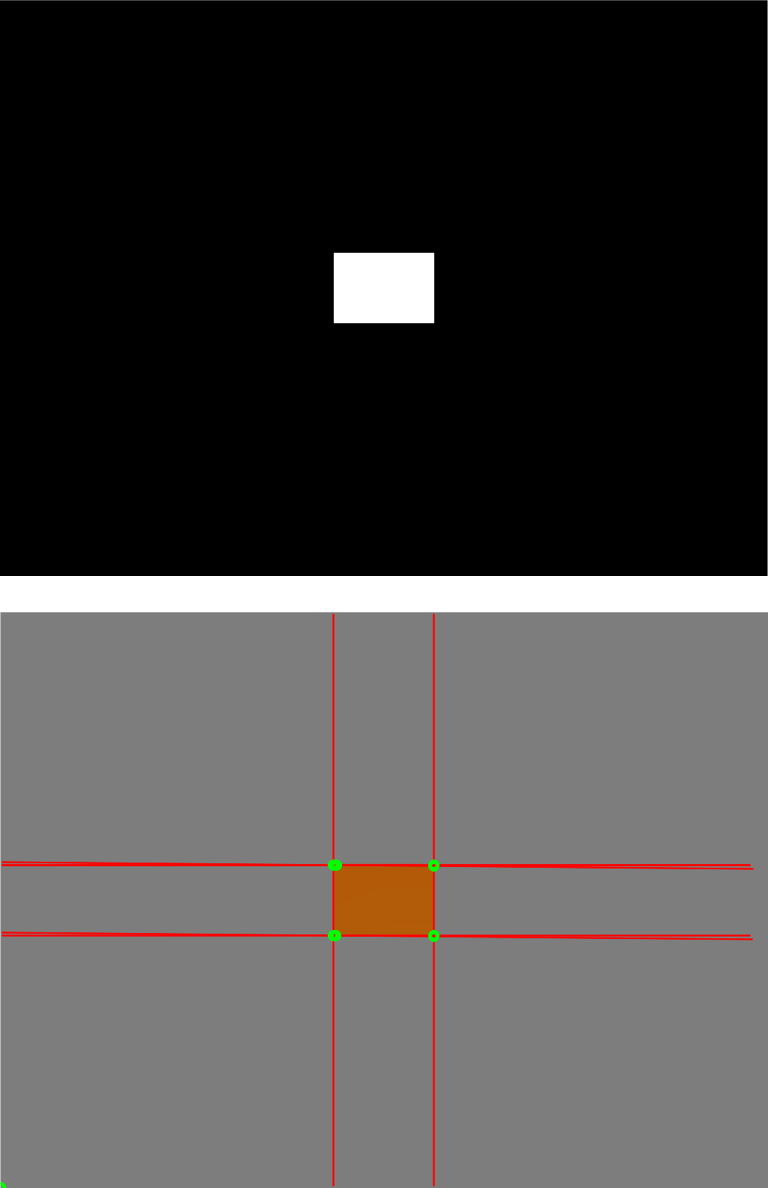
\includegraphics[width=340px]{img/rect_hough01.png}
  \caption{The correct case of rectangle detection using hough transform}
\label{rect_hough01}
\end{figure}
\begin{figure}[!ht]
  \centering
	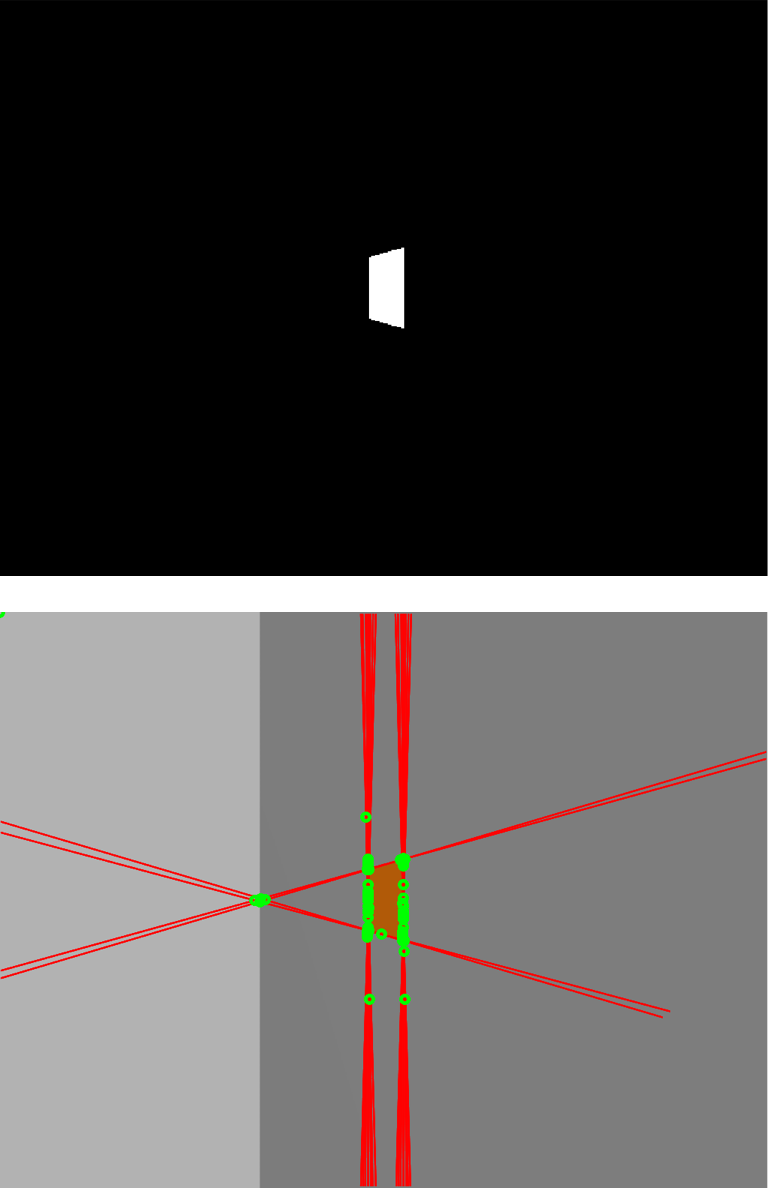
\includegraphics[width=340px]{img/rect_hough02.png}
  \caption{The failed case of rectangle detection using hough transform}
\label{rect_hough02}
\end{figure}

\begin{figure}[!ht]
  \centering
	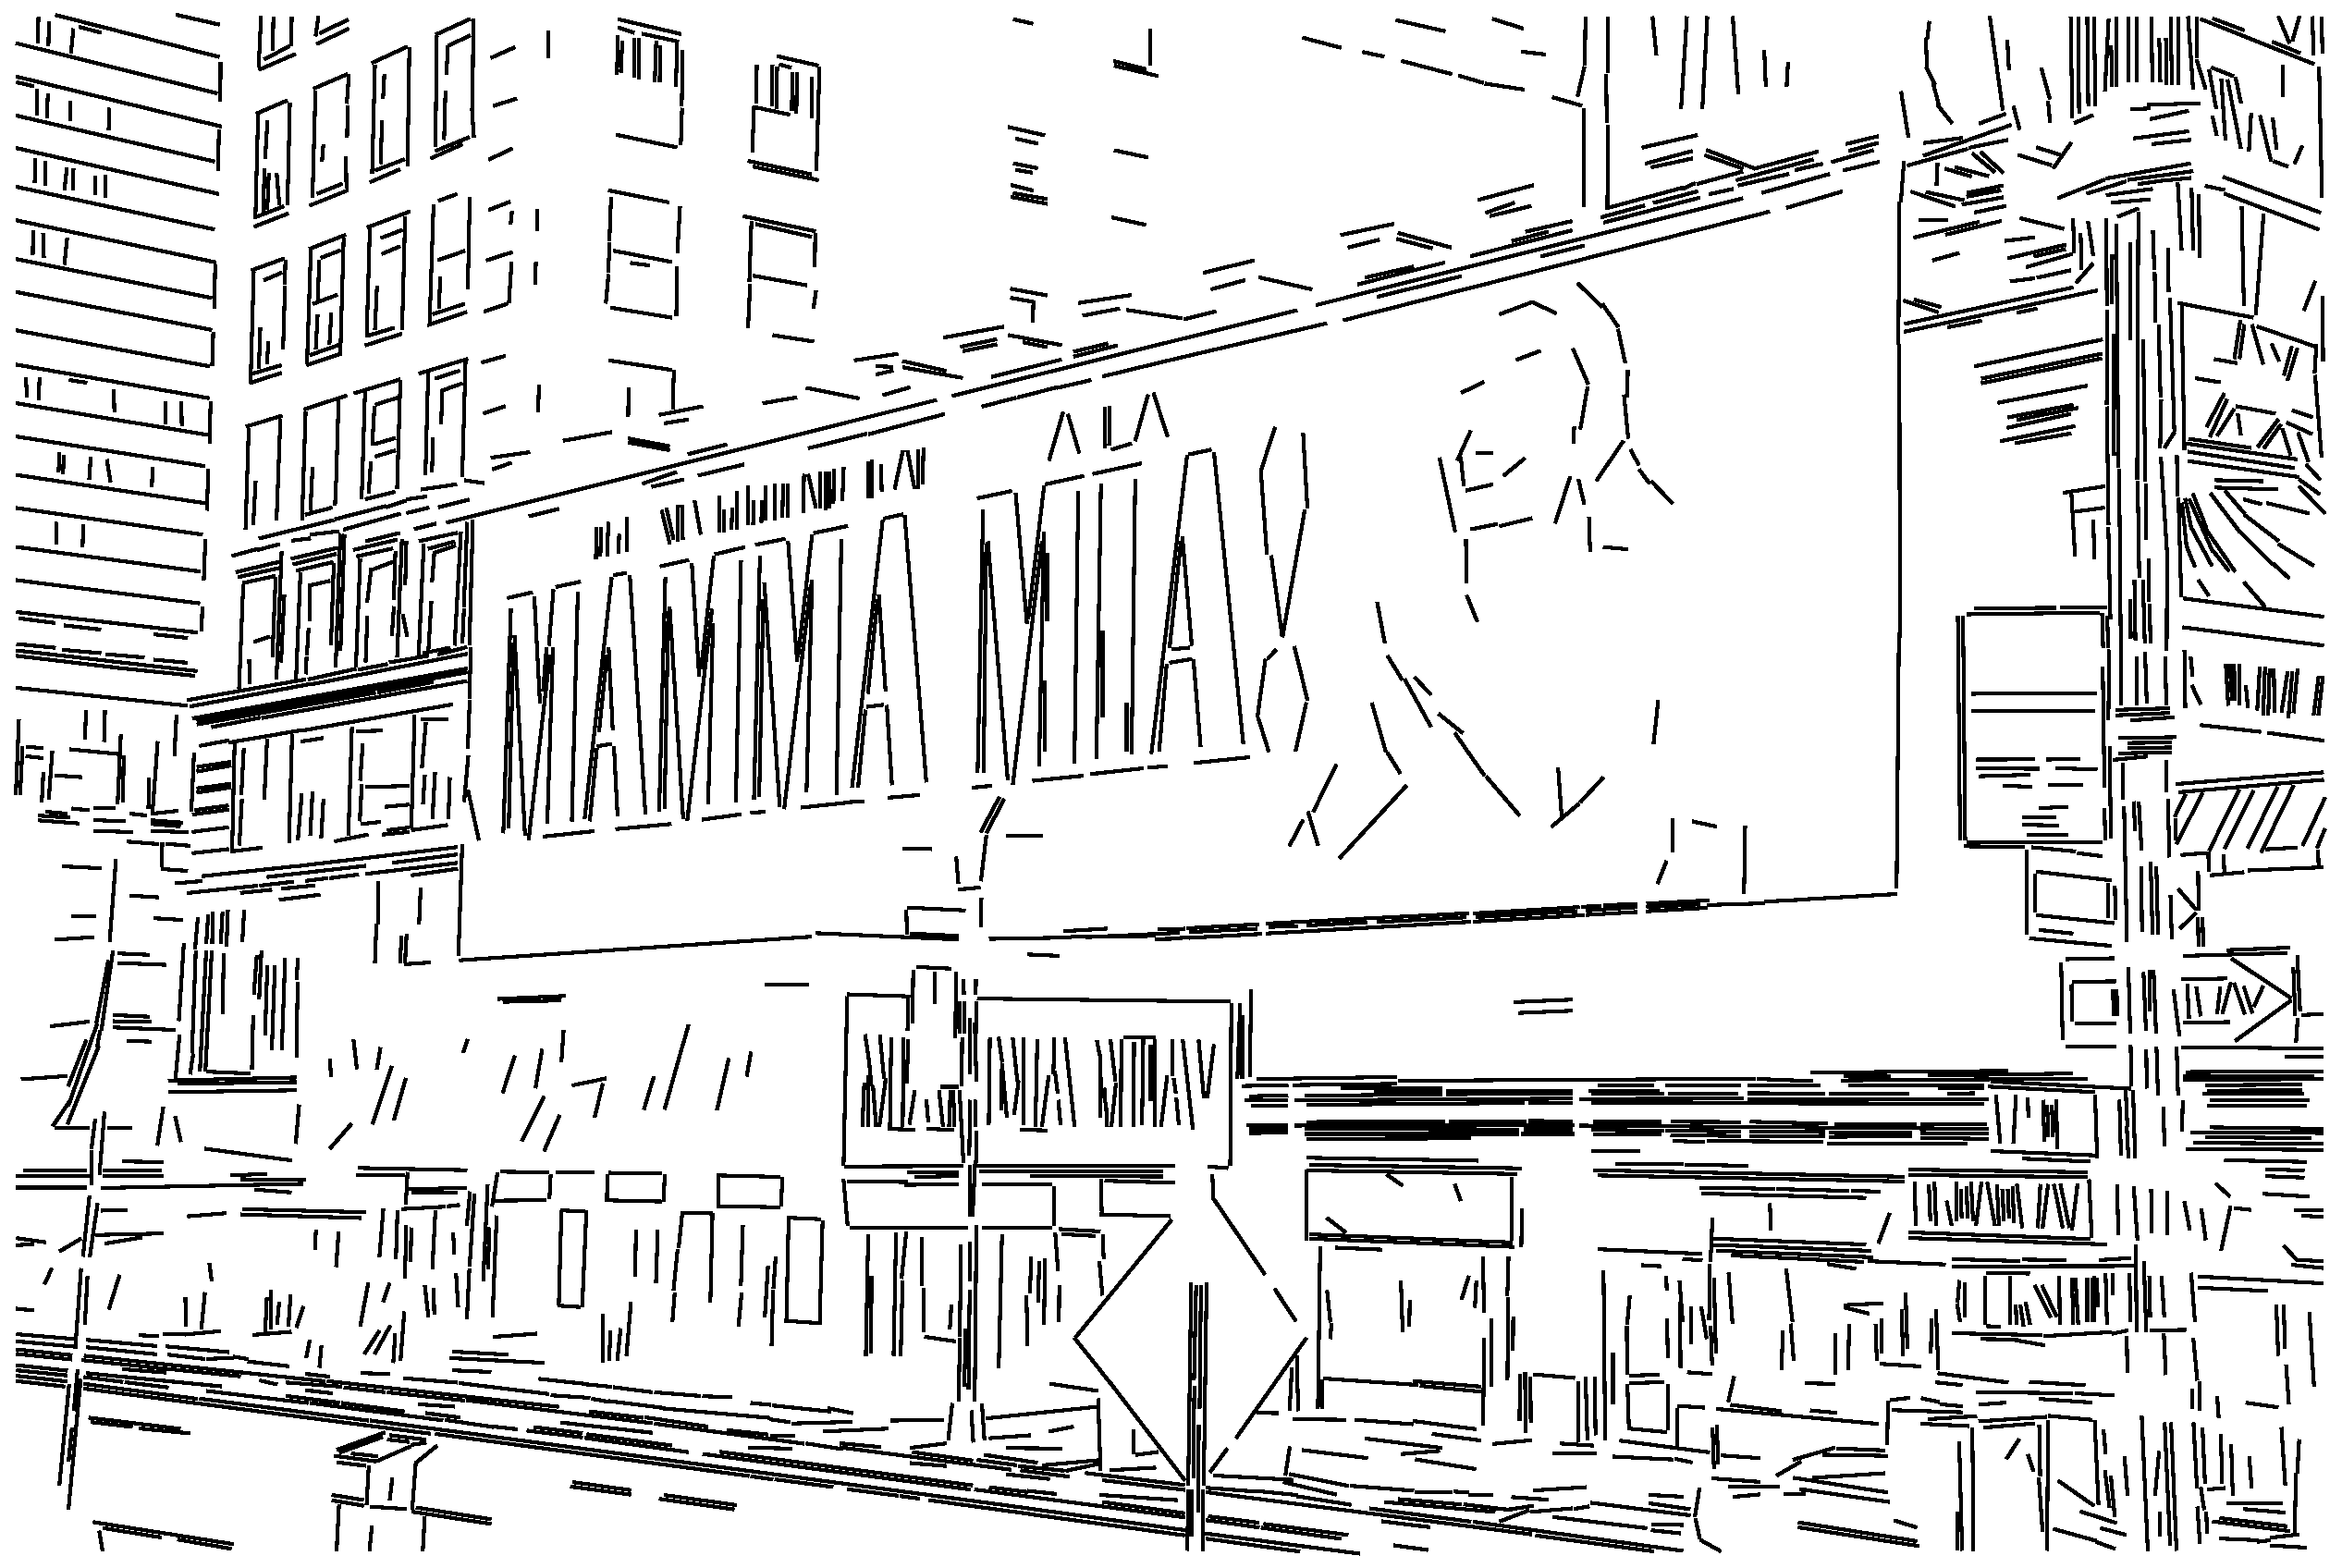
\includegraphics[width=360px]{img/BroadwayPlayers_01_lsd.eps}
  \caption{An example of line segment detection\cite{GromponeVonGioi2010} for Figure \ref{envexample} }
\label{lsdexample}
\end{figure}

 근래의 연구에서는 영상의 그래디언트를 바로 이용하여 선분을 추출하는 방법이 소개되었다\cite{GromponeVonGioi2010}. 이진화된 edge영상을 점 데이터로 간주하고 해당하던 직선 방정식을 찾던 종래의 직선 추출 방법들과는 다르게 별도의 전처리 과정 없이 직접 입력 영상을 받아 선분을 추출하며 파라미터에 민감하게 성능이 변하지 않는다는 장점이 있다. 그러나 픽셀 그래디언트를 사용하는 에지 추출 방식에 더 가까운 형태이므로 실제로는 하나의 직선이 추출되어야 하는 경우에 대해서 복수의 선분으로 쪼개져 출력되거나 일부가 검출되지 않을 수 있다. 여기서 사변형의 추출을 위해서는 선분간 연결성 확인과 사변형을 구성하지 않는 선분의 제거, 복수의 사변형이 공유하는 선분 확인 등의 기술이 추가로 필요하다. 이에 추출한 선분을 소실점, 다른 선분 간의 연관성에 따라 마르코프 랜덤 필드 모델로 선분 간의 관계를 7가지 종류의 라벨로 분류하고, 분류된 선분들의 조합으로 사각형을 구성하는 연구가 있었다\cite{Wildenauer2008}. 그러나 처리 속도가 매우 느리고 사변형을 구성하는지 여부에 대한 정보 없이 분류된 선분에서 사변형을 재구성하므로 실제 사변형이 아닌 가상의 사변형이 추출 될 여지가 있다. \\

\section{영상 영역 분할 기반의 사각형 특징 추출}
다른 방법으로 SLAM에 사용할 사각형 특징을 추출하기 위해 영역 분할 기술을 바탕으로 접근한다. 사변형에서는 선 특징보다 면 특징의 정보가 많다는 것을 주목해서 영상 이진화 방법을 반복 적용해 사변형의 후보 영역을 추출하고 영역의 경계에 대해 선분 추출을 수행하여 조건에 만족하는 선분들의 묶음을 사변형으로 간주한다. Table \ref{rect_thres}에 제안하는 방법이 서술되어 있다.
\begin{table}[!t] 
\caption{Image thresholding based rectangle detection}
\label{rect_thres}
\begin{tabular}{p{360pt}}
\toprule[1.5pt]
\textbf{Algorithm} Image thresholding based rectangle detection\\
\hline

\textbf{Input}			$I$-An image obtained by the camera, $N$-thresholding level \\
\textbf{Output}		$\{P_i\}$ - set of quadruple vertices of rectangles, $i=0,\ 1,\ ...,\ n$.
\\

\hline
\begin{algorithmic}[1]
\State Blur the image $I$ for noise reduction
\For{each color channel of the image $I$}
\For{$i=0,1, ..., N$}
\If {i=0}
	\State Detect edge with canny edge detector
\Else
	\State Do image thresholding with threshold $255/N\times i$ for an image $I$
\EndIf
	\State Find a set of contours $C=\{ c_0, c_1, ..., c_j \}$ using chain code method in an thresholded image.
	\For {each contour $c_k$}
		\State Find a set of connected line segments $L$ in the contour $c_k$ using split-and-merge method.
		\If { the number of elements in $L$ = 4 and satisfying convexity}
			Add corresponded end points of line segments as quadrilateral in $P_i$
		\EndIf
	\EndFor
\EndFor
\EndFor
\end{algorithmic}\\
\toprule[1.5pt]
\end{tabular}
\end{table}
이 방법은 색상 채널에서의 이진화를 응용하여 사각형을 검출한다. 한 사변형의 내부 픽셀은 서로 유사한 시각적 형태와 색상을 가진다는 가정을 두고 이진화의 임계치를 정해진 단계씩 변경하며 영상을 처리한다. 이진화된 이미지는 chain code 방법을 통해 윤곽선이 추출되고, split-and-merge 방법\cite{Douglas1973}을 이용하여 윤곽선에서 선분을 검출한다. 검출된 선분이 4개이고 사변형으로서 가져야 할 성질을 만족하면 사변형으로 저장하는 것을 매 이진화 처리 이후 수행하여 가능한 사변형을 모두 검출한다. canny edge 검출기를 사용하여 edge 영상 위에서 선분을 추출하고 사각형을 확인하는 과정을 더해 이전 장에 서술한 직선 추출 기반 사각형 검출 방법을 일부 도입하여 성능의 향상을 꾀하였다.
단계적 이진화를 이용한 영상 영역 분할 방법을 사용하여 사각형을 추출하였으므로 영상 이진화의 결과에 따라 영상 전체가 사각형으로 검출되거나 혹은 특징으로 사용할 수 없을 정도로 작은 크기의 사각형이 검출 될 수도 있다. 이는 SLAM의 특징으로 사용하기에는 문제가 있는 검출 결과이므로 필요에 따라 이러한 결과를 억제할 수 있는 방안을 검토해야 한다.
\begin{figure}[!ht]
  \centering
	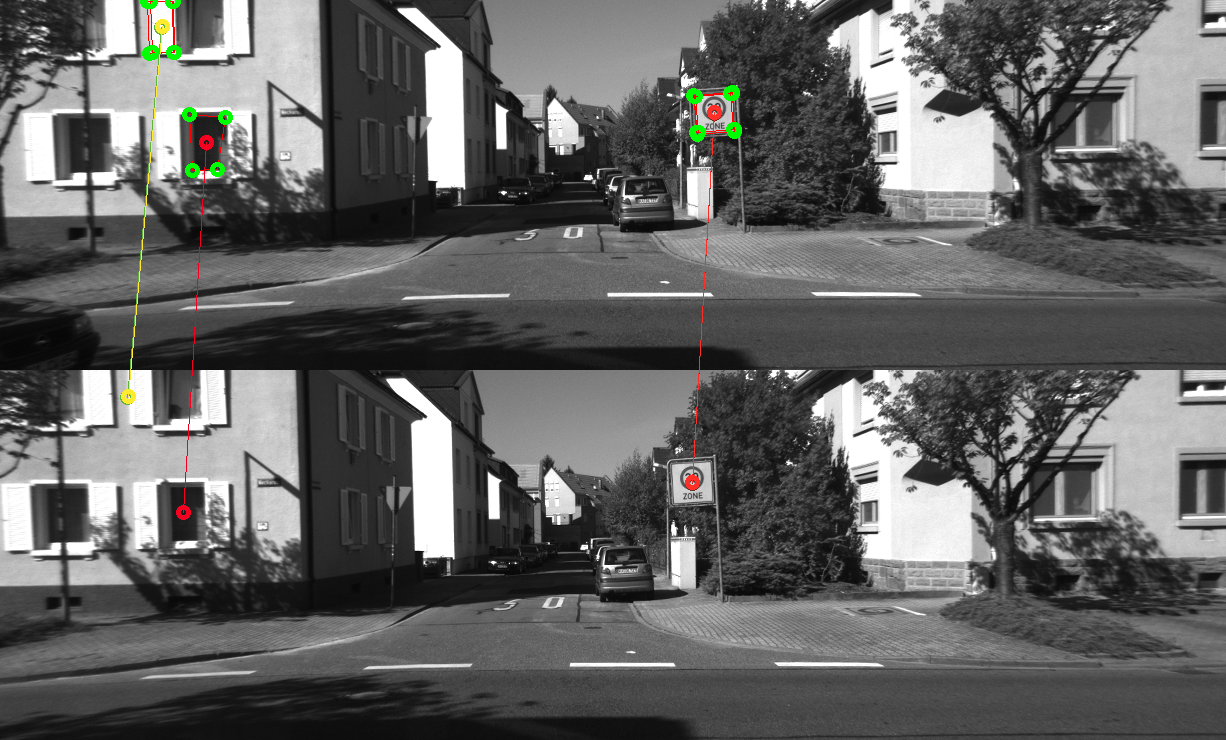
\includegraphics[width=360px]{img/rect_seg.png}
  \caption{An example of extracting quadrilateral in an outdoor scene }
\label{segment_example}
\end{figure}
%%%%%%%%%%%%%%%%%%%%%%%%%%%%%%%%%%%%%%%%%%%%%%%%%%%%%%%%%%%%%%%%%%%%%%%%%%%%%%%%%%%%%%%%%%%%%%%%%%%%%%%%%%%%%%%%%%%
%%%%%%%%%%%%%%%%%%%%%%%%%%%%%%%%%%%%%%%%%%%%%%%%%%%%%%%%%%%%%%%%%%%%%%%%%%%%%%%%%%%%%%%%%%%%%%%%%%%%%%%%%%%%%%%%%%%
%%%%%%%%%%%%%%%%%%%%%%%%%%%%%%%%%%%%%%%%%%%%%%%%%%%%%%%%%%%%%%%%%%%%%%%%%%%%%%%%%%%%%%%%%%%%%%%%%%%%%%%%%%%%%%%%%%%
%\chapter{사각형 특징을 위한 특징 기술자}
%일반적인 점 특징이 특징 기술자로 점 근방의 국소 패치를 가공하여 이용하는 것에 비해 사각형은 특징의 내부에 특징 기술자로서 사용될 수 있는 정보가 다수 포함되어 있다. 특징 추출 시 사각형의 네 꼭지점은 같은 평면 상에 위치하는 것을 가정했고 선분카메라쌍 방법을 이용하여 직사각형의 종횡비 또한 복원할 수 있다. 특징과 직접적인 연관이 있는 정보인지 구별하지 못하고 무조건 고정된 크기와 범위의 영역만을 사용하는 점 특징 기반의 특징 기술자와는 다르게 제안하고자 하는 사각형 특징을 위한 특징 기술자는 추출한 사각형의 내부가 모두 특징과 직접적으로 관련된 정보를 담고 있으며, 특징 기술자의 크기 또한 복원한 사각형의 크기나 정보량에 따라 가변적으로 조절할 수 있는 여지를 가지고 있다. \\
%Figure \ref{envexample}로 예를 들면 직사각형으로 추출되는 시각 특징 중 포스터, 간판, 교통 표지판, 게시판 등은 사각형 내부에 그래디언트 정보가 위치별로 다양하게 분포되어 있어 특징 기술자로서 많은 정보를 가질 수 있다. 그러나 건물 외벽, 타일, 창문, 빈 종이 등은 사각형 내부가 일정한 패턴으로 이루어져있어 상대적으로 위치에 대한 그래디언트 변화가 적다. 이에 이들을 같은 구조의 기술자로 구분하기 위해 색상정보와 그래디언트 정보를 융합한 특징 기술자를 제안한다.\\
%CIELAB
%luminance channel에서 hog
%AB채널에서 컬러 히스토그램 매칭
%%%%%%%%%%%%%%%%%%%%%%%%%%%%%%%%%%%%%%%%%%%%%%%%%%%%%%%%%%%%%%%%%%%%%%%%%%%%%%%%%%%%%%%%%%%%%%%%%%%%%%%%%%%%%%%%%%%
%%%%%%%%%%%%%%%%%%%%%%%%%%%%%%%%%%%%%%%%%%%%%%%%%%%%%%%%%%%%%%%%%%%%%%%%%%%%%%%%%%%%%%%%%%%%%%%%%%%%%%%%%%%%%%%%%%%
%%%%%%%%%%%%%%%%%%%%%%%%%%%%%%%%%%%%%%%%%%%%%%%%%%%%%%%%%%%%%%%%%%%%%%%%%%%%%%%%%%%%%%%%%%%%%%%%%%%%%%%%%%%%%%%%%%%
\chapter{실험결과}
\section{선분카메라쌍 기반의 자세 추정 성능 실험}
이 장에서는 선분카메라쌍을 이용하여 사각형 특징으로부터 카메라의 상대 자세를 복원하는 방법의 정량적인 성능을 분석한다. 유효한 기준치를 얻기 위해 Gazebo 시뮬레이터를 이용하여 사각형과 카메라를 묘사하고 실험을 수행하였다. 시뮬레이터 환경에서는 카메라가 전역 중심 좌표계를 기준으로 경위도식 움직임을 할 수 있도록 구성되어 있다. 실험에 사용한 카메라는 640*480의 해상도와 100도의 화각을 가지고 있고 baseline이 120mm인 스테레오 카메라이다. 촬영하는 사각형은 가로 210mm, 세로 297mm의 크기를 가지고 있고, 사각형은 전역 기준 좌표계의 xy평면 위에서 움직인다. 시뮬레이터의 구성은 figure \ref{gazebo}에서 확인할 수 있다.
\begin{figure}[!ht]
  \centering
	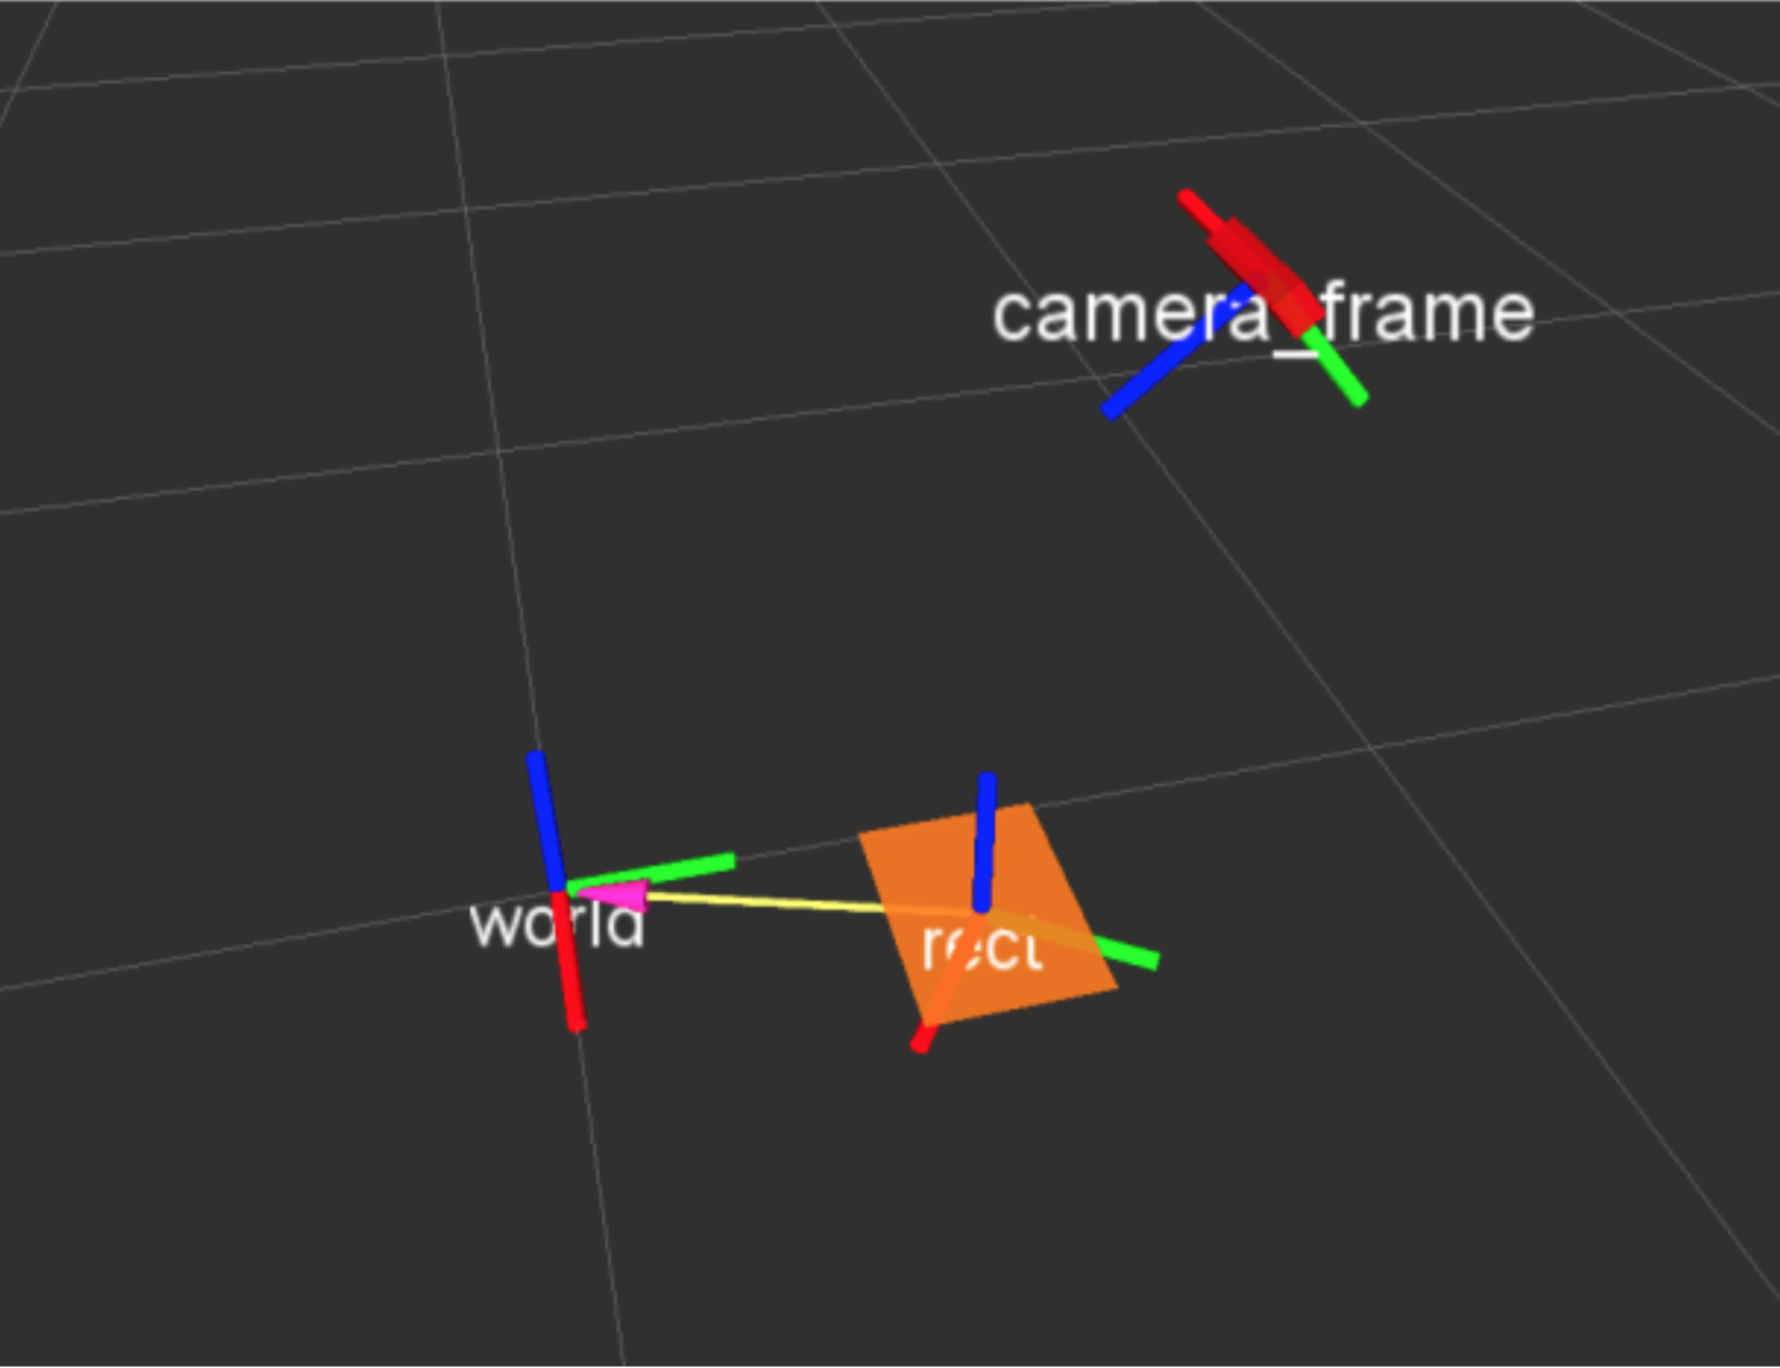
\includegraphics[width=360px]{img/gazebo.png}
  \caption{The configuration of the camera and the rectangle feature for simulation }
\label{gazebo}
\end{figure}
 이에 선분카메라쌍 알고리즘을 통해 사각형 특징과 카메라간의 상대 위치 추정을 할 때 오차를 분석하기 위해 두 가지 실험을 구성하였다. 첫 번째 실험은 회전에 대한 성능을 분석하기 위해 경위대의 위도와 거리를 각각 0.7 rad, 1 m로 고정하고 경도를 0.4 rad부터 0.1 rad씩 6 rad까지 회전하는 실험을 구성하였다. Figure \ref{pose_yz}, \ref{pose_xy}, \ref{pose_zx}에 위 실험에서 선분카메라쌍 방법으로 구한 상대 위치와 ground truth를 공간상에 표현하고 x, y, z축을 기준으로 투영해서 보여주고 있다. Figure \ref{X_ang}, \ref{Y_ang}, \ref{Z_ang}에서는 회전 변화에 대한 두 값의 차이를 정량적으로 분석하기 위해 경위도의 변화에 따른 추정값과 ground truth를 비교하고 있다. 이 때 선분카메라쌍 방밥을 이용한 추정치가 $\frac{n\pi}{2}( n=1,2,3,\dots)$근방에서 계산되지 않은 것을 볼 수 있다. 이는 선분카메라쌍 알고리즘의 입력이 사다리꼴일 경우(사변형을 이루는 두 선분이 평행인 경우) 발생하는 문제로, 이미지 평면은 카메라의 픽셀에 맞추어 양자화되어 실제로 평행하지 않은 투영 사변형도 평행한 것으로 간주되어 위와 같은 문제가 발생한다. Figure \ref{RMS_ang}에서는 회전 변화에 대한 추정치의 RMS오차를 보여준다. 오차는 모든 실험 결과에 대해 0.05rad이하로 발생하였으며 불연속점 근방에서 비교적 큰 오차를 보이거나 아주 작은 오차를 보이는 것을 확인할 수 있었다. 이러한 오차 양상의 원인을 분석해보기 위해 Figure \ref{ca_ang}에서는 선분카메라쌍 기반 사각형 복원 방법의 결과물인 사각형 종횡비 복원 값을 회전 변환에 대해 출력하고 있다. 위아래를 구분할 수 없는 직사각형은 세로가 긴 형태 또는 가로가 긴 형태를 서로 구분할 수 없어 종횡비는 $\frac{\pi}{2}$ 기준으로 대칭성을 가진다고 볼 수 있다. 이 실험에서도 직사각형의 형태만이 추출되므로 두 개의 종횡비가 추출될 수 있다. 실험 결과는 불연속점을 기준으로 종횡비의 값이 바뀌고 상대적으로 큰 오차를 보이고 있어 사각형 복원 성능이 자세 추출 성능에 중요한 영향을 미치고 있음을 확인할 수 있었다.
 두 번째 실험은 거리에 대한 성능을 분석하기 위해 두 물체 사이의 거리를 0.5 m부터 5.5 m까지 0.1 m씩 증가하며 자세추정 결과를 확인하였다. 위의 실험 분석과 유사하게 figure \ref{X_d}, \ref{Y_d}, \ref{Z_d}에서는 실제 사각형과 카메라 간의 상대 위치와 제안하는 방법을 이용하여 추정한 결과를 비교하였고 figure \ref{RMS_d}, \ref{ca_d}에서는 각각 거리에 따른 RMS오차와 사각형 복원 방법의 종횡비 추출 결과를 출력하였다. 실험 구간에서 추정한 종횡비가 약 0.04rad감소함에 따라 RMS 오차는 0.007m까지 증가하는 것을 확인 할 수 있다. \\
이와 같은 결과에 따라 사각형 추출이 올바르게 이루어 질 경우 정밀하게 특징과 카메라간 상대 자세를 추정할 수 있음을 실험적으로 보였다.
\begin{figure}[!ht]
  \centering
	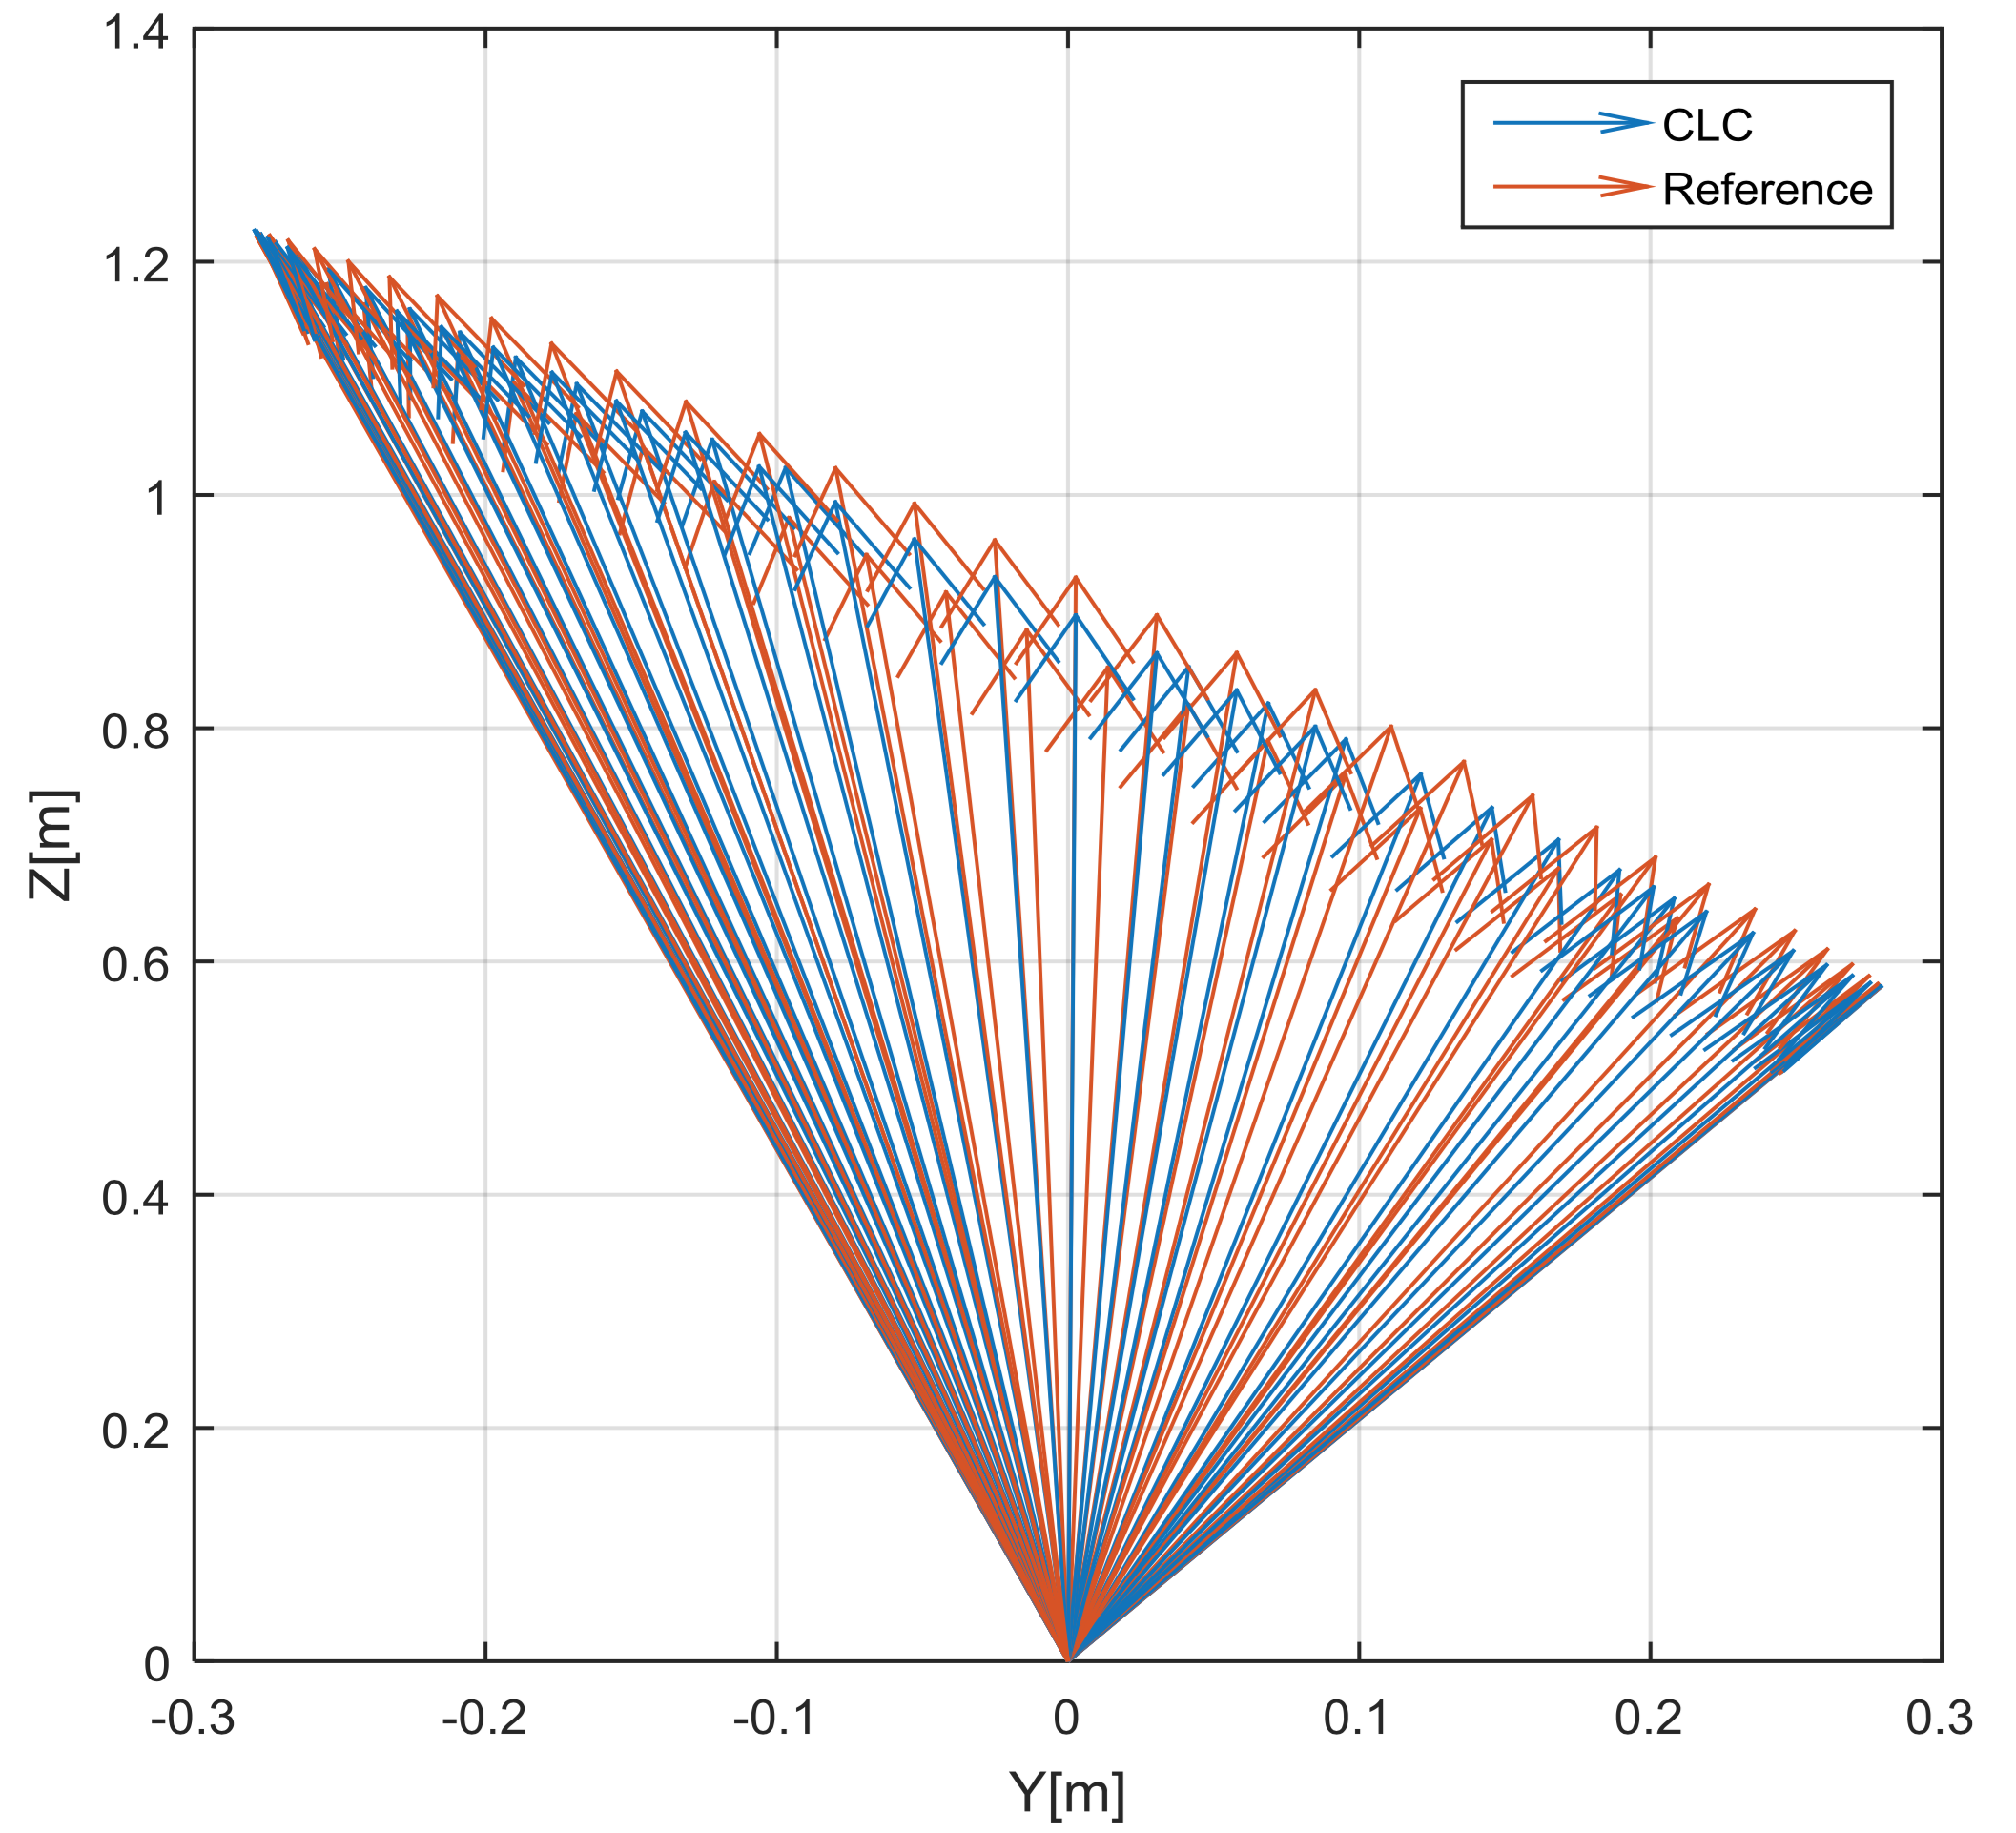
\includegraphics[width=360px]{img/pose_yz.png}
  \caption{The result of the proposed method and reference pose with respect to distance and YZ-plane }
\label{pose_yz}
\end{figure}
\begin{figure}[!ht]
  \centering
	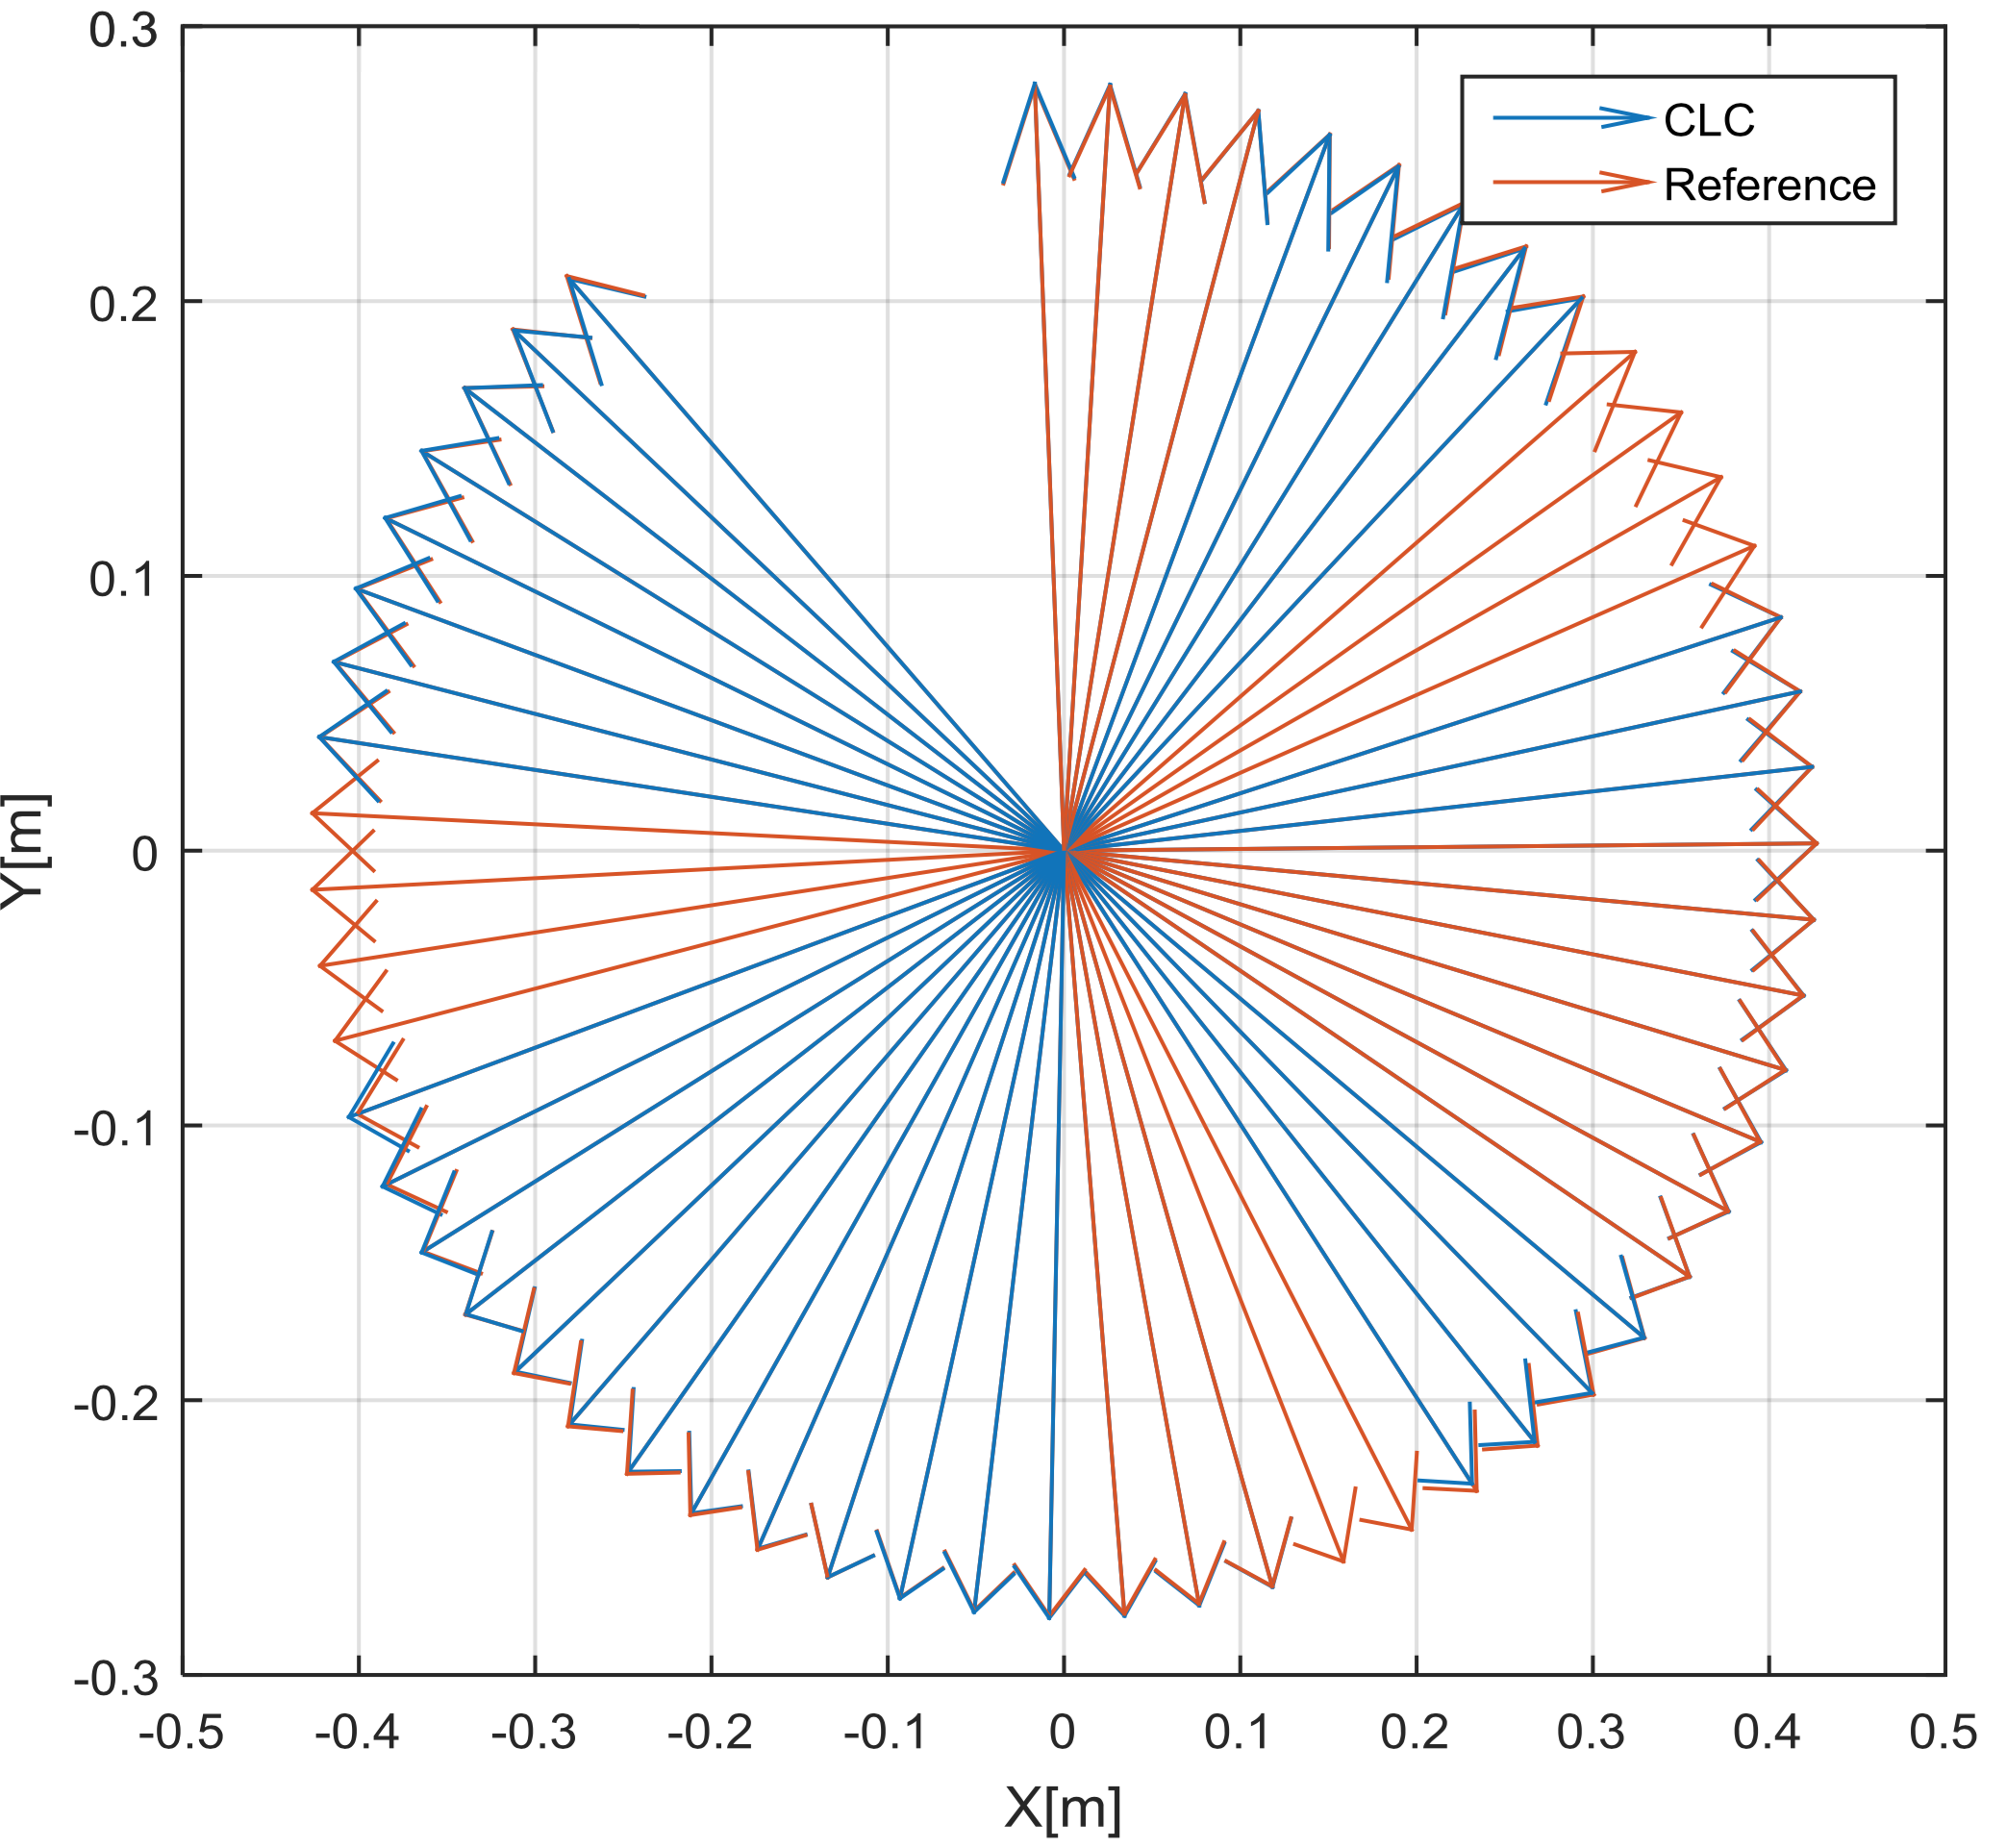
\includegraphics[width=360px]{img/pose_yx.png}
  \caption{The result of the proposed method and reference pose with respect to distance and XY-plane }
\label{pose_xy}
\end{figure}
\begin{figure}[!ht]
  \centering
	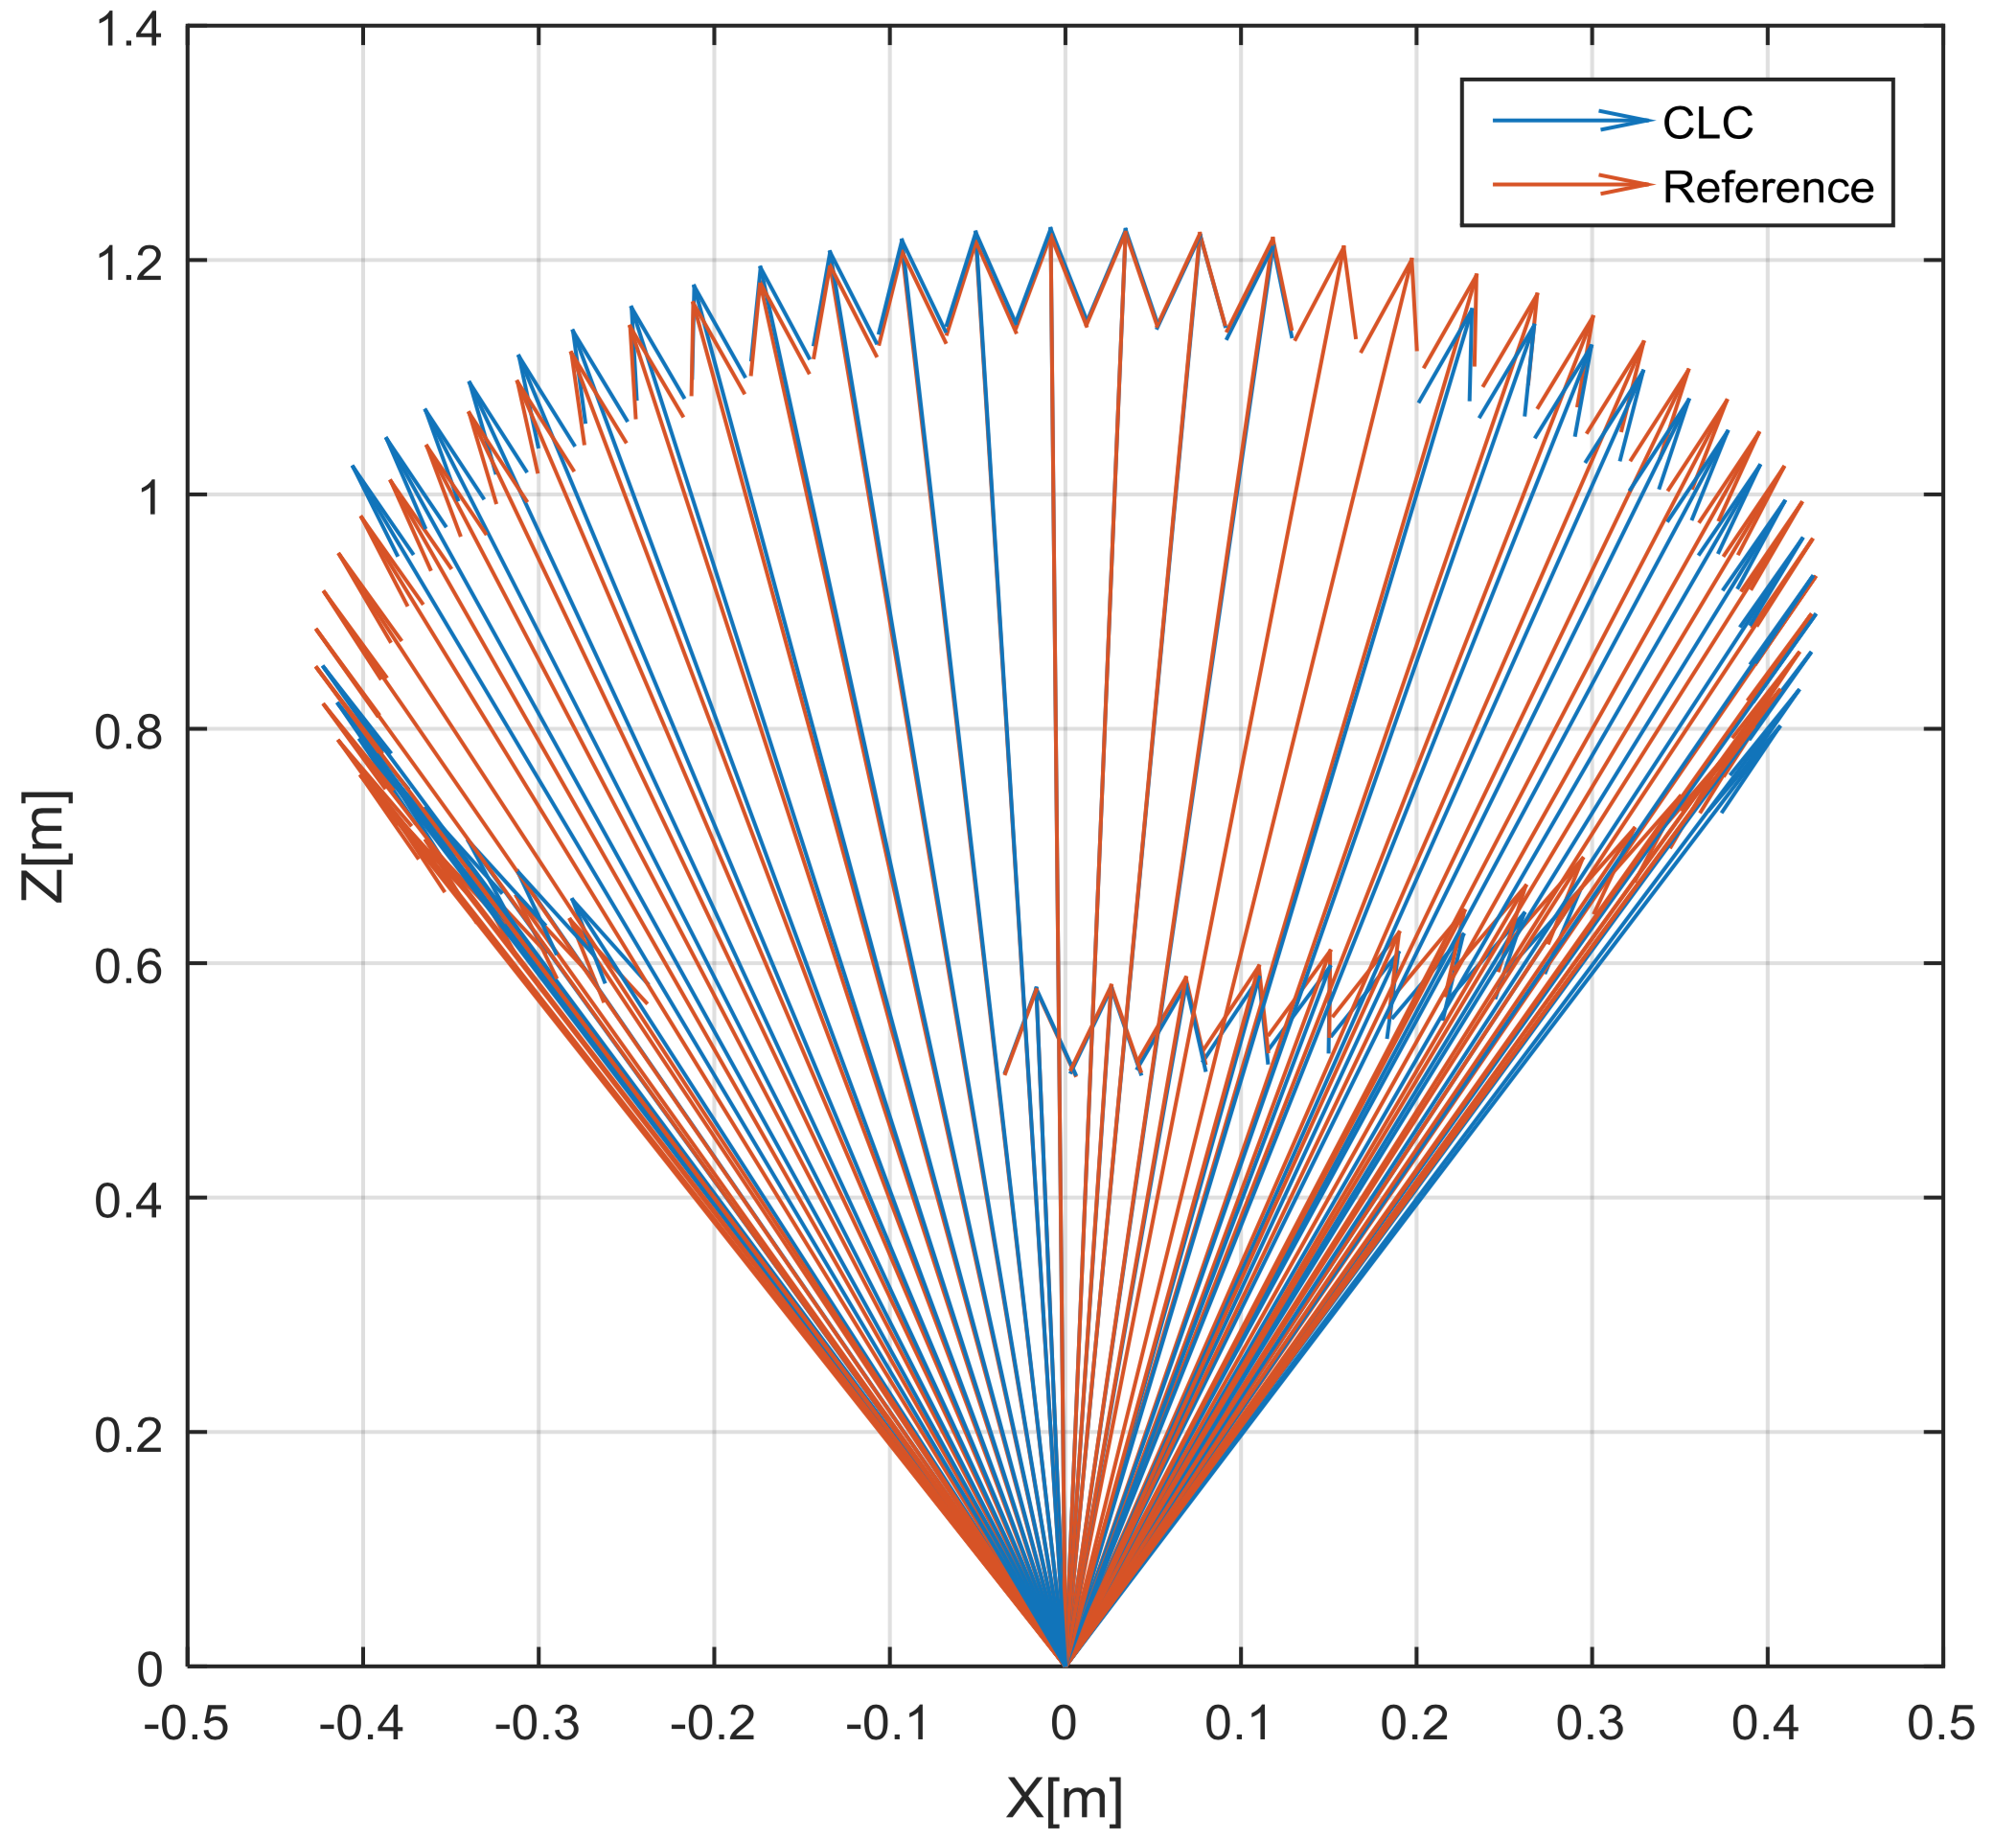
\includegraphics[width=360px]{img/pose_zx.png}
  \caption{The result of the proposed method and reference pose with respect to distance and XZ-plane }
\label{pose_zx}
\end{figure}


\begin{figure}[!ht]
  \centering
	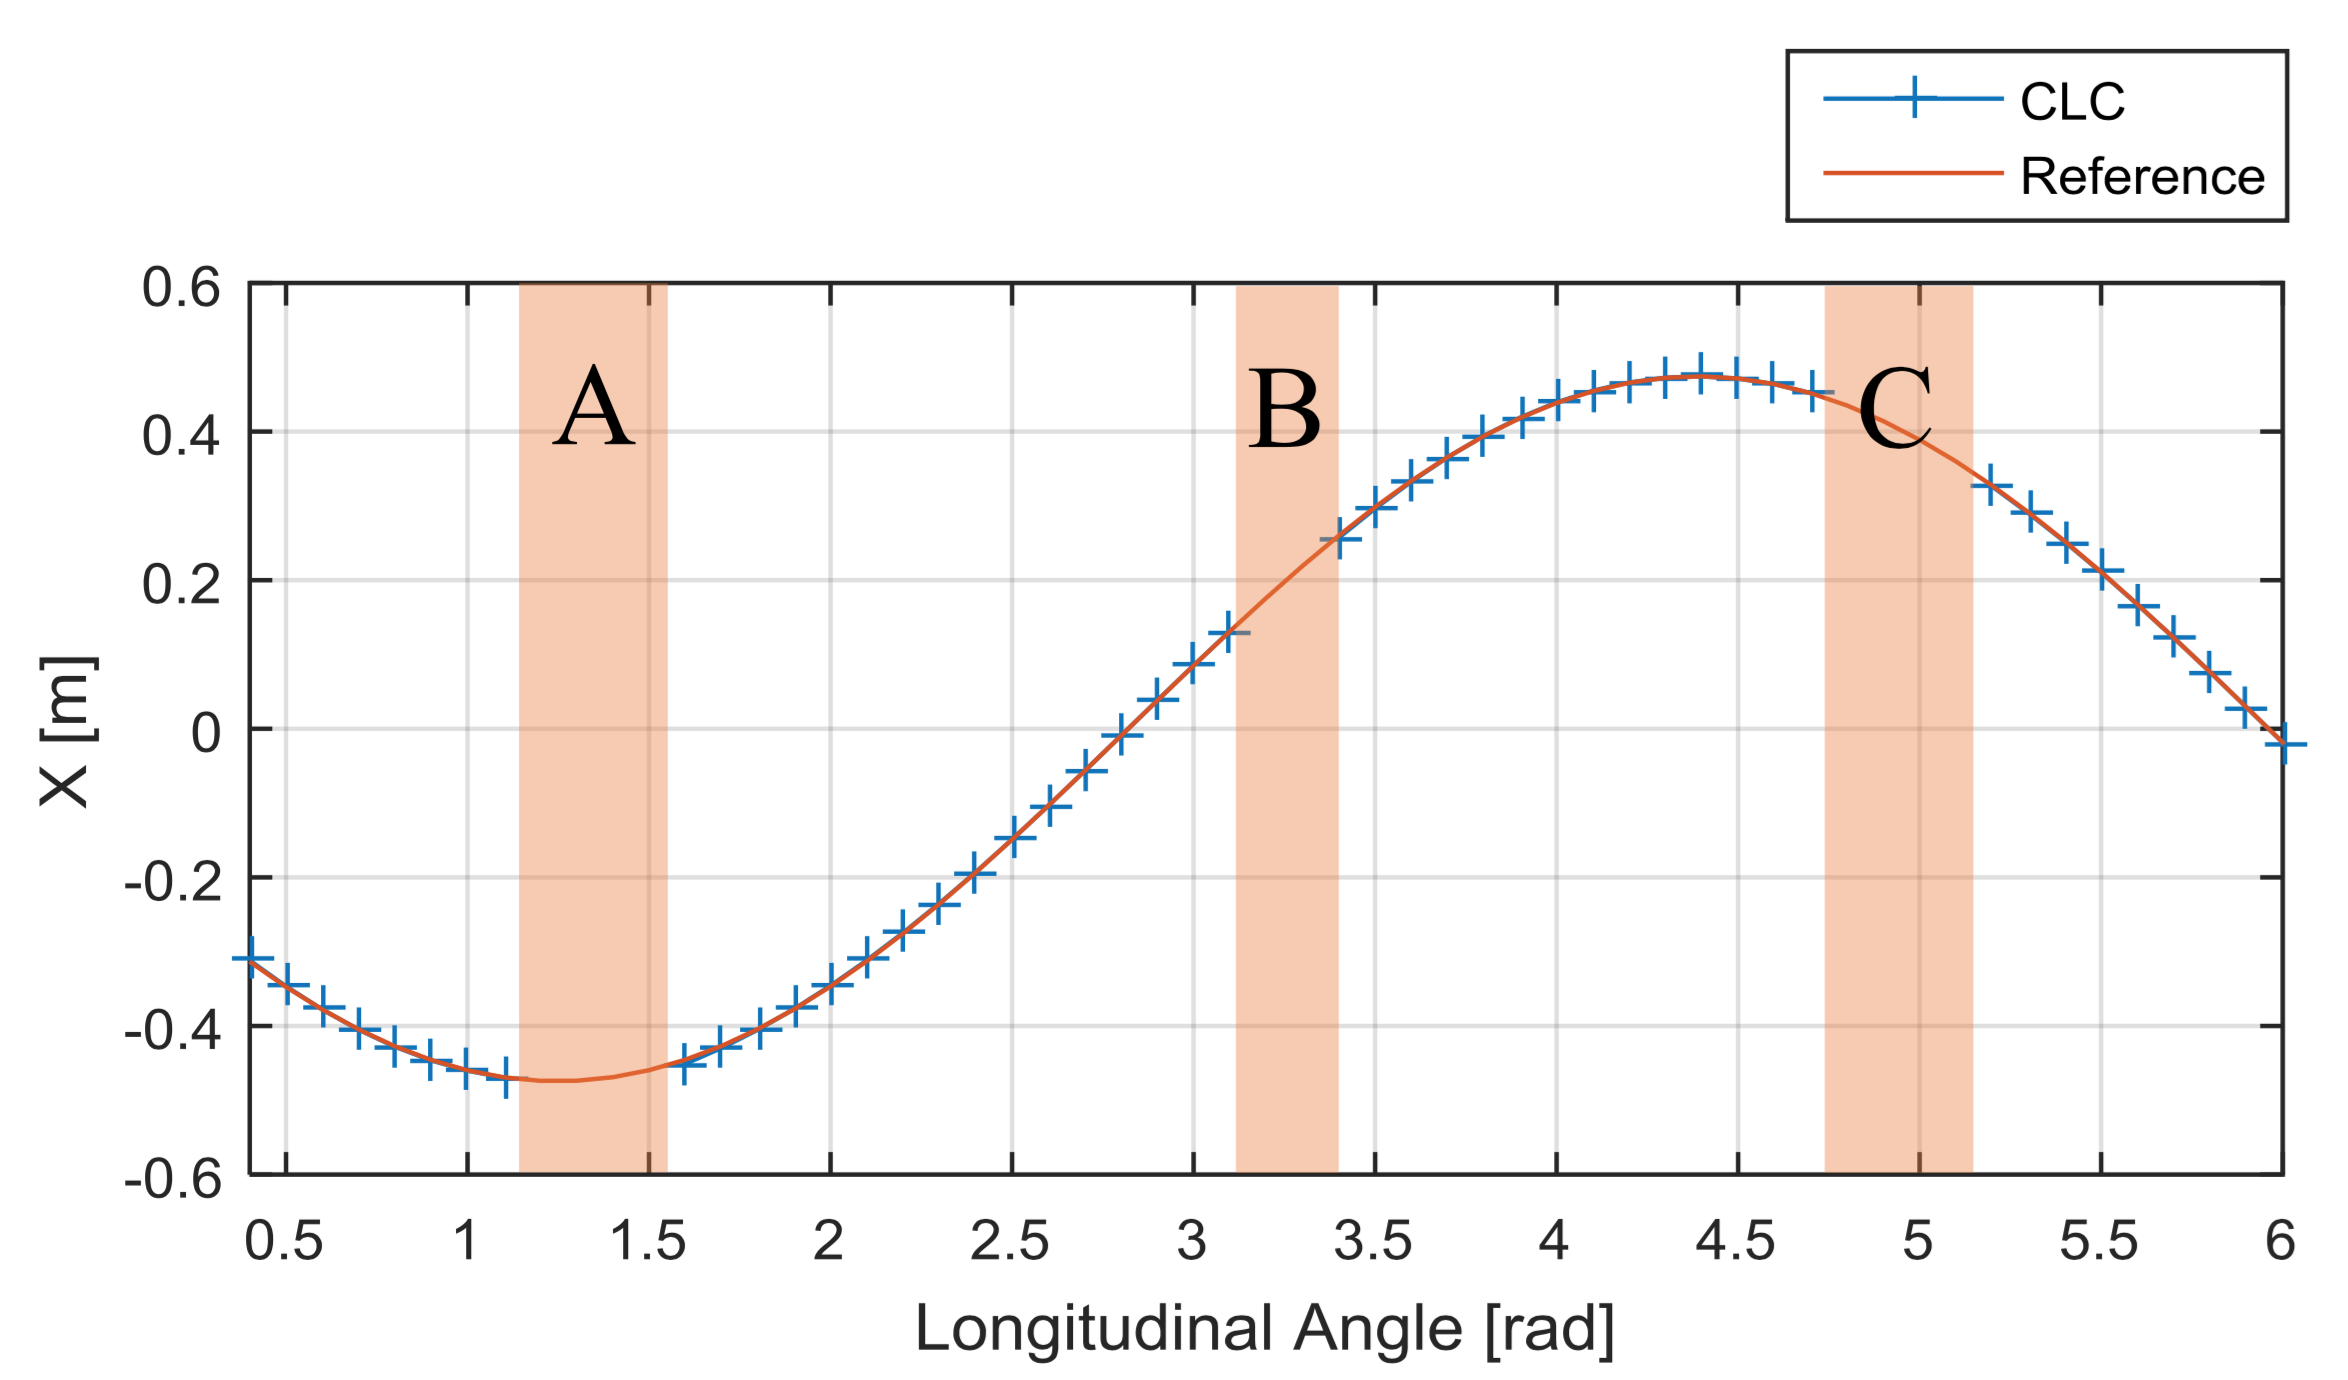
\includegraphics[width=360px]{img/X_ang.png}
  \caption{The result of the proposed method and reference pose with respect to longitudinal angle and X-axis }
\label{X_ang}
\end{figure}
\begin{figure}[!ht]
  \centering
	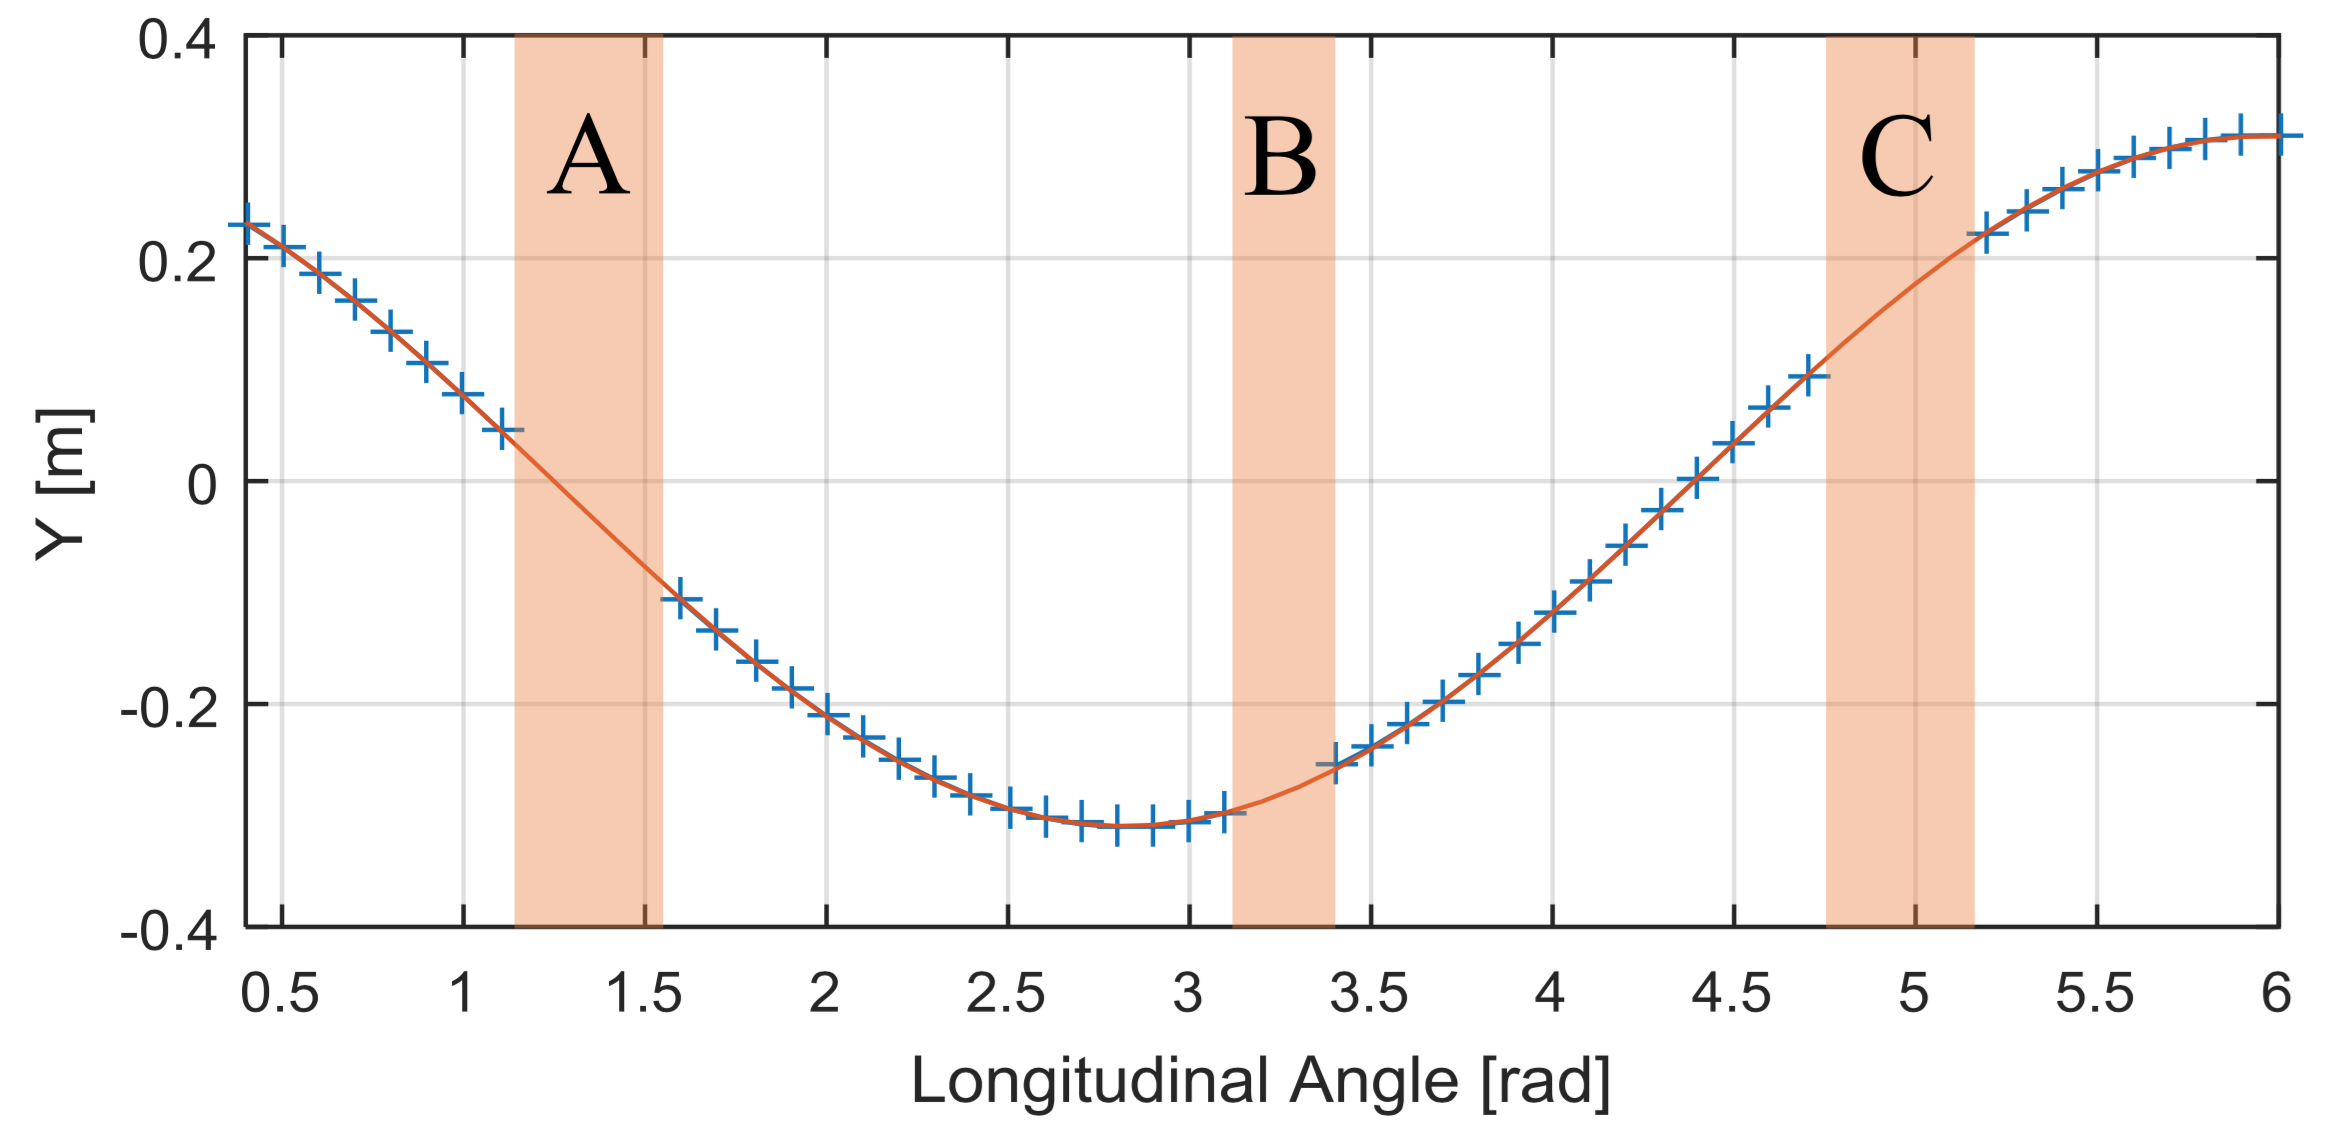
\includegraphics[width=360px]{img/Y_ang.png}
  \caption{The result of the proposed method and reference pose with respect to longitudinal angle and Y-axis }
\label{Y_ang}
\end{figure}
\begin{figure}[!ht]
  \centering
	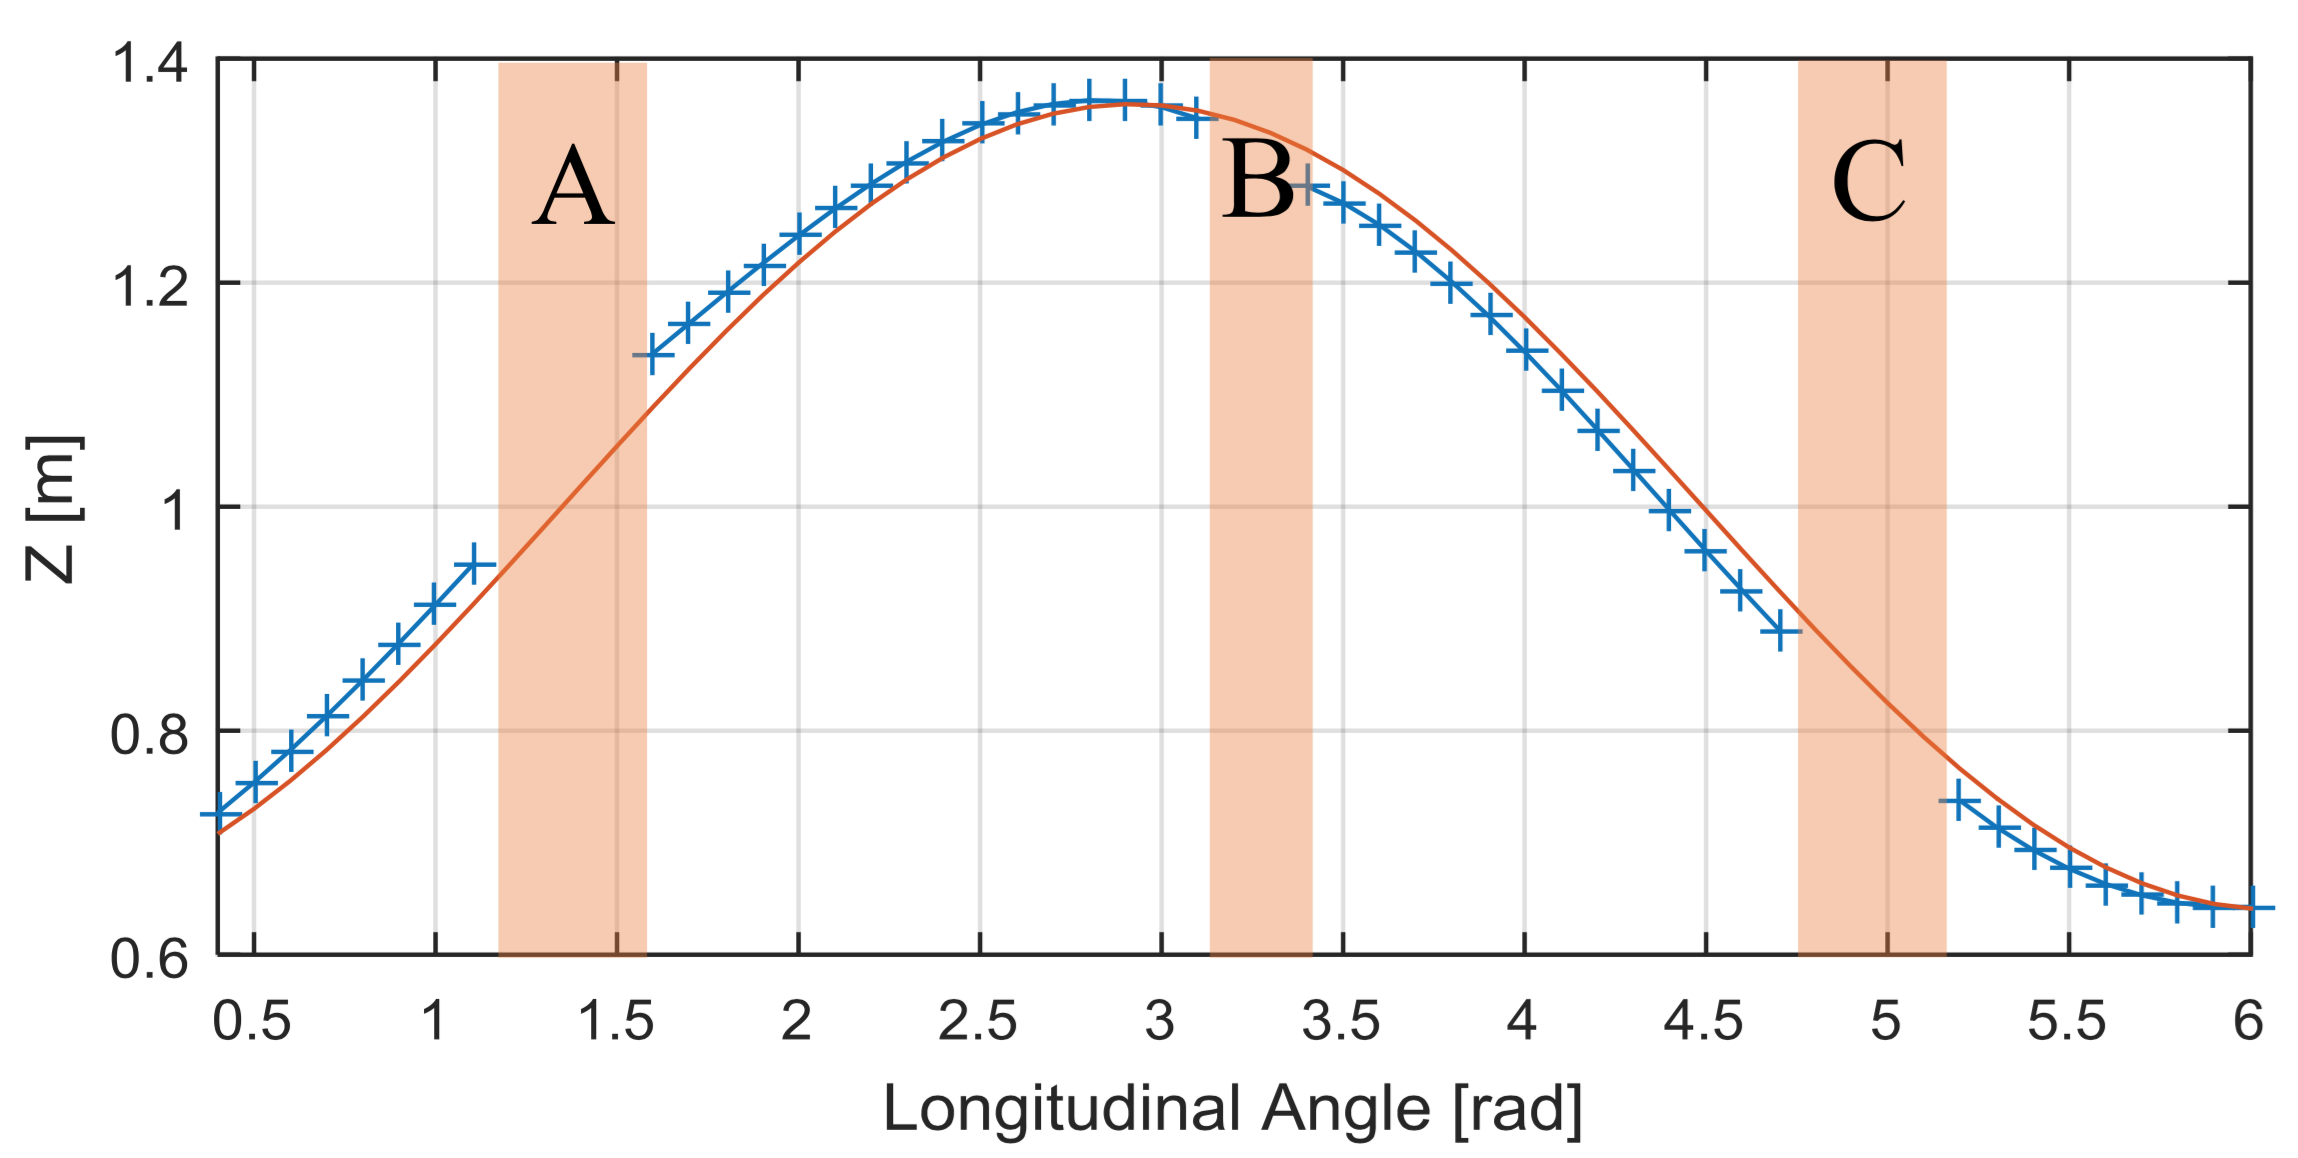
\includegraphics[width=360px]{img/Z_ang.png}
  \caption{The result of the proposed method and reference pose with respect to longitudinal angle and Z-axis }
\label{Z_ang}
\end{figure}
\begin{figure}[!ht]
  \centering
	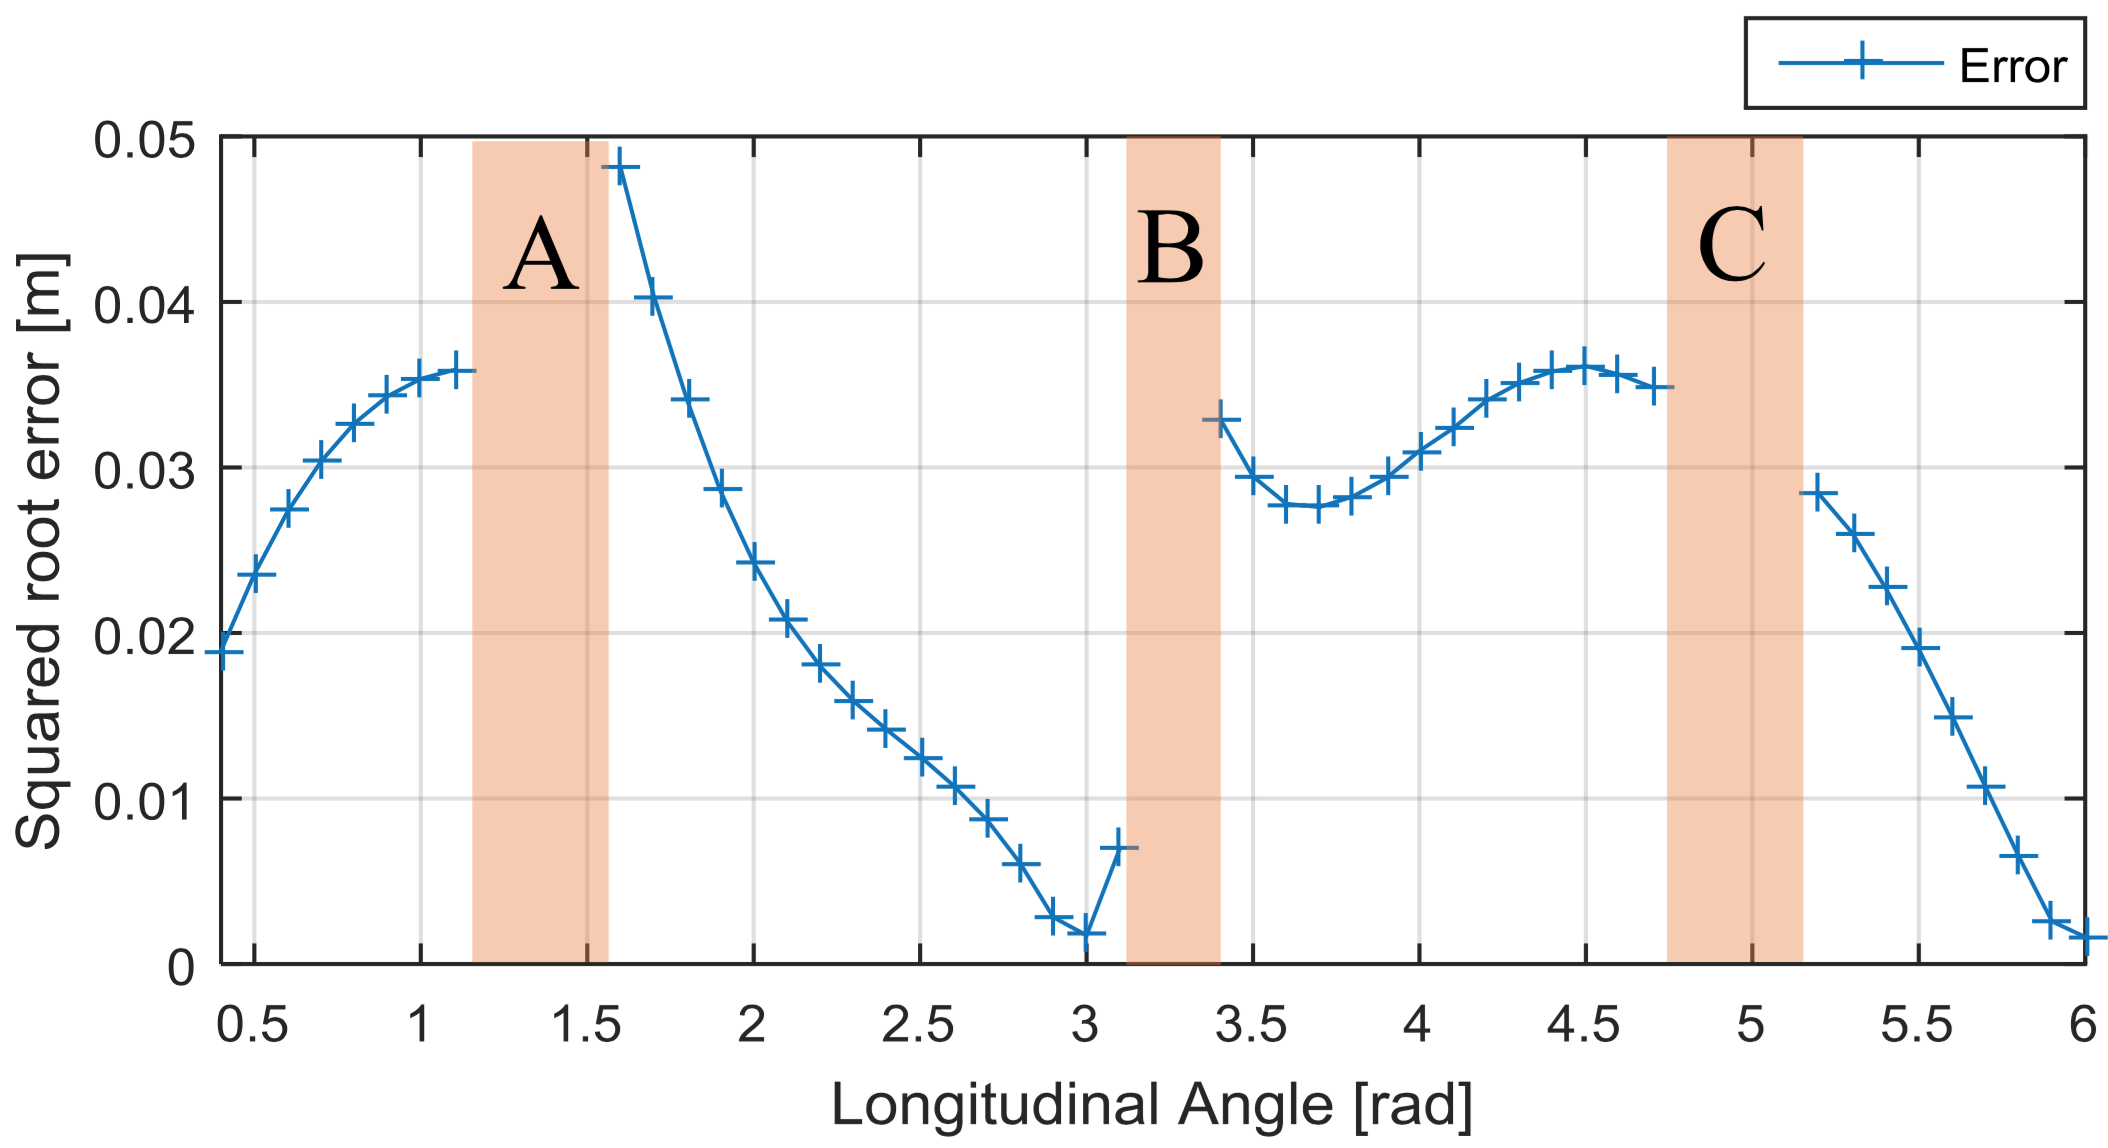
\includegraphics[width=360px]{img/RMS_ang.png}
  \caption{The square root error of the proposed pose estimation method with respect to longitudinal angle}
\label{RMS_ang}
\end{figure}
\begin{figure}[!ht]
  \centering
	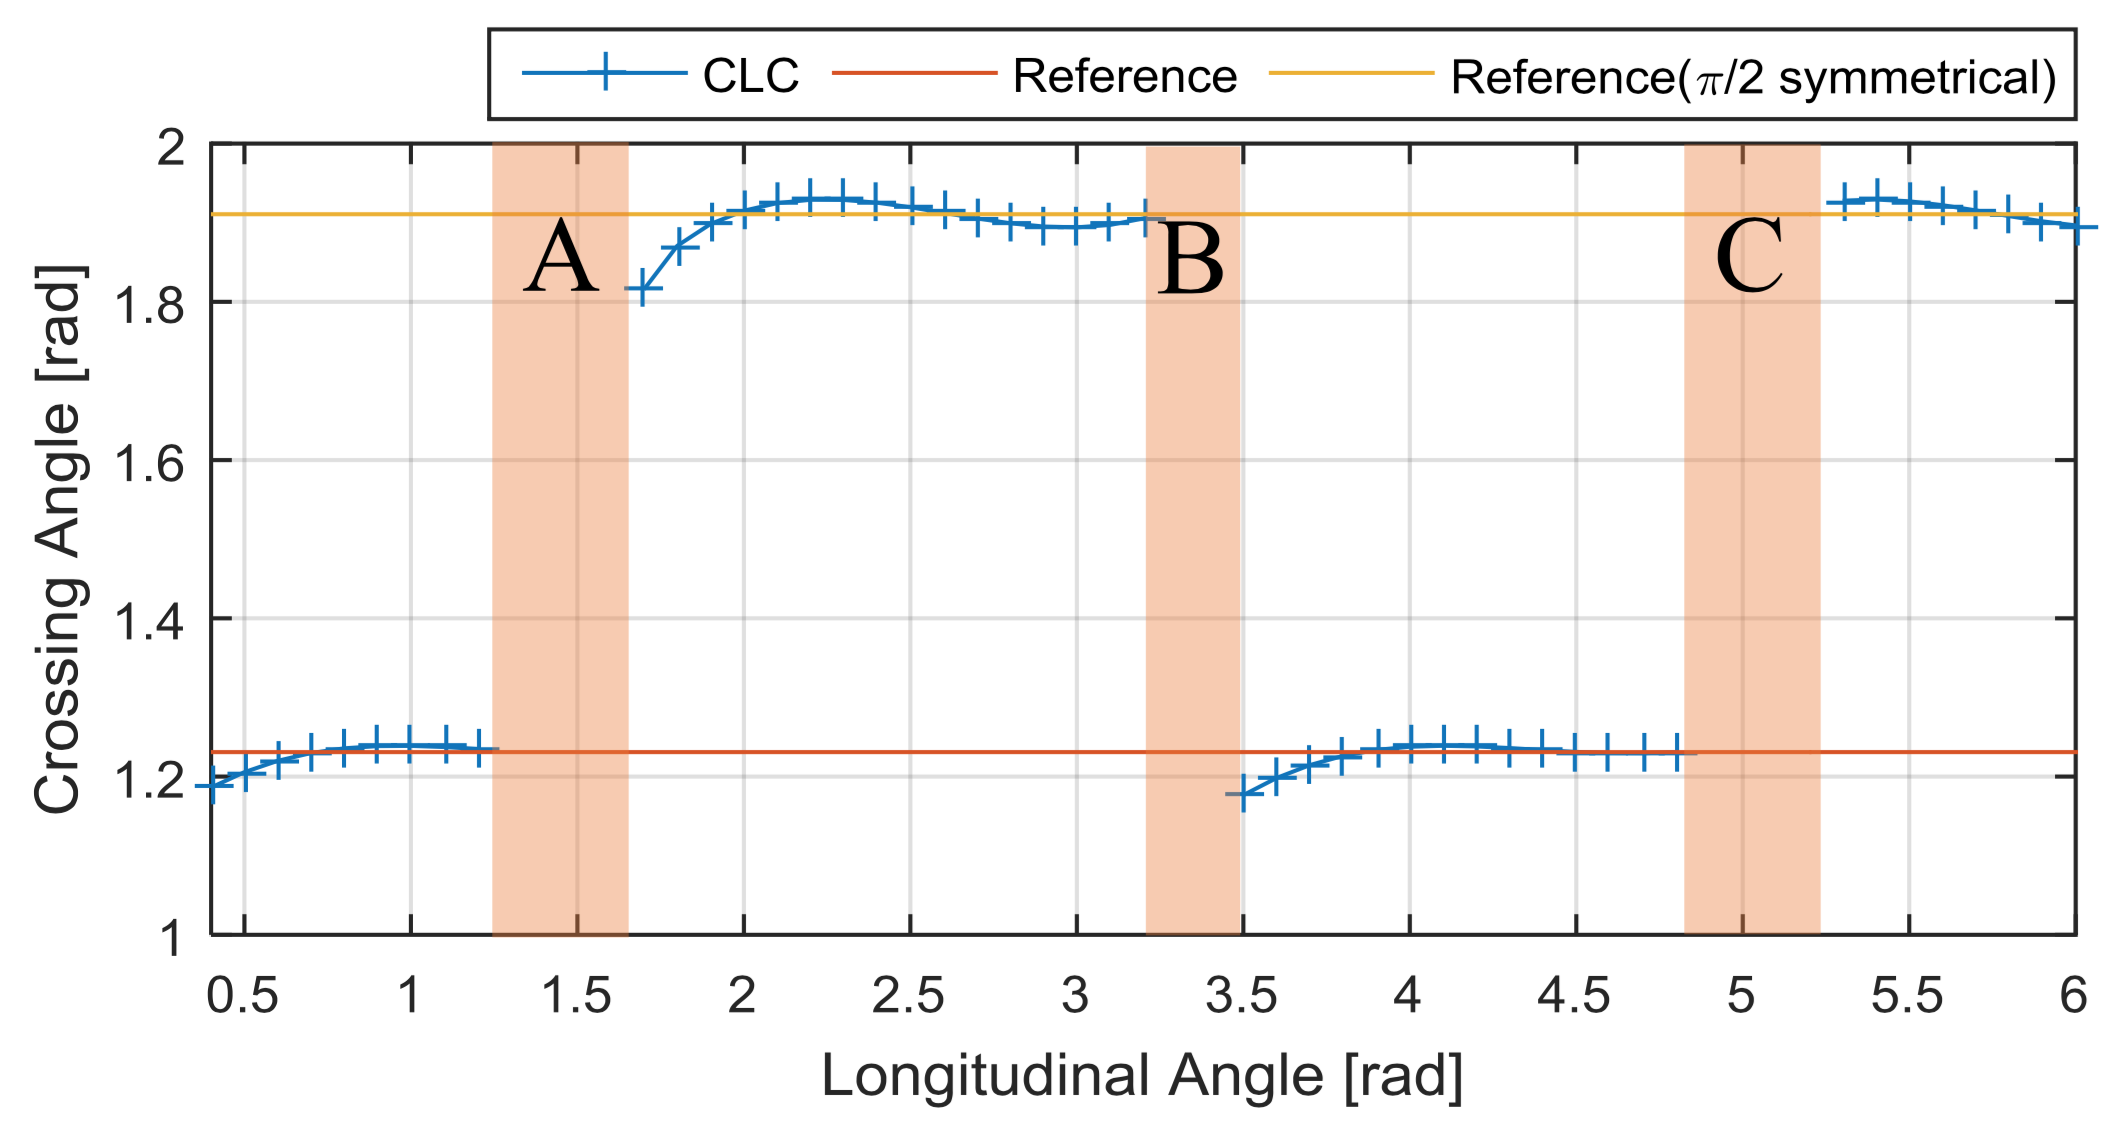
\includegraphics[width=360px]{img/ca_ang.png}
  \caption{The result of coupled line camera algorithm with respect to longitudinal angle }
\label{ca_ang}
\end{figure}
\newpage
\begin{figure}[!ht]
  \centering
	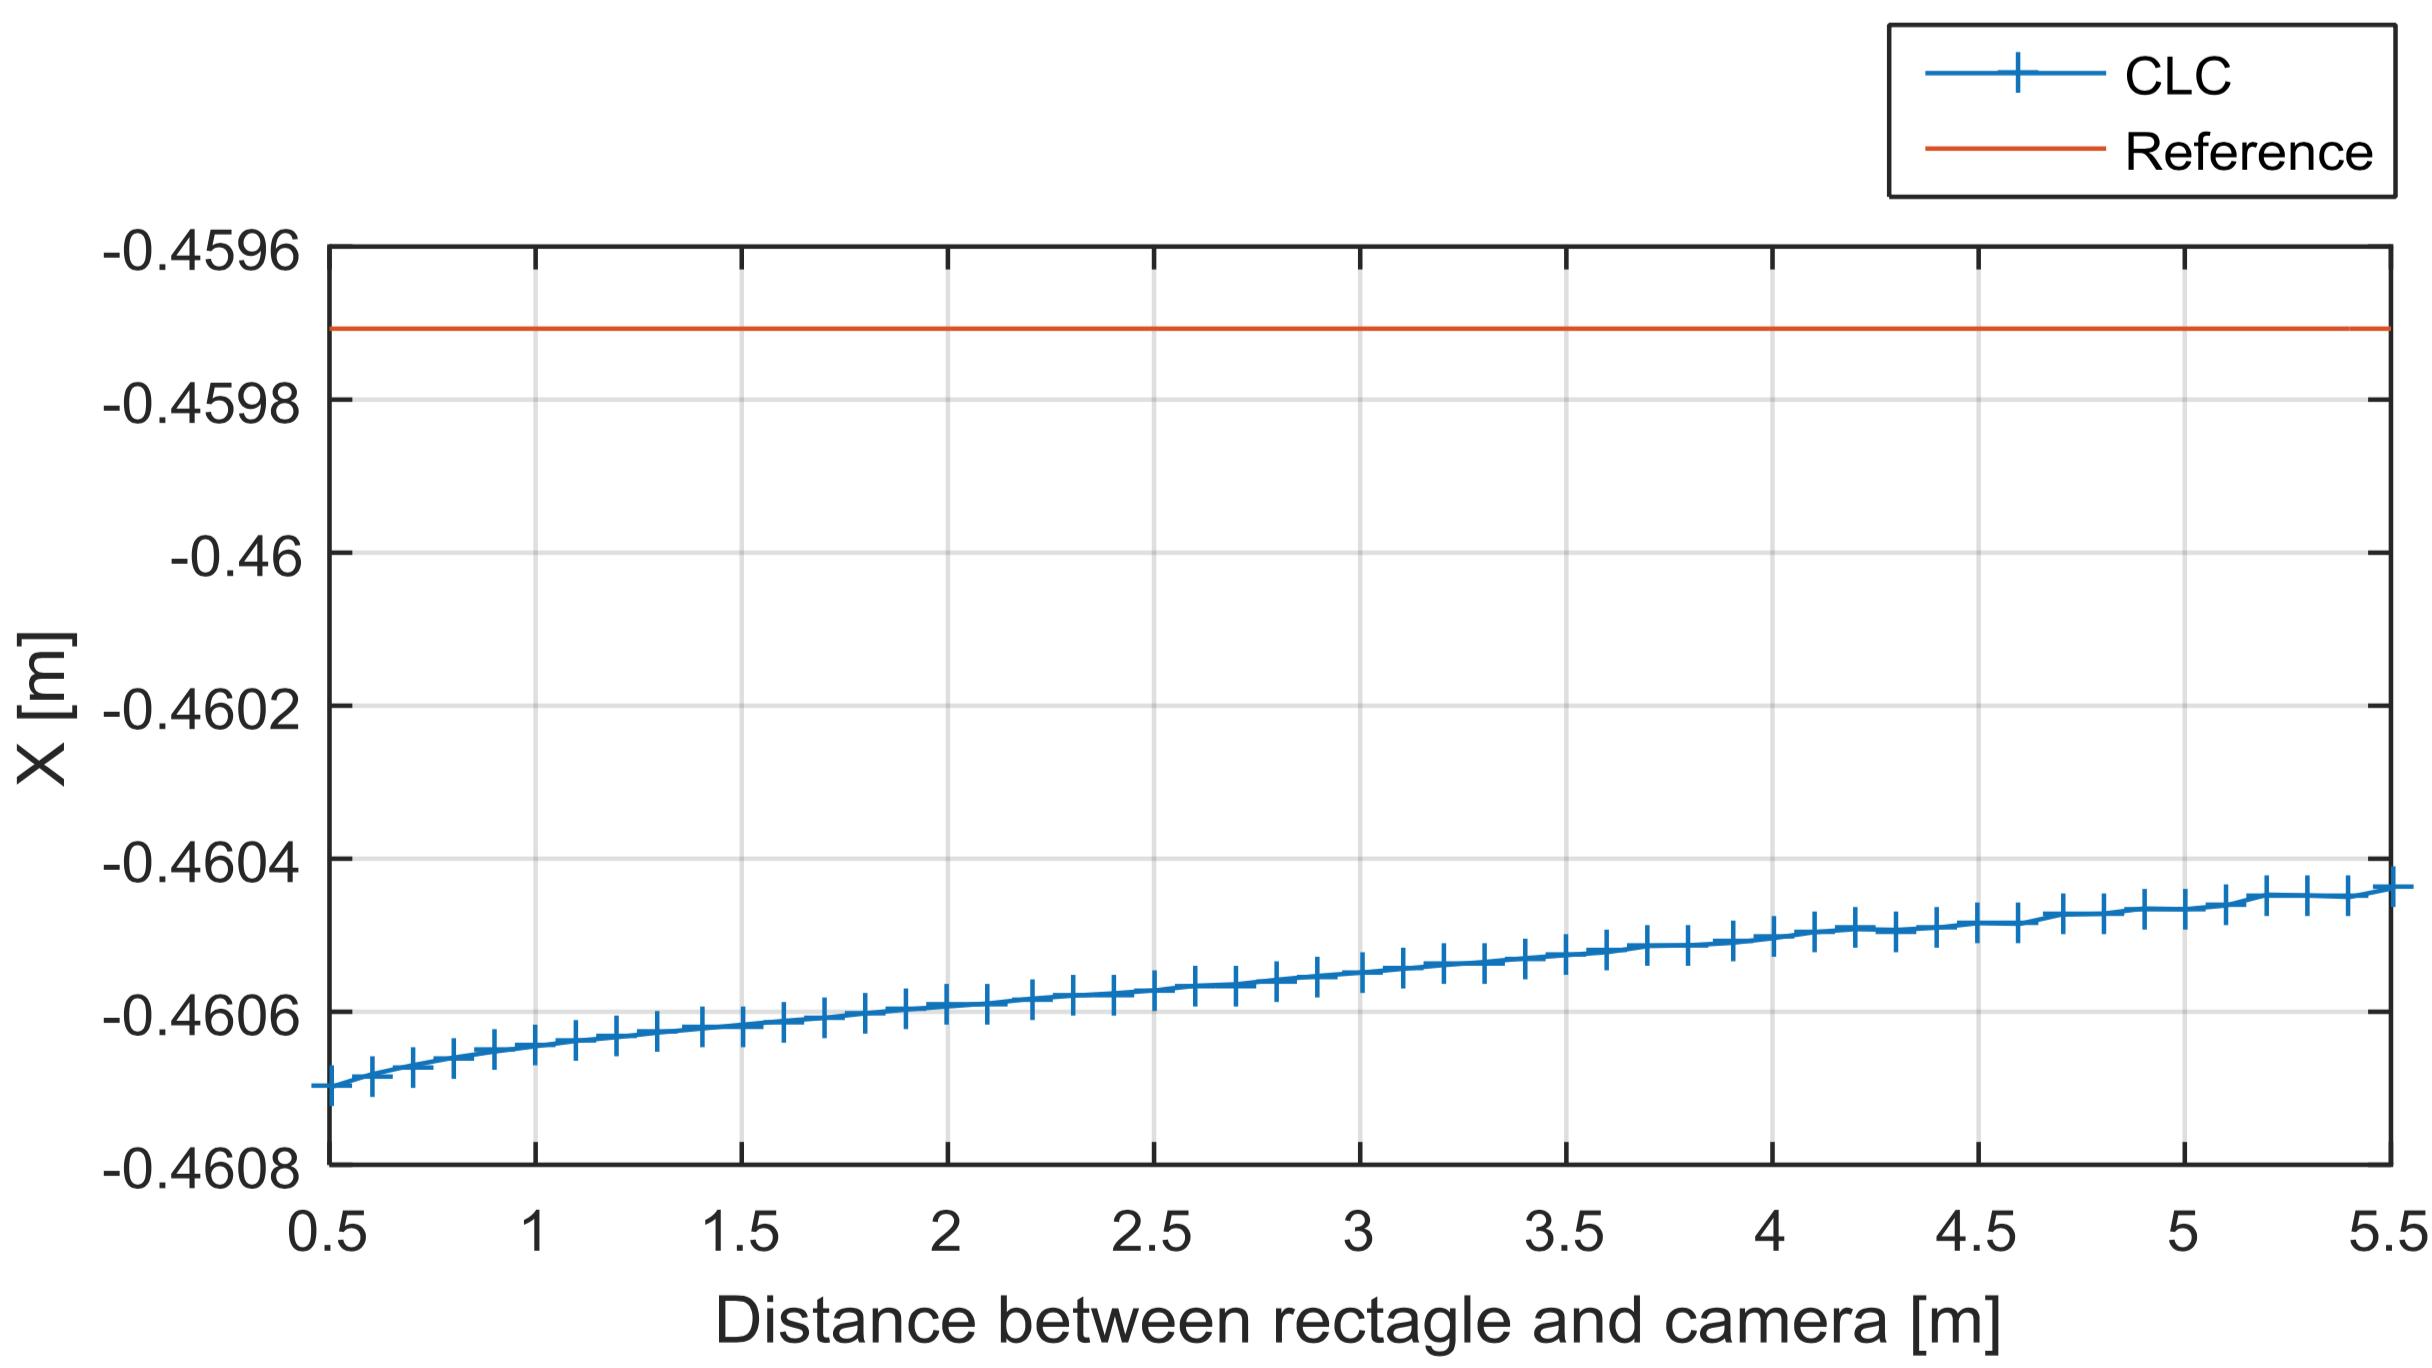
\includegraphics[width=360px]{img/X_d.png}
  \caption{The result of the proposed method and reference pose with respect to distance and X-axis }
\label{X_d}
\end{figure}
\begin{figure}[!ht]
  \centering
	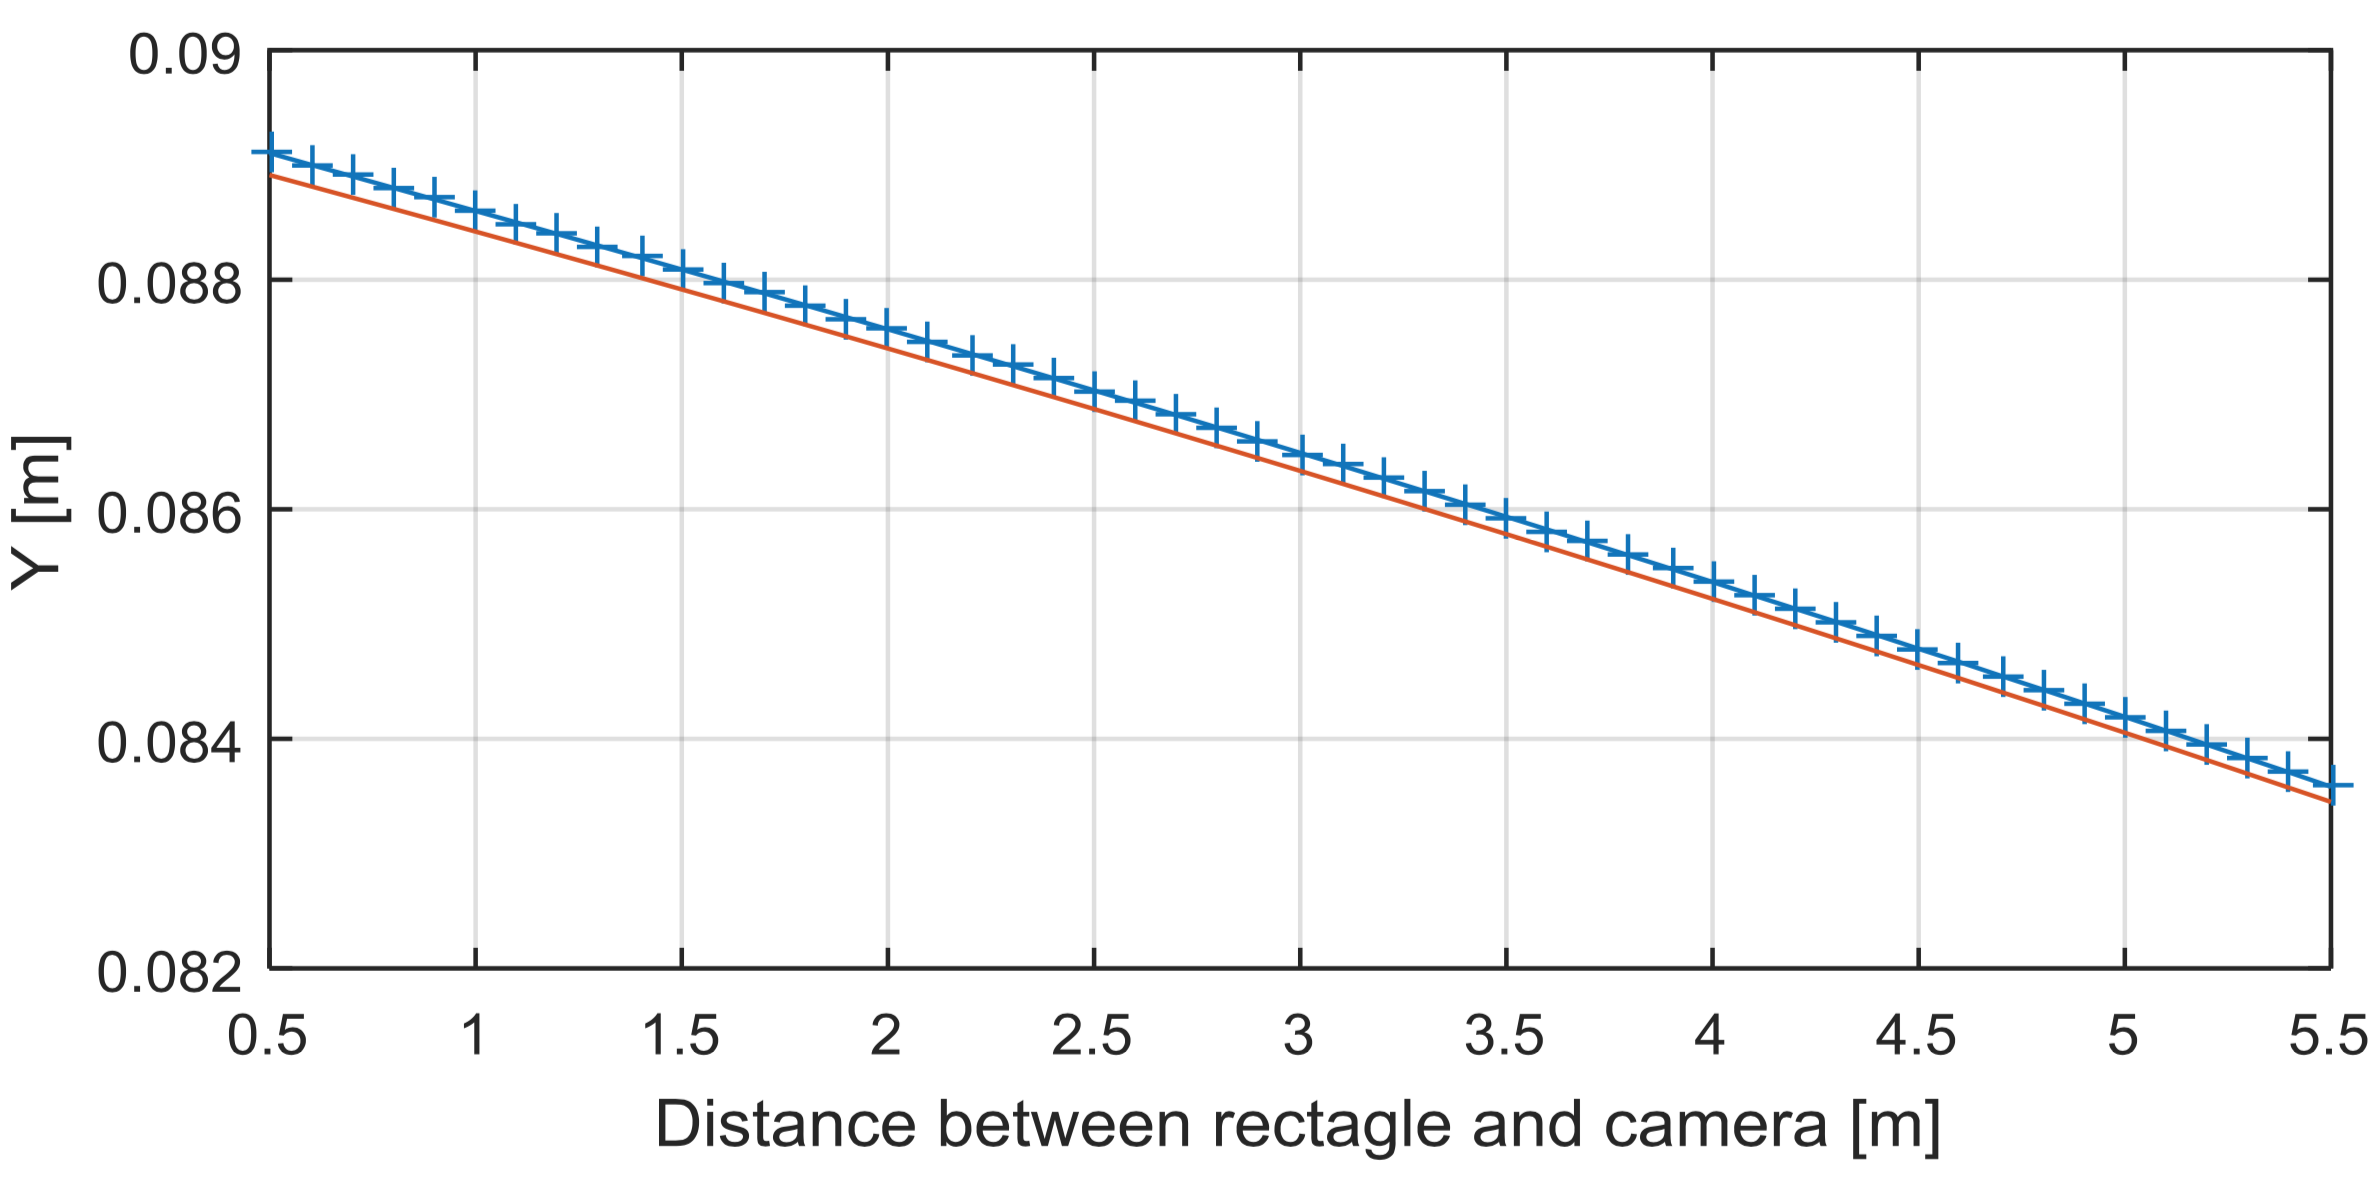
\includegraphics[width=360px]{img/Y_d.png}
  \caption{The result of the proposed method and reference pose with respect to distance and Y-axis }
\label{Y_d}
\end{figure}
\begin{figure}[!ht]
  \centering
	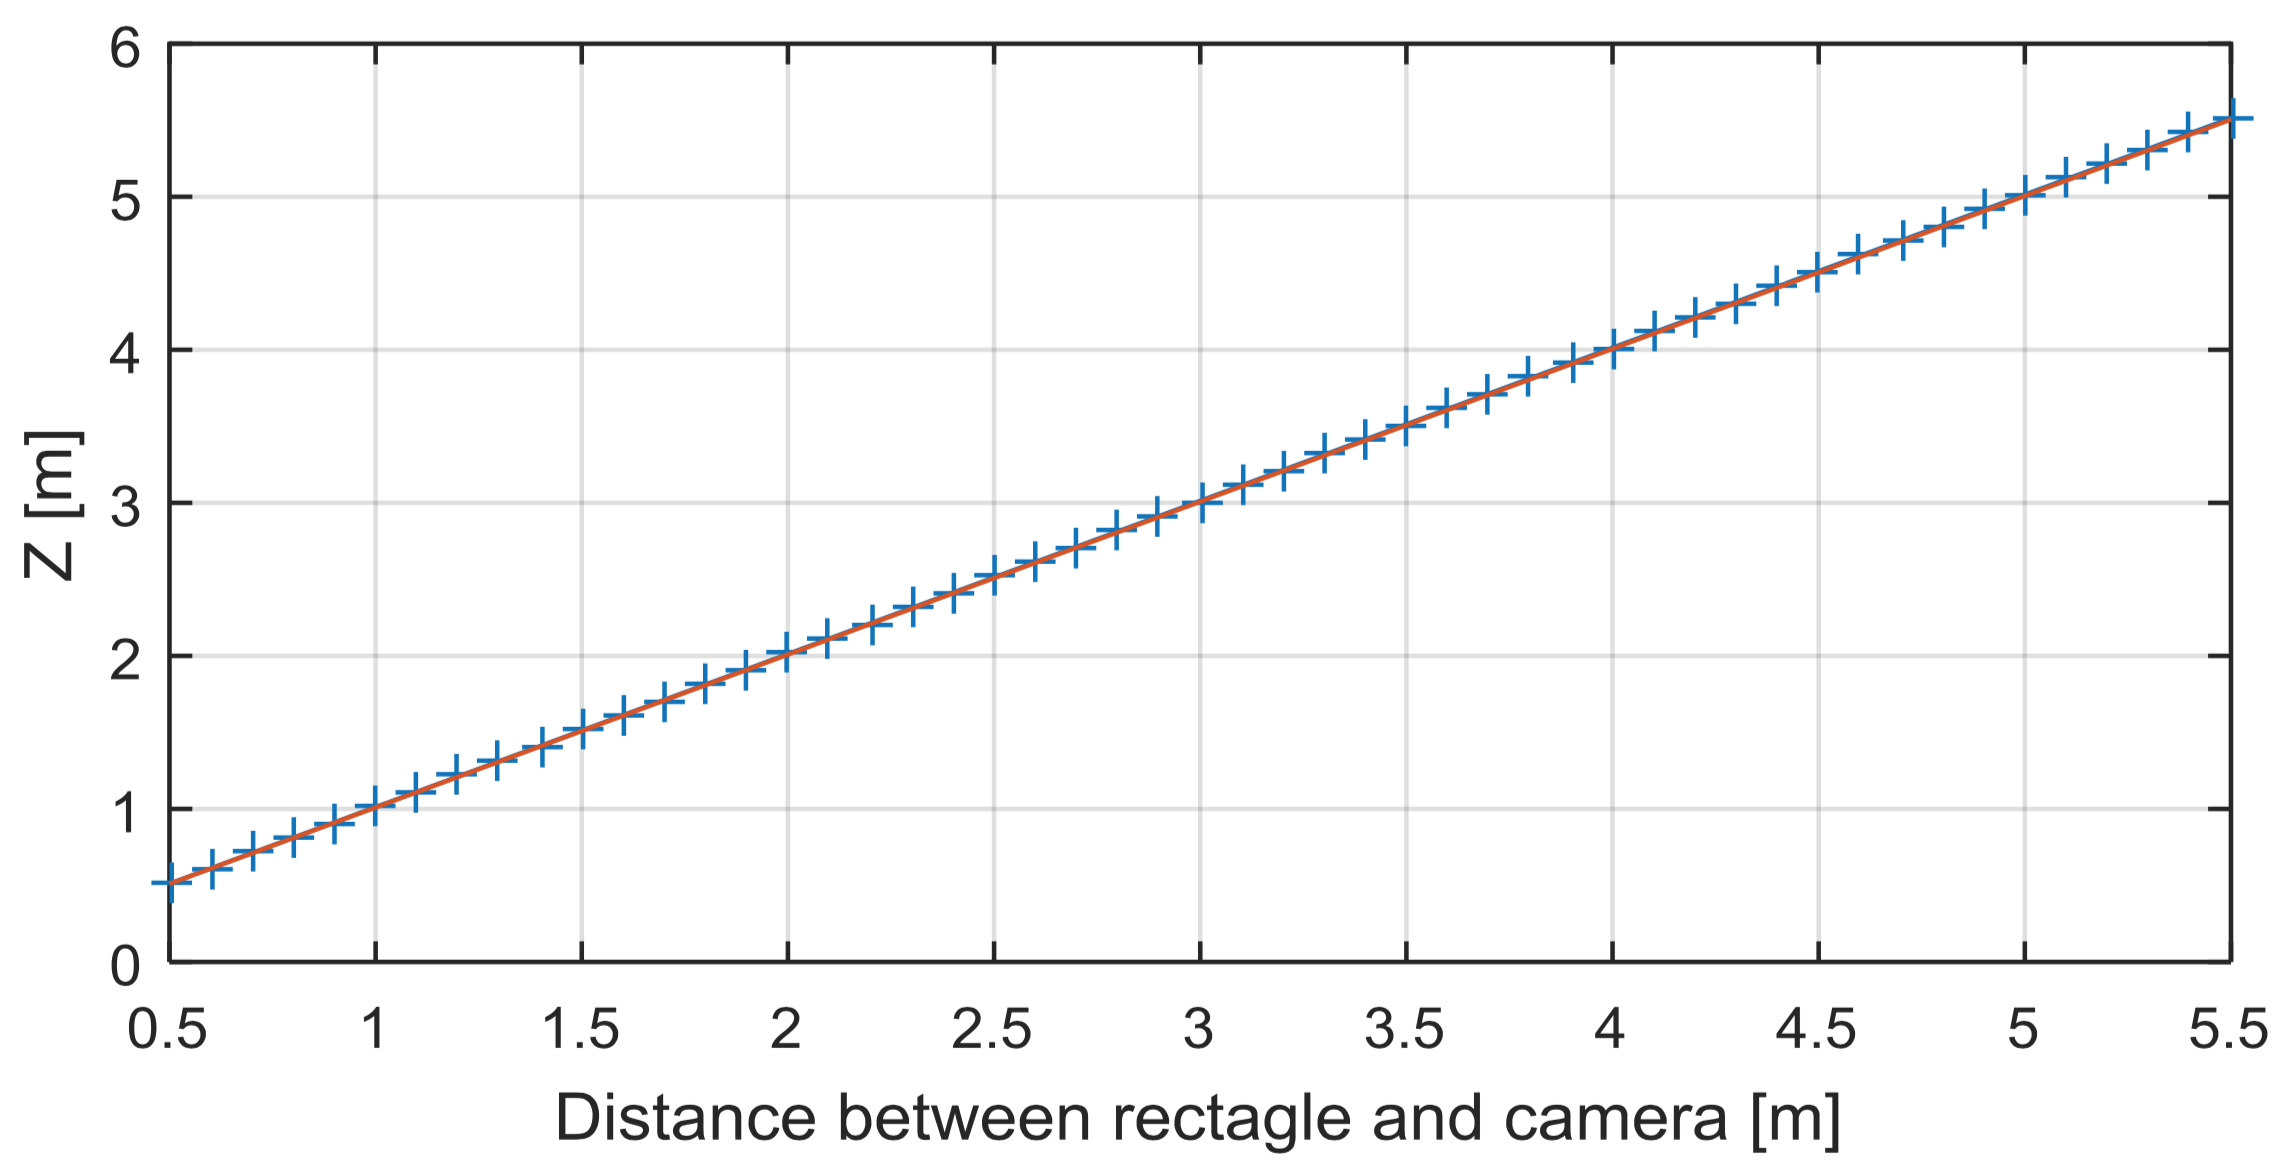
\includegraphics[width=360px]{img/Z_d.png}
  \caption{The result of the proposed method and reference pose with respect to distance and Z-axis }
\label{Z_d}
\end{figure}
\begin{figure}[!ht]
  \centering
	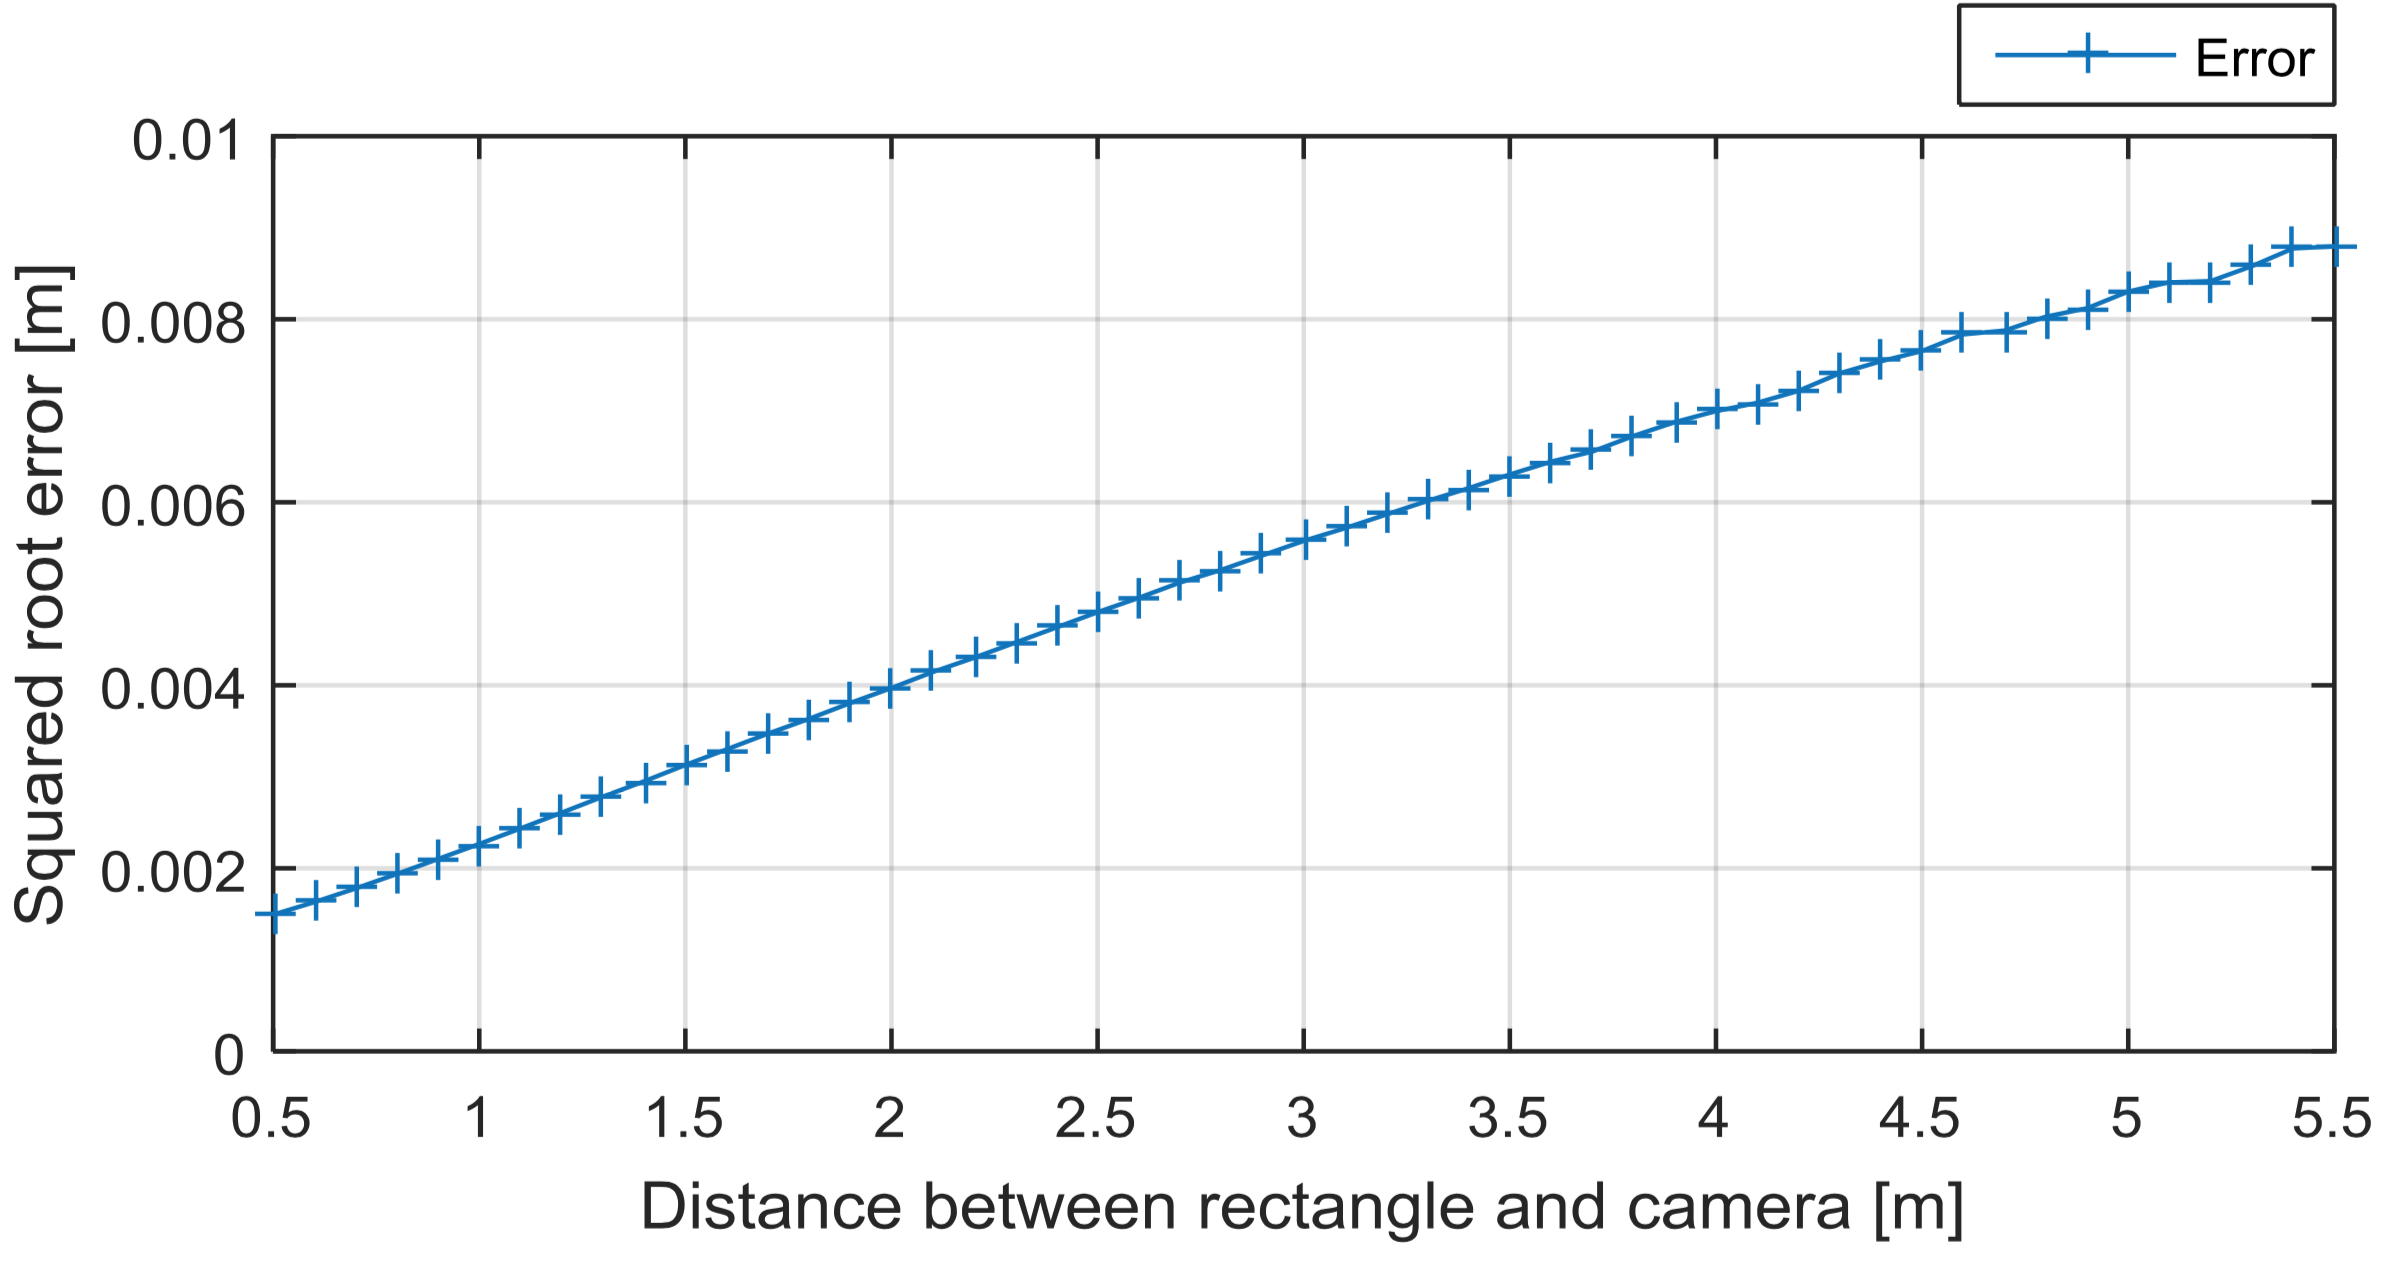
\includegraphics[width=360px]{img/RMS_d.png}
  \caption{The square root error of the proposed pose estimation method with respect to distance}
\label{RMS_d}
\end{figure}
\begin{figure}[!ht]
  \centering
	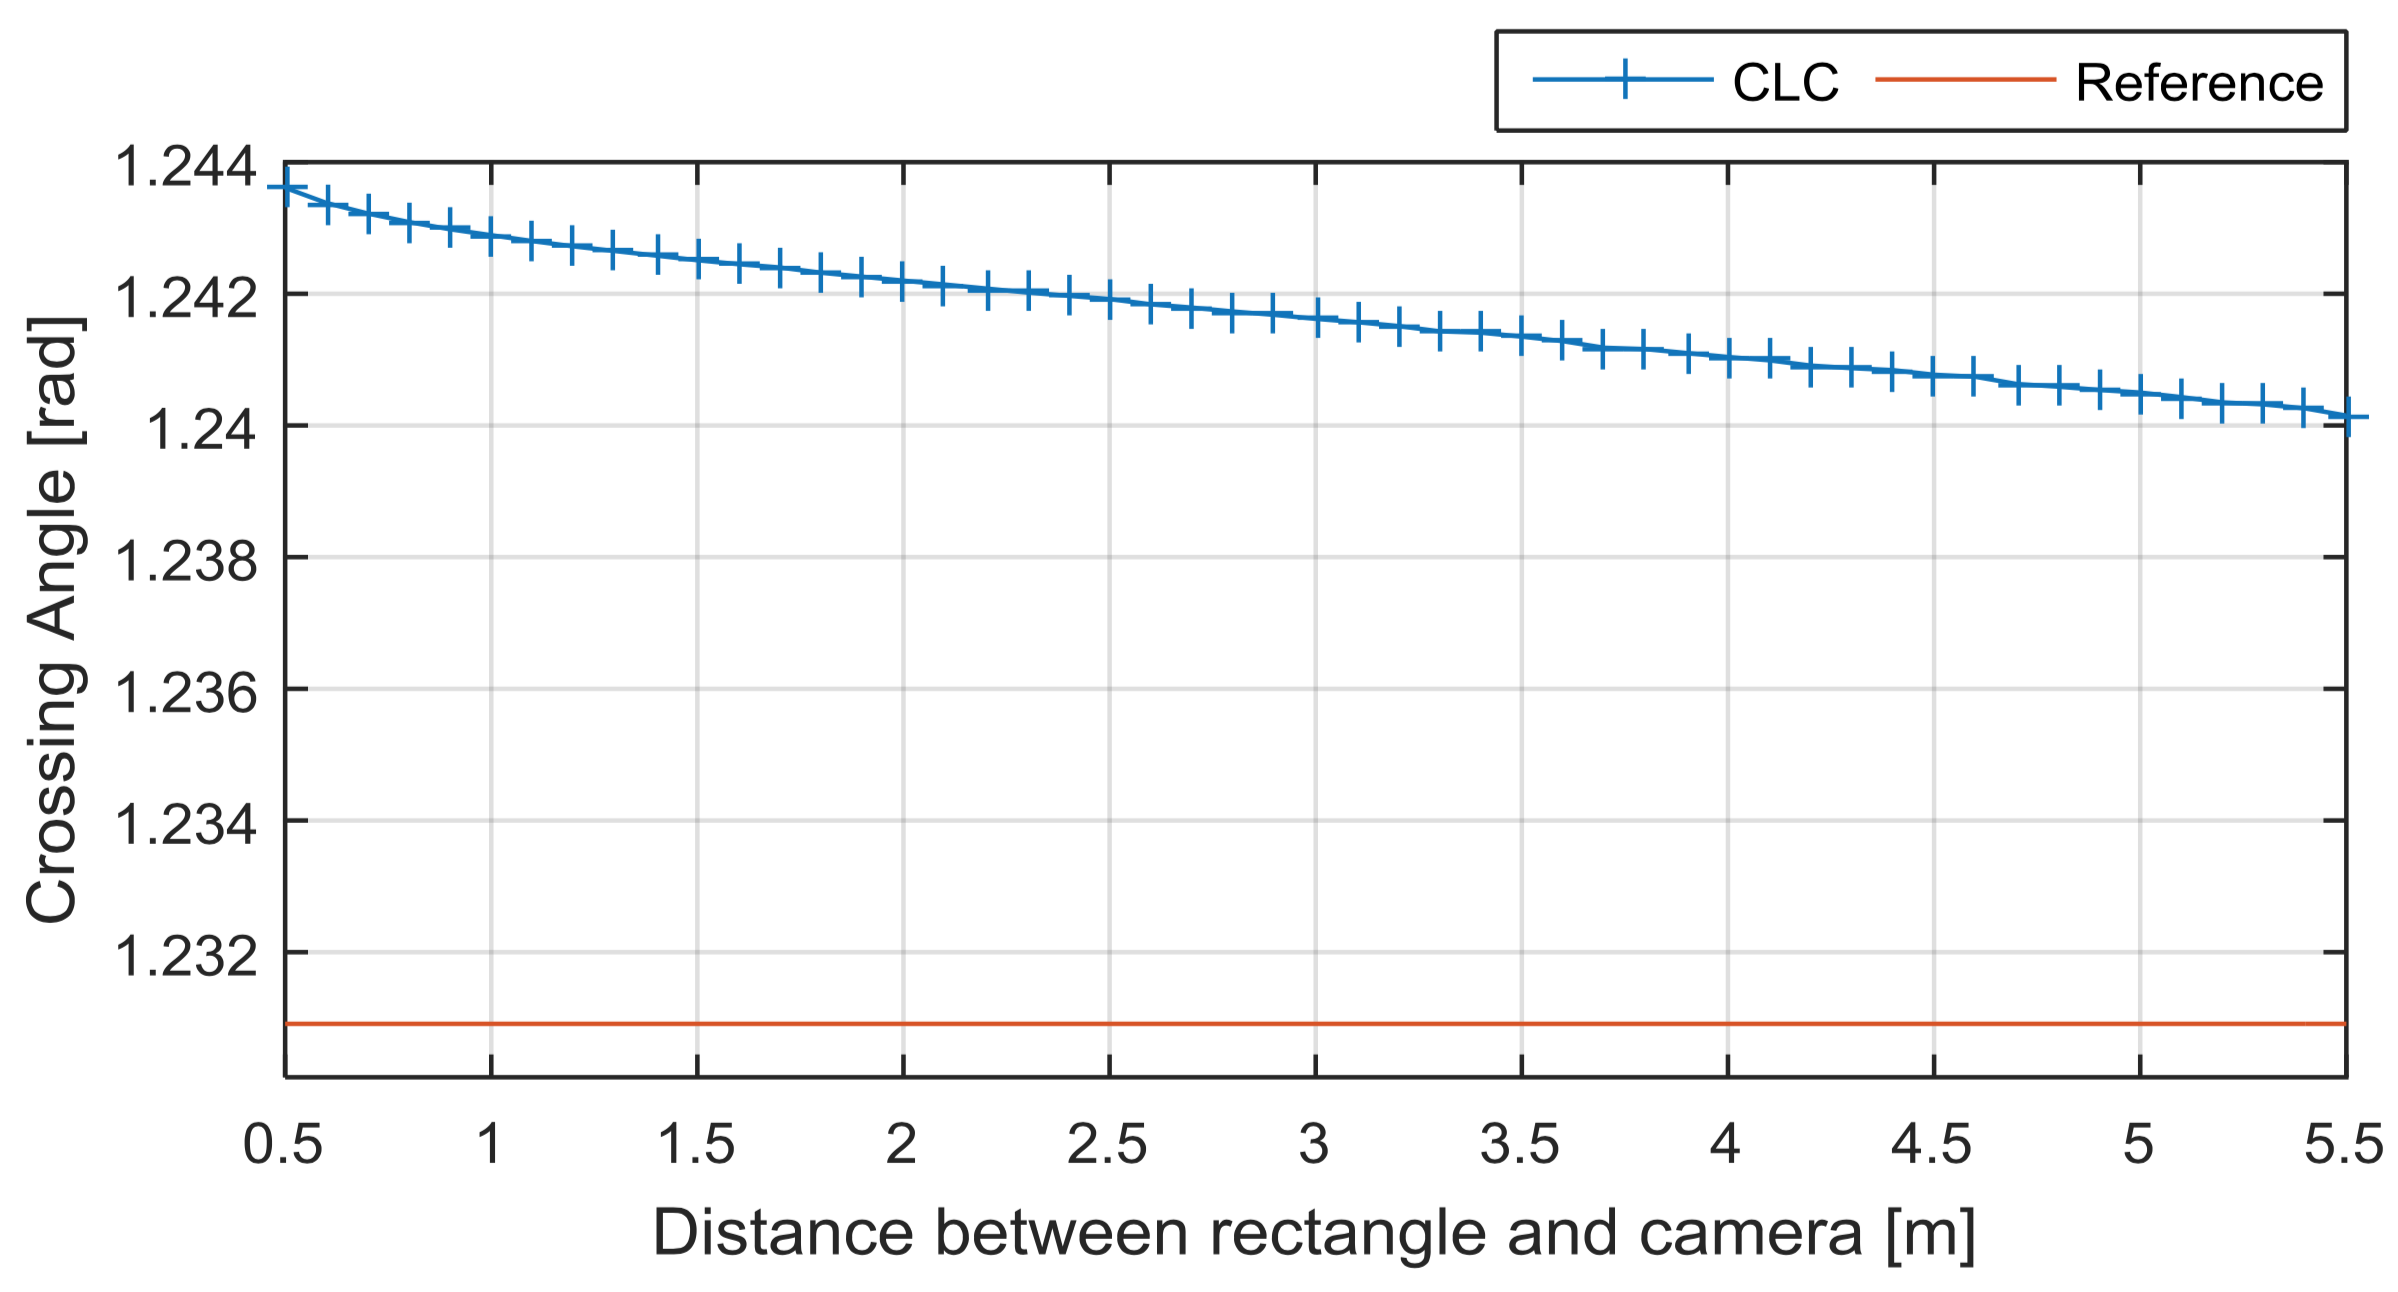
\includegraphics[width=360px]{img/ca_d.png}
  \caption{The result of coupled line camera algorithm with respect to distance }
\label{ca_d}
\end{figure}

\clearpage

\section{사각형 특징 기반 factor graph SLAM 성능 실험}
\subsection{KITTI Dataset 실험}
사각형 특징을 factor graph 기반의 SLAM으로 활용이 가능할 수 있는지 파악하기 위해 공개된 데이터를 이용하여 검증하였다. 데이터는 KITTI Benchmark Suite의 visual odometry 성능검증용 영상과 ground truth데이터 중 sequence07로 공개된 데이터를 사용하였다. 여기서 추출되는 주요 사각형 특징은  거울의 프레임, 창문, 간판과 같은 것으로, figure \ref{feature_kitti_01}, \ref{feature_kitti_02}, \ref{feature_kitti_03}에 소개되어 있다. KITTI Benchmark Suite에서 제공하는 영상은 0.54m의 baseline을 가지는 스테레오 카메라에서 취득한 영상으로 GPS/INS정보가 같이 동기되어 visual odometry 또는 visual SLAM에서 추정한 카메라의 이동경로를 ground truth와 비교하기 용이하다. 실험은 전체 영상이 아닌 시작 후 3미터 가량 회전하는 구간에 한해 수행하였다. Figure \ref{seq_07}에는 xz평면 상에서 실제 차량의 이동 궤적과 제안하는 방법이 추정한 궤적을 비교 한 것이고 figure \ref{seq07tl}는 0.5m 마다 이동 거리에 따른 위치 에러의 백분위를 표현한 그래프로 10\% 이내의 오차를 보여주었다. 
%지도를 작성하는 특징의 수는  --개이고 각 영상에서 평균 --개의 특징이 검출되어 위치 인식 및 지도 작성에 사용되었다
\clearpage

\begin{figure}[!ht]
  \centering
	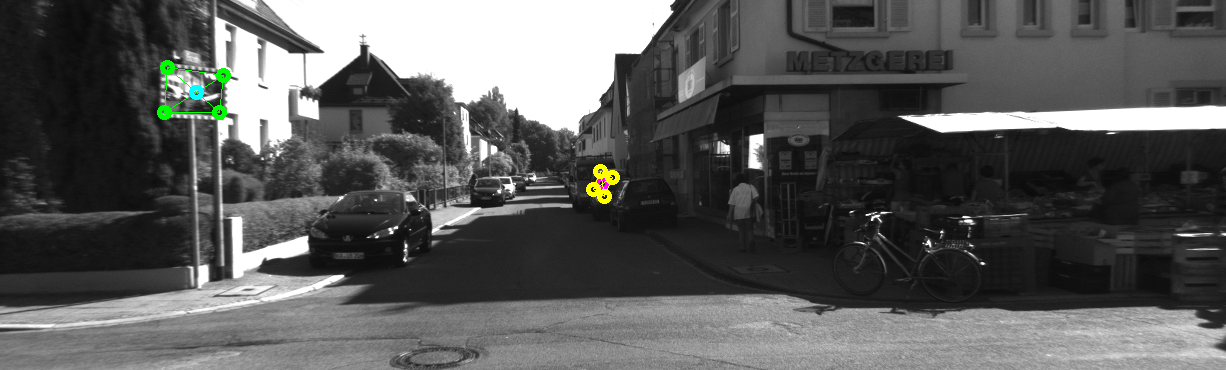
\includegraphics[width=380px]{img/feature_kitti_01.png}
  \caption{An example of rectangle feature in outdoor scene : The frame of mirror }
\label{feature_kitti_01}
\end{figure}

\begin{figure}[!ht]
  \centering
	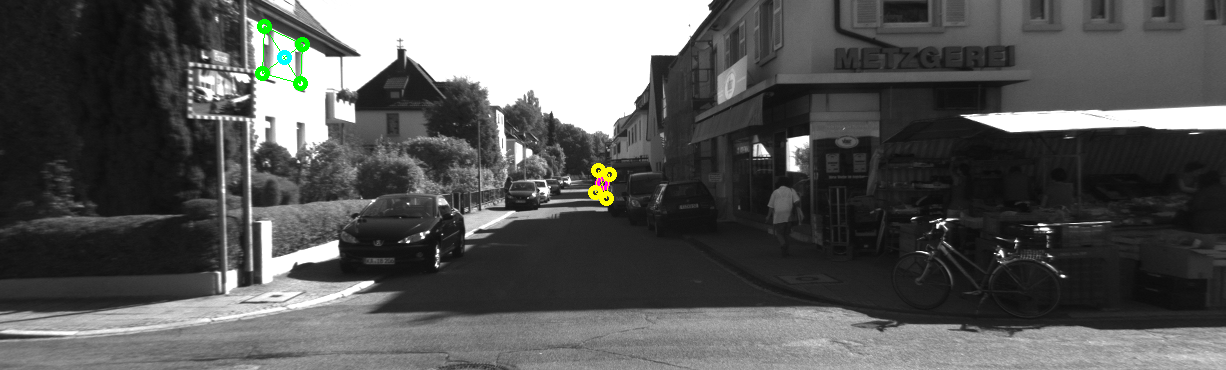
\includegraphics[width=380px]{img/feature_kitti_02.png}
  \caption{An example of rectangle feature in outdoor scene : Windows }
\label{feature_kitti_02}
\end{figure}

\begin{figure}[!ht]
  \centering
	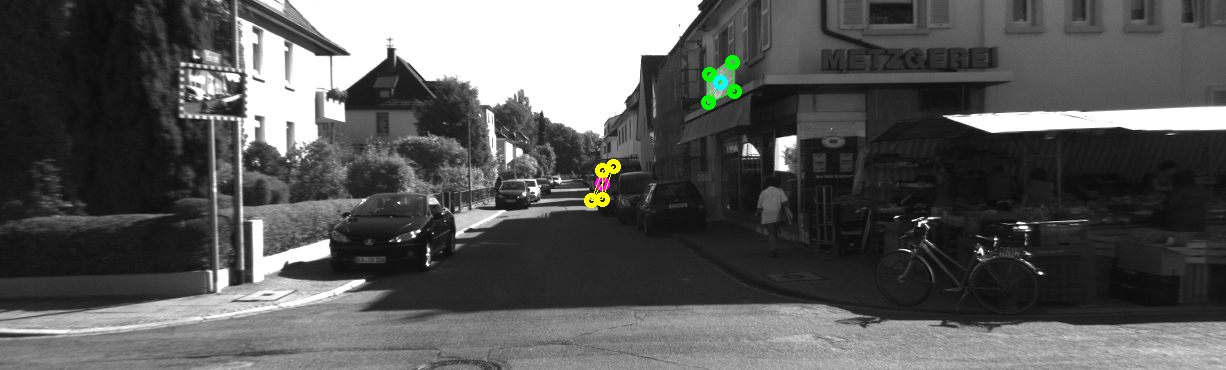
\includegraphics[width=380px]{img/feature_kitti_03.png}
  \caption{An example of rectangle feature in outdoor scene : Sign }
\label{feature_kitti_03}
\end{figure}

\clearpage
\begin{figure}[!ht]
  \centering
	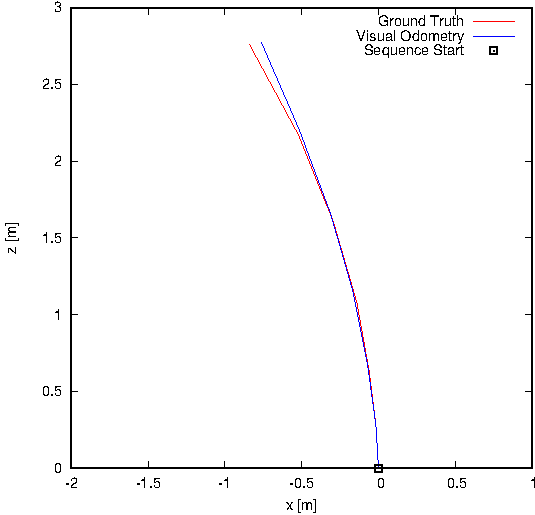
\includegraphics[width=380px]{img/seq_07.pdf}
  \caption{The result of proposed factor graph slam in sequence 07 of KITTI dataset}
\label{seq_07}
\end{figure}

\begin{figure}[!ht]
 \centering
	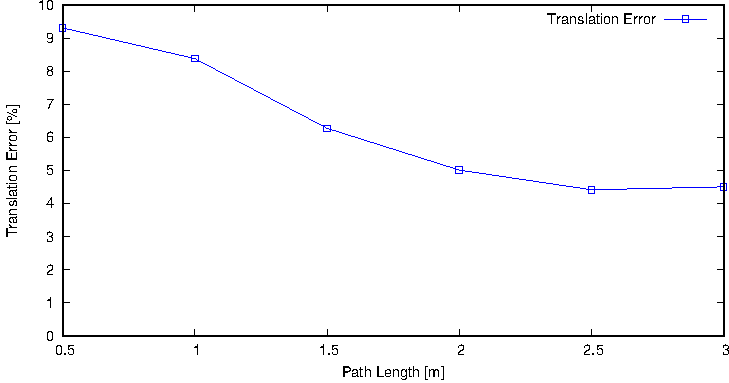
\includegraphics[width=360px]{img/seq07tl.pdf}
  \caption{The proportional translation error between proposed factor graph slam and ground truth in sequence 07 of KITTI dataset}
\label{seq07tl}
\end{figure}

%GPS, ORB-SLAM, libviso2, MFG
%\section{사각형 특징 기술자 매칭 성능 실험}
%\subsection{면 기반 매칭 방법과의 비교}
%\subsection{키포인트 추출 기반 매칭 방법과의 비교}

%%%%%%%%%%%%%%%%%%%%%%%%%%%%%%%%%%%%%%%%%%%%%%%%%%%%%%%%%%%%%%%%%%%%%%%%%%%%%%%%%%%%%%%%%%%%%%%%%%%%%%%%%%%%%%%%%%%
%%%%%%%%%%%%%%%%%%%%%%%%%%%%%%%%%%%%%%%%%%%%%%%%%%%%%%%%%%%%%%%%%%%%%%%%%%%%%%%%%%%%%%%%%%%%%%%%%%%%%%%%%%%%%%%%%%%
%%%%%%%%%%%%%%%%%%%%%%%%%%%%%%%%%%%%%%%%%%%%%%%%%%%%%%%%%%%%%%%%%%%%%%%%%%%%%%%%%%%%%%%%%%%%%%%%%%%%%%%%%%%%%%%%%%%
\chapter{결론 및 향후 연구}
본 논문에서는 사각형 특징을 이용하여 위치와 자세를 복원하고 그를 factor graph형태로 구성하여 위치 인식과 특징 지도를 작성하는 방법을 제안하였다. 임의의 영상 평면 상 사변형이 입력으로 주어졌을 때 선분카메라쌍 알고리즘을 이용하여 종횡비를 알 수 없는 실세계의 직사각형을 해석적으로 복원하고, 그를 이용하여 homography를 구성하여 미리 알려진 카메라의 내부 파라미터 성분을 이용하여 정규화 한 뒤 카메라와 사각형 특징간의 상대 위치와 자세를 복원하였다. 이 때 사각형의 실제 크기를 알 수 없어 생기는 모호성을 해결하기 위해 카메라의 스테레오 구성을 가정한다. 스테레오 카메라가 x축에 대해 정렬되어있고 baseline값이 고정되어 있을 때 사각형과 카메라 사이의 정확한 위치와 자세를 추정하는 방법에 대해 제안하고 실험을 통해 특징 추출이 잘 이루어졌을 때 제안하는 위치 및 자세 추정의 성능이 준수함을 보였다. 추출된 특징과 상대 위치는 factor graph형태로 구성하고 negative log likelyhood 추정으로 접근하여 비선형 최소자승 문제를 정의한 뒤, 선형화를 통해 선형 최소자승 문제로 치환하여 cholesky factorization을 통해 해를 구한다. 이 때 사용할 수 있는 사각형 특징 추출 방법으로 선분 추출 기반의 방법과 영상 분할 기반의 방법을 제안하고 영상 분할 기반의 접근이 보다 유효함을 주장하였다. 제안한 전체 시스템은 카메라 기반의 위치 추정 시스템의 성능 분석용으로 널리 사용되는 KITTI Benchmark Suite위에서 실험이 수행되었다.\\
이 연구에서 사용한 특징 추출 방법은 영상 분할 방법을 기반으로 하여 조명의 변화에 따른 음영의 변화에 민감하여 복수의 유사한 사각형이나 실제 사각형이 아닌 그림자에 의한 형상을 추출하는 등의 문제가 발생할 수 있다. 향후 연구에서는 직사각형이 투영변환에 의해 왜곡되어 사변형으로 나타날 때 두 개 이하의 소실점과 반드시 연관이 있음을 이용하여, 소실점 추출과 선분 추출 방법을 융합하여 특징 검출 성능을 높이고자 한다. 또한 사각형 특징의 우수한 내부 정보를 효과적으로 부호화하는 특징 기술자에 관한 연구와 대규모의 구동 환경에서 loop closure성능을 실험하여 사각형 기반 SLAM의 독립적인 성능과 기존 SLAM방법과의 융합 결과의 분석도 염두에 두고 있다.
%%%%%%%%%%%%%%%%%%%%%%%%%%%%%%%%%%%%%%%%%%%%%%%%%%%%%%%%%%%%%%%%%%%%%%%%%%%%%%%%%%%%%%%%%%%%%%%%%%%%%%%%%%%%%%%%%%%
% set second argument of \begin to the number of references
% (used to reserve space for the reference number labels box)

\bibliographystyle{IEEEtran}%...는 bst 파일의 이름(확장자 없이)
\bibliography{ThesisBibTeX.bib}%...는 bib 파일의 이름(확장자 없이)
%\begin{thebibliography}{1}
%\bibitem{greenberg}
%A. Greenberg, J. Hamilton, D.A. Maltz, and P. Patel,
%\emph{The cost of a Cloud: Research Problems in Data Center Networks},
%ACM SIGCOMM Computer Communication Review (CCR), 
%Vol. 39, No. 1, pp. 68-73, January 2009.
%
%\bibitem{wallin}
%S. Wallin, V. Leijon, 
%\emph{Telecom Network and Service Management: An Operator Survey}, 
%MMNS, 2009.
%
%\bibitem{hscalability}
%Wikipedia, \emph{Horizontal Scalability},
%\url{http://en.wikipedia.org/wiki/Scalability#Scale_horizontally_.28scale_out.29}
%
%\end{thebibliography}


\chapter*{감사의 글}

먼저 지능로봇연구실의 지도교수님이시며 연구에 대한 많은 동기를 부여해 주시고 학부, 석사기간 내내 다방면에서 도움을 주신 김곤우교수님께 감사드립니다. 학부 과정에서 가장 유익하였던 컴퓨터 구조 강의를 해 주시고, 본 논문의 지도교수를 대신 맡아 신경 써 주신 박찬식교수님, 제어에 대한 궁금증이 있을 때 찾아가면 흔쾌히 알려주시며 인생에 대해서도 조언을 주신 김영철교수님과 훌륭한 강의로 식견을 넓혀 주신 권오욱교수님, 김진훈교수님, 박태형교수님께 감사의 말씀 드립니다. 12회 현대 자율차 대회 준비로 같이 고생했던 CBNU-Clothoid팀 종언이형, 귀우형, 태수형, 준기형, 지문이형, 주영이형, 신수연씨, 산자부 공용차량 경진대회를 준비했던 우진이형, 상환씨, 범기씨, 전임팀장으로 제어시스템설계와 팀 운영 관련 많은 조언을 해주신 민경득박사님, 현재 13회 대회를 준비하며 고생하고있는 민이형, 준형씨, 지덕씨께 모두 감사의 말씀 드립니다.\\
2012년부터 학부 연구생으로 충북대학교 지능로봇연구실에 들어와 약 5년간 교수님과 함께 연구실을 키워가며 같이 생활한 모든 랩 구성원에게 정말 감사하게 생각합니다. 학부/석사 과정 중 경제적으로 굉장히 어려웠을 때 많은 힘이 되어 주고 3년간 거의 모든 연구실의 행정 처리를 도맡아 하시며 고생하신 창섭이형이 없었으면 석사과정 졸업이 불가능했을지도 모르겠습니다. 지금 2학년 과정에 계신 도형이형, 동규형, 은성이형, 성진이형, 1학년 과정에 계신 중선이형, 현수형께는 나이 어린 놈이  예의 없게 하는 말을 묵묵히 들어주셔 감사하면서 죄송하다는 말씀을 드립니다. 모두들 처음 연구실 들어올 때의 모습과 각자 위치에서 고생하던 모습이 아직 선합니다. 밤까지 동국대로 출장 다니며 고생하신 도형이형, 광역 과제로 천안으로 출퇴근하다시피 다니시던 동규형과 성진이형이 특히 수고하셨습니다. 이듬해 산자부 자율차 대회에 참가해서 제 괴롭힘(?)을 받으며 굉장히 스트레스가 많았을 것인데 최종 결과로 보답해드리지 못해 죄송할 따름입니다. 개인적으로는 마지막 대구의 한 모텔에서 4일간 에너지 드링크를 세워두고 코딩했던 철야 경험은 연구실 생활 중에서 손에 꼽는 추억이 되었습니다. 형들께도 힘들었지만 의미있던 경험이 되어 있으면 저도 보람찰 것 같습니다. 남은 석사 기간동안은 좋은 연구 주제로 훌륭한 결과 얻으실 수 있기를 바라겠습니다. 그리고 5년간 함께 공부하고 고생한 영보에게는 정말 감사합니다. 대학 생활의 80\%이상을 이 친구와 함께 했지만 서로 의지가 되지는 못할 망정 항상 따라가기 벅찬 기분이었습니다. 근면성실한 품성과 출중한 기본기를 바탕으로 훌륭하게 연구를 수행하고 제가 미처 놓치거나 무시한 부분을 들춰주고 지적해 주어 많은 공부가 되었습니다. 학부과정때 광역과제와 충주APC과제, 해양연과제 등 많은 일을 함께 처리했지만 정작 연구에 대해서는 서로 관련된 주제로 심도있게 토의하고 협력한 결과를 내지 못하여 아쉽게 생각합니다. 서로 다른 곳에서 열심히 공부해서 추후 좋은 연구 주제로 다시 같이 머리를 맞댈 수 있는 날이 오기를 기대합니다.\\
\begin{flushright}
\vspace{1cm}
이재민 배상
\end{flushright}

\end{document}



